\documentclass[12pt,a4paper]{article}

\usepackage{xurl}
\usepackage{amsmath}
\usepackage{tabularx} % Thư viện giúp bảng tự động co giãn
\usepackage[utf8]{inputenc}
\usepackage{float}
\usepackage[T5]{fontenc} % Hỗ trợ tiếng Việt chuẩn
\usepackage[vietnamese]{babel}
\usepackage{geometry}
\usepackage{graphicx}
\usepackage[table]{xcolor} % Hỗ trợ đổ màu bảng [table] rất quan trọng
\usepackage{tikz}
\usepackage{bytefield}    % Vẽ sơ đồ bit chuyên nghiệp (Phần 2 cần)
\usepackage{caption}      % Quản lý chú thích hình ảnh/bảng biểu
\usepackage[hidelinks]{hyperref}     % Tạo mục lục có thể nhấn vào được (link)
\usepackage{tikz}
\usetikzlibrary{positioning, arrows.meta, backgrounds, fit}
\usepackage{listings}
\usepackage{xcolor} % Để tô màu cho code
\usepackage{hyperref} % Gói lệnh để tạo liên kết
\hypersetup{
    colorlinks=true,
    linkcolor=blue,
    filecolor=magenta,      
    urlcolor=blue,        % Màu của liên kết GitHub sẽ là màu xanh
}
% Cấu hình cơ bản cho khối code Verilog
\lstset{
    basicstyle=\ttfamily\small,
    keywordstyle=\color{blue}\bfseries,
    commentstyle=\color{green!60!black},
    stringstyle=\color{red},
    numbers=left,
    numberstyle=\tiny\color{gray},
    stepnumber=1,
    frame=single,
    breaklines=true
}

\usetikzlibrary{calc}


\definecolor{BKB}{RGB}{0, 84, 166} 
\geometry{
    a4paper,
    left=30mm,
    right=20mm,
    top=20mm,
    bottom=20mm
}


\renewcommand{\arraystretch}{1.2} 
\linespread{1.2} 


\begin{document}

    
    \begin{titlepage}
    \begin{tikzpicture}[remember picture, overlay]
        % Khung viền
        \coordinate (NW) at ($(current page.north west) + (2.5cm,-1.5cm)$);
        \coordinate (SE) at ($(current page.south east) + (-1.5cm,1.5cm)$);
        
        \draw[BKB, line width=2.5pt] (NW) rectangle (SE);
        \draw[BKB, line width=0.8pt] ($(NW) + (0.15,-0.15)$) rectangle ($(SE) + (-0.15,0.15)$);
        
        \def\side{0.6cm}
        \draw[BKB, line width=2pt] ($(NW) + (0,-\side)$) -- (NW) -- ($(NW) + (\side,0)$);
        \draw[BKB, line width=2pt] ($(NW |- SE) + (0,\side)$) -- (NW |- SE) -- ($(NW |- SE) + (\side,0)$);
        \draw[BKB, line width=2pt] ($(SE |- NW) + (-\side,0)$) -- (SE |- NW) -- ($(SE |- NW) + (0,-\side)$);
        \draw[BKB, line width=2pt] ($(SE) + (0,\side)$) -- (SE) -- ($(SE) + (-\side,0)$);
    \end{tikzpicture}
    
    \begin{center}
        {\fontsize{14}{16}\selectfont \textbf{ĐẠI HỌC QUỐC GIA TP. HỒ CHÍ MINH} \par}
        {\fontsize{14}{16}\selectfont \textbf{TRƯỜNG ĐẠI HỌC BÁCH KHOA} \par}
        {\fontsize{14}{16}\selectfont \textbf{KHOA KHOA HỌC VÀ KỸ THUẬT MÁY TÍNH} \par}
        
        \vspace{0.8cm}
        
        \ifcsname includegraphics\endcsname
            
\includegraphics[height=3.2cm]{logo} 
        \fi
        
        \vspace{0.8cm}
        
        % Phần Môn học, Mã môn, Học kỳ
        {\fontsize{13}{15}\selectfont \textbf{MÔN HỌC: THIẾT KẾ LUẬN LÝ VỚI HDL} \par}
        {\fontsize{13}{15}\selectfont \textbf{MÃ MÔN HỌC: CO1025} \par}
        {\fontsize{13}{15}\selectfont \textbf{HỌC KỲ: 252} \par}
        
        \vspace{0.8cm}
        {\fontsize{16}{18}\selectfont BÁO CÁO ĐỒ ÁN MÔN HỌC \par}
        
        \vspace{0.4cm}
        \begin{tikzpicture}
            \draw[BKB, line width=1.5pt] (0,0) -- (12,0);
        \end{tikzpicture}
        \vspace{0.4cm}
        
        {\fontsize{22}{26}\selectfont \textbf{THIẾT KẾ RISC CPU ĐƠN GIẢN} \par}
        
        \vspace{0.4cm}
        \begin{tikzpicture}
            \draw[BKB, line width=1.5pt] (0,0) -- (12,0);
        \end{tikzpicture}
    \end{center}
    
    \vspace{1cm}
    
    
    \begin{center}
        \renewcommand{\arraystretch}{1.5}
        \begin{tabular}{l l}
            \textbf{Giảng viên hướng dẫn:} & HUỲNH PHÚC NGHỊ \\
            \textbf{Lớp:}                  & L01 \\
            \textbf{Nhóm thực hiện:}       & 9 \\
        \end{tabular}
    \end{center}
    
    \vfill
    
    % Danh sách thành viên
    \begin{center}
        \textbf{DANH SÁCH THÀNH VIÊN} \\
        \vspace{0.3cm}
        \renewcommand{\arraystretch}{1.2}
        \begin{tabular}{|c|l|c|}
            \hline
            \textbf{STT} & \textbf{Họ và tên} & \textbf{MSSV} \\ \hline
            1 & PHẠM ĐỖ HỒNG PHÚC & 2510359 \\ \hline
            2 & TRẦN TIẾN THÀNH & 2413182 \\ \hline
            3 & VÕ LÊ PHÚC THỊNH & 2510382 \\ \hline
        \end{tabular}
    \end{center}

    \vfill 
    
    \begin{center}
        {\fontsize{13}{15}\selectfont TP. HỒ CHÍ MINH, THÁNG 4 NĂM 2026}
    \end{center}

\end{titlepage}
    
    \newpage
    
    \pagenumbering{roman} 
    \tableofcontents
    \newpage

   
    \pagenumbering{arabic}
    \setcounter{page}{1}

    
    

\section{GIỚI THIỆU}

RISC (Reduced Instruction Set Computer) là một phương pháp thiết kế bộ xử lý hiện đại, 
tập trung vào việc giảm thiểu tập lệnh nhằm tăng tốc độ thực thi. 
Trong đề tài này, nhóm thực hiện thiết kế một RISC CPU đơn giản với 3-bit opcode và 5-bit toán hạng, 
tương ứng với 8 loại câu lệnh và 32 không gian địa chỉ.

\subsection{Tổng quan đề tài}
Trong bối cảnh ngành công nghiệp vi mạch và hệ thống nhúng đang phát triển mạnh mẽ, 
việc nắm vững nguyên lý thiết kế bộ xử lý từ cấp độ phần cứng là một nền tảng quan trọng 
đối với mỗi kỹ sư vi mạch và hệ thống nhúng. 
Thực hiện đề tài "Thiết kế RISC CPU đơn giản" giúp mô phỏng, kiểm chứng và minh họa toàn bộ chu kì làm việc của một CPU từ giai đoạn nạp lệnh (fetch), giải mã (decode), 
thực thi (execute) đến ghi kết quả (write-back).

RISC CPU được thiết kế sử dụng định dạng lệnh 8-bit bao gồm:
\begin{itemize}
    \item \textbf{3-bit opcode:} cho phép mã hóa tối đa 8 lệnh khác nhau.
    \item \textbf{5-bit toán hạng:} cung cấp 32 địa chỉ cho bộ nhớ và thanh ghi.
\end{itemize}

Kiến trúc loại bỏ các lệnh phức tạp, giữ lại các lệnh cơ bản giúp các khối chức năng được thiết kế tinh gọn, đơn giản hơn và tăng tốc quá trình thực thi lệnh.
\subsection{Mục tiêu của nhóm}
Nhóm đặt ra các mục tiêu cụ thể sau cho đề tài:
\begin{enumerate}
    \item \textbf{Nắm vững cơ sở lý thuyết}: Hiểu được nguyên lý hoạt động của bộ xử lý theo thiết kế RISC 
    làm cơ sở để xây dựng các sơ đồ khối.
    \item \textbf{Thiết kế tập lệnh (ISA)}: Xây dựng một tập lệnh gồm 8 lệnh cơ bản, bao gồm các lệnh số học, logic, truy xuất bộ nhớ và điều khiển luồng chương trình.
    \item \textbf{Hiện thực thiết kế bằng HDL}: Sử dụng ngôn ngữ Verilog để xây dựng hệ thống.
    \item \textbf{Mô phỏng và kiểm thử}: Viết các testbench để kiểm tra từng khối chức năng cũng như toàn bộ hệ thống.
    \item \textbf{Trình bày kết quả rõ ràng}: Viết báo cáo bao gồm đầy đủ các sơ đồ, giản đồ sóng và giải thích nguyên lý.
\end{enumerate}

% \subsection{Lý do chọn đề tài}
% Nhóm lựa chọn đề tài thiết kế RISC CPU xuất phát từ ba lý do chính:

% \textbf{Thứ nhất, giá trị học thuật cao.} Bộ xử lý là trái tim của mọi hệ thống máy tính. Việc tự tay thiết kế một CPU — dù ở quy mô nhỏ — giúp chúng tôi hiểu thực sự cách phần cứng và phần mềm tương tác với nhau, thay vì chỉ tiếp cận lý thuyết qua sách vở.

% \textbf{Thứ hai, tính thực tiễn và ứng dụng.} Kiến trúc RISC là nền tảng của các bộ xử lý phổ biến nhất hiện nay như ARM (dùng trong smartphone), RISC-V (đang được áp dụng rộng rãi trong nghiên cứu và công nghiệp). Nắm vững RISC là bước khởi đầu thiết thực để tiếp cận các kiến trúc thực tế này.

% \textbf{Thứ ba, phạm vi phù hợp với thời gian và nguồn lực.} Với định dạng lệnh 8-bit và tập lệnh giới hạn ở 8 lệnh, đề tài có độ phức tạp vừa đủ — đủ thách thức để học hỏi sâu, nhưng không quá lớn để mất kiểm soát trong khuôn khổ học phần. Điều này cho phép nhóm tập trung vào chất lượng thiết kế thay vì chạy theo số lượng tính năng.

% Với những định hướng trên, nhóm kỳ vọng đề tài không chỉ là một bài tập kỹ thuật hoàn chỉnh, mà còn là nền tảng vững chắc để mỗi thành viên tự tin tiếp cận các hệ thống vi xử lý phức tạp hơn trong tương lai.

\subsection{Các phần mềm và công cụ sử dụng}
\begin{itemize}
    \item \textbf{Xilinx Vivado Design Suite:} Phần mềm để soạn thảo code Verilog, đồng thời hỗ trợ biên dịch và chạy mô phỏng
    \item \textbf{Draw.io: } Công cụ vẽ sơ đồ khối và kết nối các khối chức năng trong một RISC CPU.
\end{itemize}

\subsection{Thiết bị phần cứng}
\textbf{Bo mạch FPGA Digilent Arty Z7: }Bo mạch được sử dụng để nạp và kiểm thử thiết kế RISC CPU trực tiếp trên phần cứng thực tế.

\subsection{Các chức năng của sản phẩm}
Hệ thống RISC CPU được thiết kế bao gồm các chức năng cốt lõi sau:
\begin{itemize}
    \item \textbf{Nạp lệnh (Instruction Fetch):} Lấy lệnh tiếp theo từ bộ nhớ.
    \item \textbf{Giải mã lệnh (Instruction Decode):} Phân tích mã lệnh để xác định thao tác cần thực hiện.
    \item \textbf{Lấy dữ liệu toán hạng (Operand Fetch):} Truy xuất dữ liệu từ bộ nhớ (nếu cần).
    \item \textbf{Thực thi câu lệnh (Execute):} Xử lý các phép toán thông qua khối ALU.
    \item \textbf{Lưu trữ kết quả (Store):} Ghi dữ liệu về bộ nhớ hoặc Accumulator.
\end{itemize}

% \vspace{0.3cm}
% \noindent \textbf{Tập lệnh hỗ trợ:} Hệ thống được thiết kế để tự động dừng chương trình khi gặp lệnh HALT và hỗ trợ 8 lệnh cơ bản như bảng sau:

% \begin{table}[h!]
%     \centering
%     \renewcommand{\arraystretch}{1.3}
%     \begin{tabular}{|c|c|l|}
%         \hline
%         \textbf{STT} & \textbf{Lệnh} & \textbf{Chức năng} \\ \hline
%         1 & \texttt{HLT} & Dừng chương trình \\ \hline
%         2 & \texttt{SKZ} & Bỏ qua lệnh tiếp theo nếu Accumulator = 0 \\ \hline
%         3 & \texttt{ADD} & Cộng dữ liệu \\ \hline
%         4 & \texttt{AND} & Phép toán AND logic \\ \hline
%         5 & \texttt{XOR} & Phép toán XOR logic \\ \hline
%         6 & \texttt{LDA} & Nạp dữ liệu vào Accumulator \\ \hline
%         7 & \texttt{STO} & Lưu dữ liệu từ Accumulator ra bộ nhớ \\ \hline
%         8 & \texttt{JMP} & Nhảy đến địa chỉ chỉ định \\ \hline
%     \end{tabular}
%     \caption{Tập lệnh của RISC CPU}
% \end{table}


    \newpage

    
    \section{ LÝ THUYẾT SƠ LƯỢC}

% \subsection{Kiến trúc RISC}
% \textbf{Đặc điểm chính của kiến trúc RISC bao gồm:}
% \begin{itemize}
%     \item \textbf{Tập lệnh ít và đồng đều:} Mỗi lệnh có độ dài cố định (thường 32-bit), giúp giải mã lệnh nhanh hơn và đơn giản hóa phần cứng giải mã.
%     \item \textbf{Chế độ địa chỉ đơn giản:} Chỉ hỗ trợ Load/Store để truy cập bộ nhớ; các phép toán được thực thi trực tiếp trên thanh ghi.
%     \item \textbf{Nhiều thanh ghi đa năng:} Giảm thiểu số lần truy cập bộ nhớ, tăng tốc độ xử lý.
%     \item \textbf{Pipeline hiệu quả:} Cấu trúc lệnh đều đặn, cố định tạo điều kiện thuận lợi cho xử lý đường ống (pipelining).
% \end{itemize}

% \textbf{Ưu điểm:}
% \begin{itemize}
%     \item Tốc độ thực thi lệnh cao do mỗi lệnh hoàn thành trong một chu kỳ đồng hồ.
%     \item Thiết kế mạch đơn giản hơn, dễ kiểm tra và tối ưu hóa.
%     \item Tiêu thụ năng lượng thấp hơn so với CISC, phù hợp với thiết bị di động và nhúng.
% \end{itemize}

% \textbf{Nhược điểm:}
% \begin{itemize}
%     \item Chương trình máy thường dài hơn do mỗi tác vụ phức tạp cần được phân rã thành nhiều lệnh đơn giản.
%     \item Yêu cầu nhiều thanh ghi hơn, làm tăng diện tích chip.
% \end{itemize}

% \begin{table}[H]
% \centering
% \renewcommand{\arraystretch}{1.2}
% \small
% \begin{tabular}{|l|l|l|}
% \hline
% \textbf{Tiêu chí} & \textbf{RISC} & \textbf{CISC} \\ \hline
% Tập lệnh & Ít, đơn giản, cố định & Nhiều, phức tạp, biến thiên \\ \hline
% Độ dài lệnh & Cố định & Thay đổi \\ \hline
% Chu kỳ thực thi & 1 chu kỳ/lệnh & Nhiều chu kỳ/lệnh \\ \hline
% Bộ giải mã & Đơn giản & Phức tạp \\ \hline
% Thanh ghi & Nhiều & Ít hơn \\ \hline
% Pipeline & Dễ triển khai & Khó triển khai \\ \hline
% \end{tabular}
% \caption{So sánh kiến trúc RISC và CISC}
% \end{table}


\subsection{Cấu trúc RISC CPU}
Một RISC CPU đơn giản bao gồm các khối chức năng chính sau:
\begin{itemize}
    \item \textbf{ALU (Arithmetic Logic Unit):} Thực thi các phép toán số học (cộng, trừ) và logic (AND, XOR, NOT) trên dữ liệu đầu vào.
    \item \textbf{Accumulator:} Thanh ghi lưu trữ tạm thời toán hạng và kết quả trung gian trong quá trình xử lý.
    \item \textbf{Controller:} Khối điều khiển giải mã opcode và điều khiển các tín hiệu đến các khối khác.
    \item \textbf{Address Mux: } Khối đa hợp lựa chọn giữa địa chỉ của PC hoặc IR theo sự điều khiển của khối Controller.
    \item \textbf{Program Counter (PC):} Thanh ghi lưu địa chỉ của lệnh tiếp theo cần thực thi; tự động tăng sau mỗi chu kỳ lệnh.
    \item \textbf{Instruction Register (IR):} Lưu mã lệnh vừa được nạp từ bộ nhớ, phục vụ cho quá trình giải mã.
    \item \textbf{Memory:} Bộ nhớ lưu trữ chương trình (instruction memory) và dữ liệu (data memory).
\end{itemize}

\textbf{Chu trình hoạt động Fetch - Decode - Execute (FDE):}
Mặc dù khối điều khiển được thiết kế dưới để hoạt động trong 8 pha (8-phase FSM), 
toàn bộ quá trình này về bản chất vẫn tuân thủ chặt chẽ chu trình FDE:

\begin{center}
    \begin{minipage}{0.9\textwidth}
        \begin{enumerate}
            \item \textbf{[Fetch - Pha 1 đến 4]:} Giai đoạn nạp lệnh, CPU xuất địa chỉ từ PC ra bộ nhớ, 
            đọc mã lệnh 32-bit và đưa lệnh vào IR.
            \item \textbf{[Decode \& Update - Pha 5]:} Giải mã lệnh, Controller phân tích 3-bit opcode để phát tín hiệu điều khiển. 
            Tại thời điểm này, PC tự động tăng lên 1 ($PC \leftarrow PC + 1$) để trỏ sẵn tới lệnh kế tiếp.
            \item \textbf{[Execute - Pha 6 và 7]:} Thực thi, ALU lấy toán hạng từ bộ nhớ (nếu có) và tiến hành tính toán. 
            Đối với lệnh rẽ nhánh, PC sẽ được cập nhật lại địa chỉ nhảy nếu thỏa mãn điều kiện cờ (ví dụ lệnh SKZ).
            \item \textbf{[Write-back - Pha 8]:} Lưu trữ, kết quả tính toán được đưa vào Accumulator, 
            hoặc dữ liệu từ Accumulator được ghi vào bộ nhớ (đối với lệnh STO).
        \end{enumerate}
    \end{minipage}
\end{center}

\subsection{Tập lệnh và mã hóa lệnh}
CPU sử dụng định dạng lệnh 8-bit, trong đó 3-bit cao là opcode và 5-bit thấp là toán hạng (địa chỉ):

\begin{table}[H]
\centering
\begin{tabular}{|c|c|c|c|c|c|c|c|}
\hline
7 & 6 & 5 & 4 & 3 & 2 & 1 & 0 \\ \hline
\multicolumn{3}{|c|}{\textbf{Opcode (3 bits)}} & \multicolumn{5}{c|}{\textbf{Operand (5 bits)}} \\ \hline
\end{tabular}
\caption{Định dạng mã hóa lệnh 8-bit}
\end{table}

\begin{table}[H]
\centering
\renewcommand{\arraystretch}{1.2}
\small
\setlength{\tabcolsep}{3pt}
\begin{tabular}{|l|c|l|l|}
\hline
\textbf{Opcode} & \textbf{Mã} & \textbf{Hoạt động} & \textbf{Kết quả (Output)} \\ \hline
\textbf{HLT} & 000 & Dừng hoạt động chương trình & inA \\ \hline
\textbf{SKZ} & 001 & Nếu ALU = 0, bỏ qua lệnh tiếp theo & inA \\ \hline
\textbf{ADD} & 010 & Cộng Accumulator với bộ nhớ & inA + inB \\ \hline
\textbf{AND} & 011 & AND Accumulator với bộ nhớ & inA AND inB \\ \hline
\textbf{XOR} & 100 & XOR Accumulator với bộ nhớ & inA XOR inB \\ \hline
\textbf{LDA} & 101 & Đọc giá trị từ địa chỉ vào Accumulator & inB \\ \hline
\textbf{STO} & 110 & Ghi Accumulator vào địa chỉ bộ nhớ & inA \\ \hline
\textbf{JMP} & 111 & Nhảy không điều kiện đến địa chỉ đích & inA \\ \hline
\end{tabular}
\caption{Tập lệnh của RISC CPU}
\end{table}

\subsection{Ứng dụng thực tế của kiến trúc RISC}
Hiện nay kiến trúc RISC được ứng dụng rộng rãi trong thiết kế hệ thống số, từ các vi điều khiển nhúng đơn giản đến các bộ vi xử lý hiệu năng cao. 
Sự tối ưu về năng lượng tiêu thụ và diện tích phần cứng là yếu tố chính giúp RISC trở thành tiêu chuẩn phổ biến trong công nghiệp.
\begin{itemize}
    \item \textbf{Hệ sinh thái ARM (Advanced RISC Machine):}
    \begin{itemize}
        \item Thiết bị di động: Chiếm hơn 95\% thị phần smartphone toàn cầu (Qualcomm Snapdragon, Apple A-series, MediaTek Dimensity).
        \item Máy tính cá nhân: Bước ngoặt với Apple Silicon (M1, M2, M3 series), chứng minh RISC có thể vượt mặt CISC (x86) về hiệu năng trên mỗi Watt.
        \item Điện toán đám mây: Các bộ vi xử lý như AWS Graviton hay Ampere Altra đang dần thay thế CPU truyền thống trong các trung tâm dữ liệu.
    \end{itemize}

    \item \textbf{Kiến trúc MIPS (Microprocessor without Interlocked Pipeline Stages):}
    \begin{itemize}
        \item Thiết bị mạng: Phổ biến trong các bộ định tuyến (Router), thiết bị chuyển mạch (Switch) của Cisco, Linksys và TP-Link.
        \item Hệ thống nhúng: Sử dụng trong các bộ điều khiển công nghiệp, máy chơi game cổ điển (PS1, N64) và các thiết bị IoT yêu cầu độ ổn định cao.
        \item Giáo dục: Là mô hình chuẩn để giảng dạy môn Kiến trúc máy tính nhờ cấu trúc pipeline 5 giai đoạn kinh điển.
    \end{itemize}

    \item \textbf{RISC-V (Kiến trúc tập lệnh mở):}
    \begin{itemize}
        \item Tùy biến chuyên dụng: Các công ty như Western Digital và NVIDIA sử dụng RISC-V để thiết kế các bộ điều khiển (controller) tùy chỉnh cho ổ cứng và card đồ họa.
        \item Trí tuệ nhân tạo (AI): RISC-V cho phép thêm các tập lệnh tăng tốc AI riêng biệt, giúp tối ưu hóa việc xử lý dữ liệu lớn.
        \item Chủ quyền công nghệ: Các quốc gia và tập đoàn lớn đang đầu tư vào RISC-V để giảm sự phụ thuộc vào các chuẩn đóng như ARM hay x86.
    \end{itemize}
\end{itemize}

    \newpage

   
    \section{THIẾT KẾ}

% 3.1. Sơ đồ khối tổng quan
%\subsection{Sơ đồ khối tổng quan}
%Module CPU Top là bước tích hợp mức cao nhất (Top-level Instantiation), 
nơi toàn bộ các khối chức năng con và khối điều khiển được liên kết với nhau
 để tạo thành một vi xử lý RISC 8-pha.
\begin{figure}[H]
    \centering
    % Nhớ đổi tên file ảnh dưới đây cho khớp với tên file bạn lưu trong máy nhé
    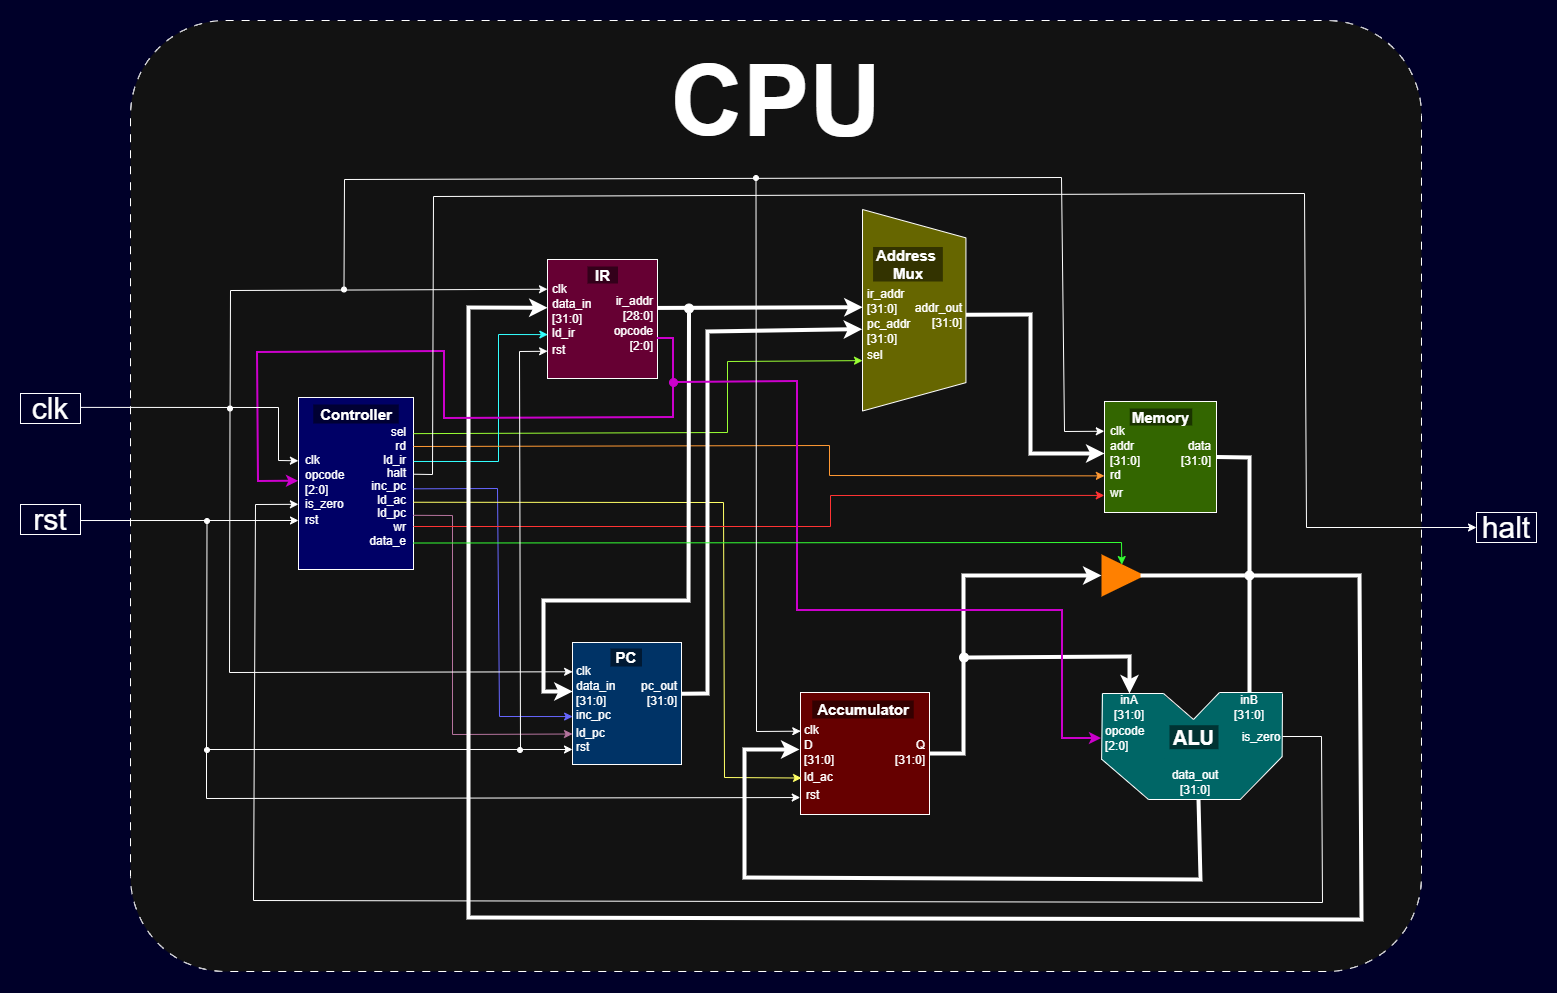
\includegraphics[width=\textwidth]{CPU.png} 
    \caption{Kiến trúc tổng thể và luồng dữ liệu của CPU}
    \label{fig:cpu_top_diagram}
\end{figure}

\textbf{Phân tích cấu trúc kết nối hệ thống:}

Nhìn vào Sơ đồ \ref{fig:cpu_top_diagram}, 
có thể thấy kiến trúc tổng thể của CPU được chia làm hai hệ thống 
mạng lưới dây dẫn biệt lập, hoạt động đan xen nhau:

\begin{itemize}
    \item \textbf{Đường dẫn dữ liệu (Datapath - Các đường bus 32-bit nét đậm):} 
    Đảm nhiệm việc vận chuyển mã lệnh, địa chỉ và toán hạng giữa các khối chức năng.
    \begin{itemize}
        \item \textbf{Định tuyến Địa chỉ (Address Routing):} Địa chỉ truy cập bộ nhớ được lựa chọn qua khối Address Mux. Trong pha Fetch, địa chỉ được cấp từ \texttt{PC}. Trong pha Execute, địa chỉ được cấp từ trường \texttt{ir\_addr} của \texttt{IR}.
        \item \textbf{Định tuyến Lệnh nhảy (Jump Routing):} Một nhánh của bus \texttt{ir\_addr} được nối trực tiếp vào ngõ vào \texttt{data\_in} của \texttt{PC}. Đây là đường dẫn dữ liệu phần cứng cốt lõi để thực thi lệnh rẽ nhánh không điều kiện (\texttt{JMP}).
        \item \textbf{Vòng lặp tính toán (ALU Execution Loop):} Mọi phép toán đều lấy thanh ghi \texttt{Accumulator} làm trung tâm. Toán hạng thứ nhất (\texttt{inA}) luôn được cấp từ ngõ ra của Accumulator, trong khi toán hạng thứ hai (\texttt{inB}) được lấy trực tiếp từ bus dữ liệu của \texttt{Memory}.
        \item \textbf{Lưu trữ dữ liệu (Store Path):} Khối đệm 3 trạng thái (Tristate Buffer) được đặt giữa Accumulator và bus bộ nhớ. Khi cần thực thi lệnh \texttt{STO}, cổng này mở ra, cho phép dữ liệu từ Accumulator chảy ngược lên bus chung để ghi vào bộ nhớ.
    \end{itemize}
    
    \item \textbf{Đường dẫn điều khiển (Control Path - Các đường tín hiệu 1-bit nét thanh):} 
    \begin{itemize}
        \item Khối \texttt{Controller} đóng vai trò là nhạc trưởng. Nó liên tục lắng nghe mã lệnh \texttt{opcode} từ \texttt{IR} và cờ \texttt{is\_zero} phản hồi từ \texttt{ALU}.
        \item Dựa trên Máy trạng thái 8 pha, \texttt{Controller} sẽ kích hoạt các tín hiệu điều khiển (như \texttt{sel, rd, wr, inc\_pc, ld\_ac...}) tới chân Enable của từng khối logic tại các nhịp clock tương ứng. Việc phân chia tín hiệu độc lập đảm bảo hệ thống vận hành tuần tự, không bao giờ xảy ra tình trạng đụng độ dữ liệu (Data Hazard) trên bus hệ thống.
    \end{itemize}
\end{itemize} 

% 3.2. Các khối chức năng
\subsection{Các khối chức năng}
% 3.2.1. Program Counter
%\subsubsection{Program Counter (PC)}
%Bộ đếm chương trình (Program Counter - PC) gồm một thanh ghi 32-bit có nhiệm vụ lưu trữ và cập nhật địa chỉ của câu lệnh tiếp theo sẽ được thực thi. 

\begin{figure}[H]
 \centering
 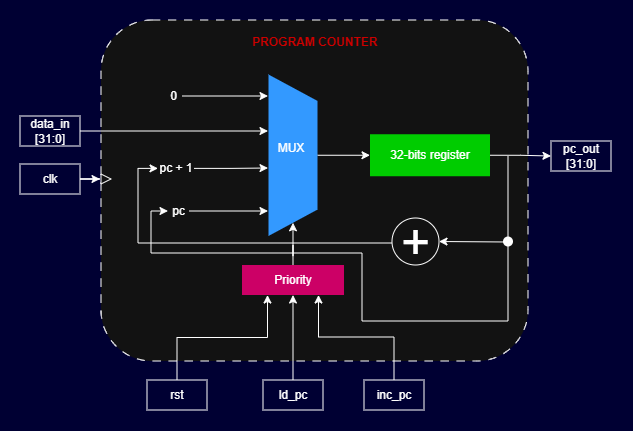
\includegraphics[width=0.8\textwidth]{PC.png} % Thay tên file sơ đồ khối PC vào đây
 \caption{Sơ đồ khối bộ đếm chương trình (PC) 32-bit}
 \label{fig:pc_32bit}
\end{figure}

\textbf{Nguyên lý hoạt động:}
Khối PC hoạt động đồng bộ theo xung lên của clk và output được chọn bởi một MUX đi kèm với một mạch ưu tiên logic. 
Khối sẽ thay đổi trạng thái dựa trên các tín hiệu điều khiển với mức độ ưu tiên từ cao xuống thấp như sau:

\begin{itemize}
 \item \textbf{Reset ($rst$):}Khi được kích hoạt, bộ đếm ngay lập tức bị xóa về giá trị 0 ($PC = 0$), đưa chương trình về trạng thái khởi tạo.
 \item \textbf{Nạp địa chỉ mới ($ld\_pc$):} Được sử dụng khi thực thi lệnh rẽ nhánh (như lệnh JMP). 
 PC sẽ nạp trực tiếp một địa chỉ 32-bit từ đầu vào ($PC = data\_in$).
 \item \textbf{Tăng bộ đếm ($inc\_pc$):} Ở trạng thái bình thường, bộ đếm sử dụng bộ cộng (Adder) 
 để tự động tăng giá trị hiện tại lên 1 đơn vị ($PC = PC + 1$), giúp CPU trỏ tới lệnh tiếp theo.
 \item \textbf{Giữ nguyên trạng thái:} Nếu không có tín hiệu nào trong ba tín hiệu trên được kích hoạt, PC sẽ duy trì giá trị địa chỉ hiện tại.
\end{itemize}

% 3.2.2. Address Mux
%\subsubsection{Address Mux}
%Khối đa hợp địa chỉ (Address Mux) là một mạch tổ hợp lựa chọn địa chỉ đi vào bộ nhớ (Memory) dựa theo chu kì hoạt động. 
Ngoài ra khối còn được thiết kế với tham số \textbf{width} (mặc định 32-bit), cho phép dễ dàng mở rộng không gian địa chỉ khi cần thiết.

\begin{figure}[H]
    \centering
    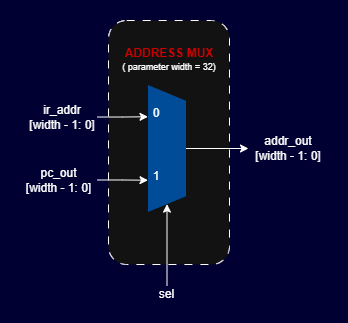
\includegraphics[width=0.7\textwidth]{Address_mux.png} 
    \caption{Sơ đồ khối bộ đa hợp địa chỉ (Address Mux)}
    \label{fig:address_mux}
\end{figure}

\textbf{Nguyên lý hoạt động:}
Khối Address Mux hoạt động dựa vào tín hiệu \textit{sel} từ khối Controller với logic hoạt động như sau:

\begin{itemize}
    \item \textbf{Giai đoạn nạp lệnh ($sel = 1$):} 
    \texttt{Address Mux} sẽ ưu tiên lựa chọn địa chỉ từ \texttt{PC} ($pc\_out$). 
    Lúc này địa chỉ của lệnh tiếp theo sẽ được đưa đến bộ nhớ để thực hiện quá trình lấy lệnh (Instruction Fetch).
    
    \item \textbf{Giai đoạn thực thi ($sel = 0$):} 
    \texttt{Address Mux} chuyển sang lựa chọn địa chỉ toán hạng từ \texttt{IR} ($ir\_addr$). 
    Việc này giúp CPU định vị được vị trí toán hạng để đưa vào tính toán.
\end{itemize}

% 3.2.3. ALU (Arithmetic Logic Unit)
\subsubsection{ALU (Arithmetic Logic Unit)}


Đơn vị số học và logic (ALU) là thành phần thực thi các phép toán cốt lõi của CPU. Mặc dù hệ thống sử dụng định dạng mã hóa lệnh 8-bit (3-bit Opcode và 5-bit Operand), nhưng khối ALU được thiết kế để xử lý dữ liệu với độ rộng thực tế là \textbf{32-bit}. Điều này cho phép máy tính thực hiện các phép tính trên dải giá trị lớn, đáp ứng tiêu chuẩn của các kiến trúc máy tính hiện đại.

\begin{figure}[H]
    \centering
    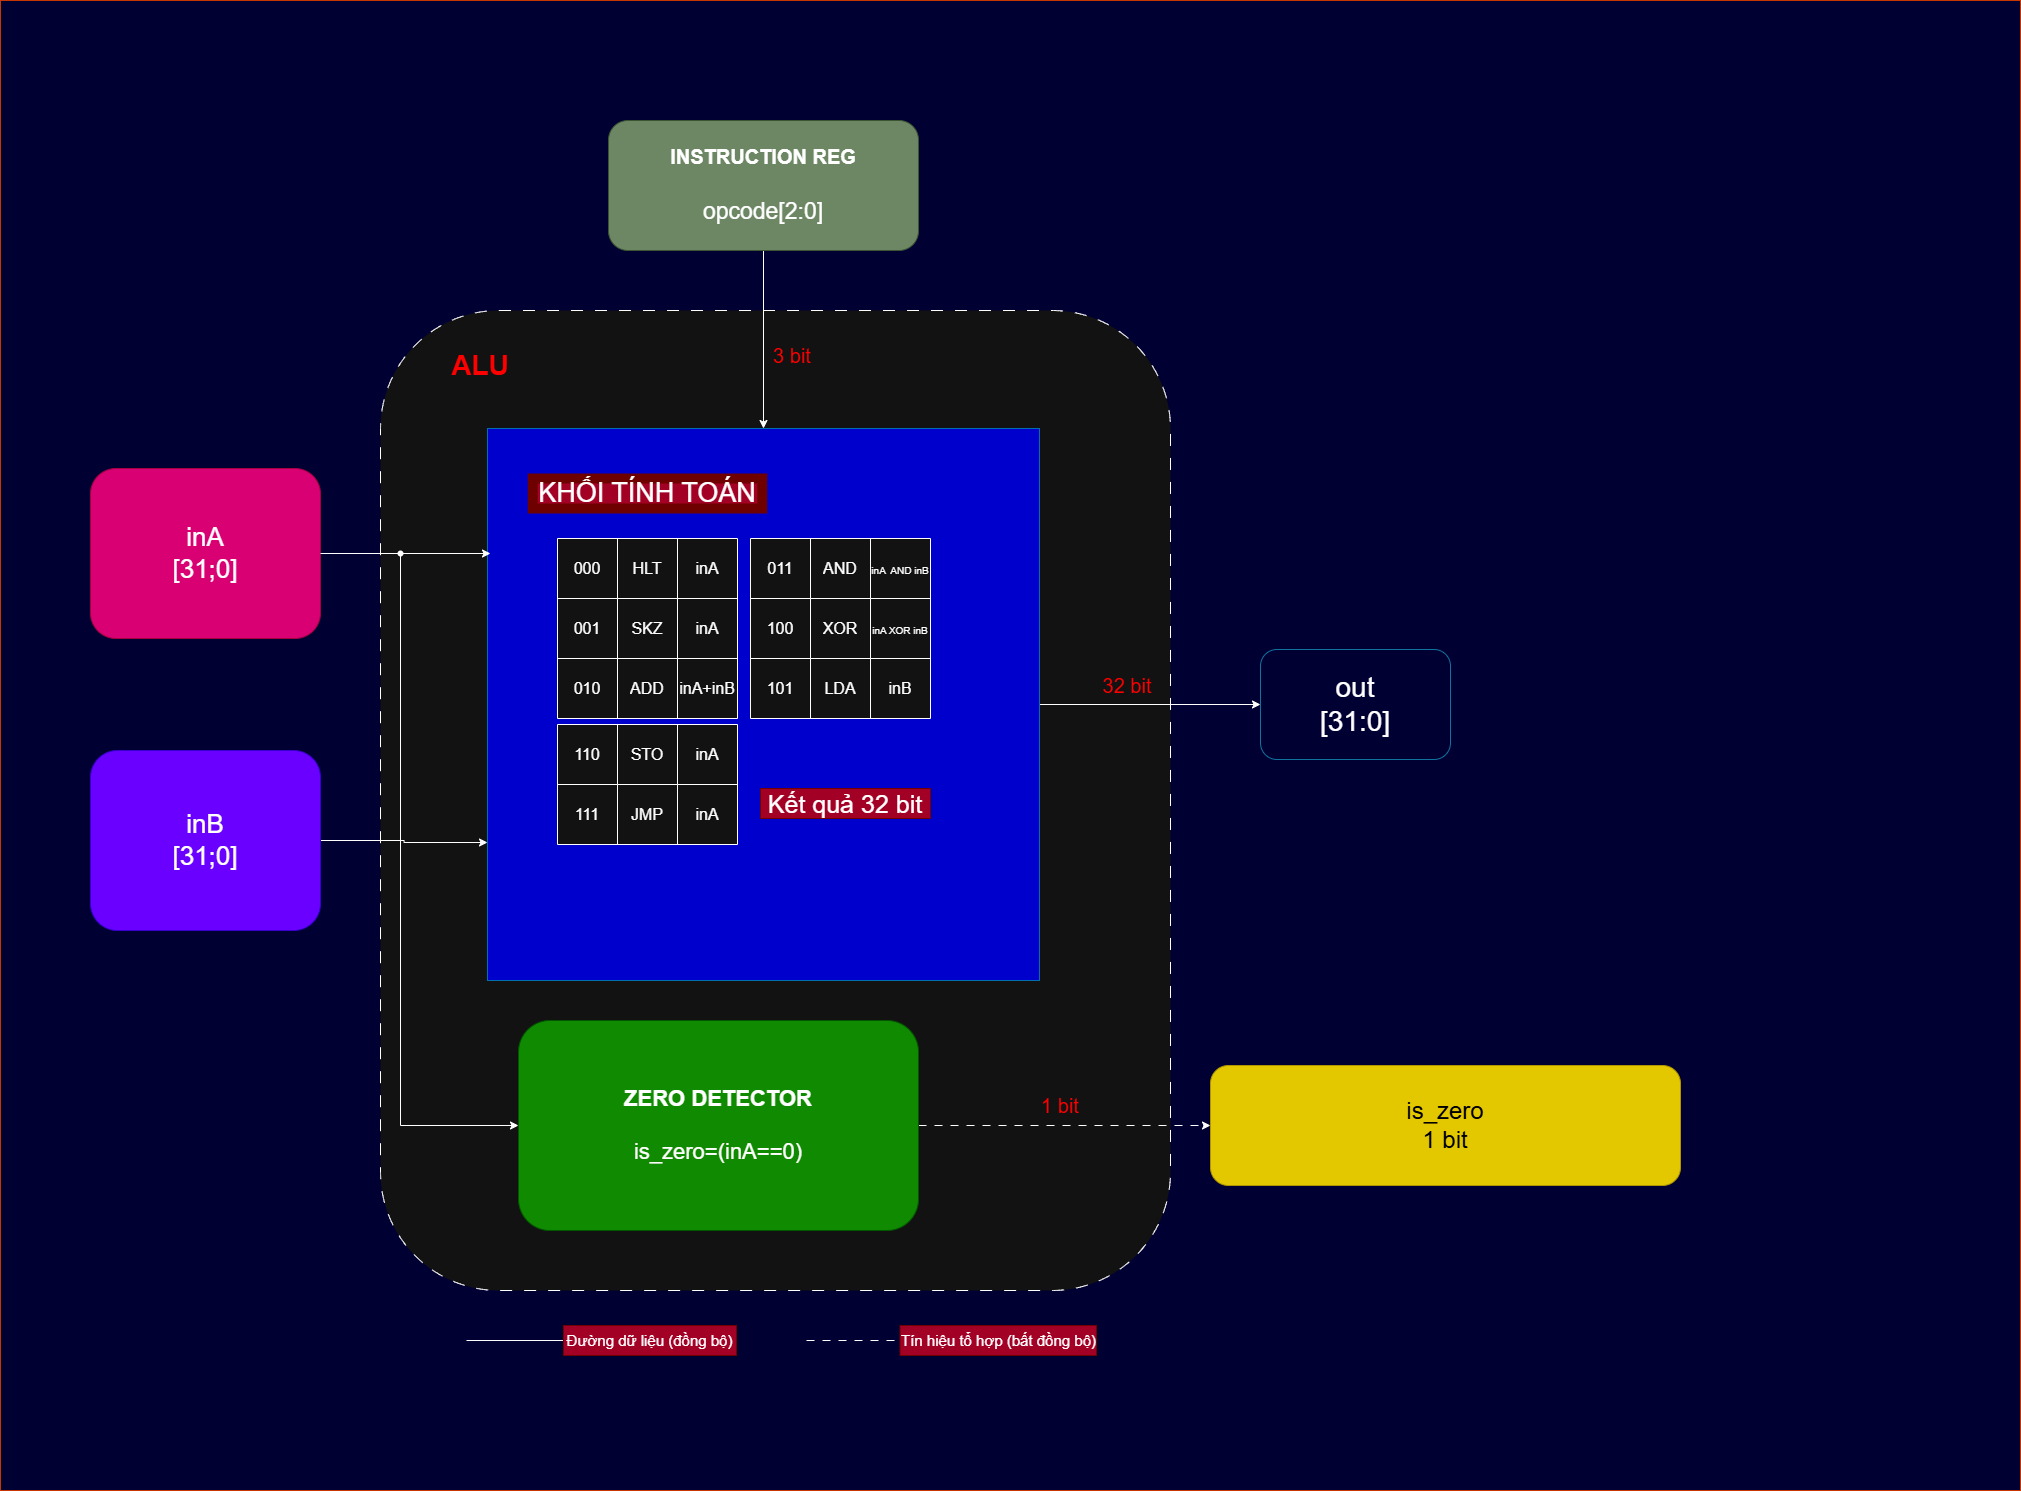
\includegraphics[width=0.9\textwidth]{ALU.png} 
    \caption{Sơ đồ khối tổng quát đơn vị ALU xử lý dữ liệu 32-bit}
    \label{fig:alu_32bit}
\end{figure}

\textbf{Nguyên lý thực thi các phép toán chi tiết:}
Dựa trên Opcode 3-bit từ khối điều khiển, ALU sẽ kích hoạt các mạch logic tương ứng để xử lý hai toán hạng 32-bit ($inA$ và $inB$):

\begin{itemize}
    \item \textbf{Phép cộng (ADD - Opcode 010):} 
    Thực hiện cộng đại số hai giá trị 32-bit. Kết quả $ALU\_Out = inA + inB$. Phép toán này sử dụng bộ cộng đầy đủ (Full Adder) 32-bit để xử lý dữ liệu từ Accumulator và bộ nhớ.
    
    \begin{figure}[H]
        \centering
        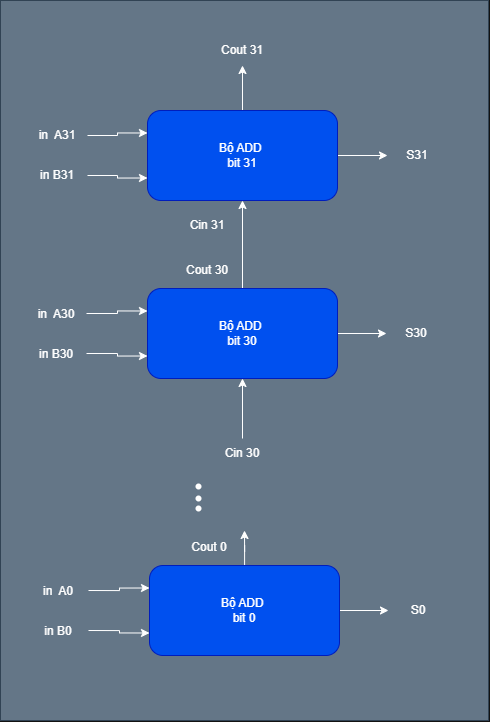
\includegraphics[width=0.8\textwidth]{add.png} % Thay tên file sơ đồ phép ADD vào đây
        \caption{Sơ đồ khối logic cho phép toán ADD 32-bit}
    \end{figure}

    \item \textbf{Phép logic AND (Opcode 011):} 
    Thực hiện phép toán bitwise AND giữa $inA$ và $inB$ trên toàn bộ 32 bit. Kết quả đầu ra chỉ bằng 1 tại các vị trí bit mà cả hai đầu vào đều bằng 1.
    
    \begin{figure}[H]
        \centering
        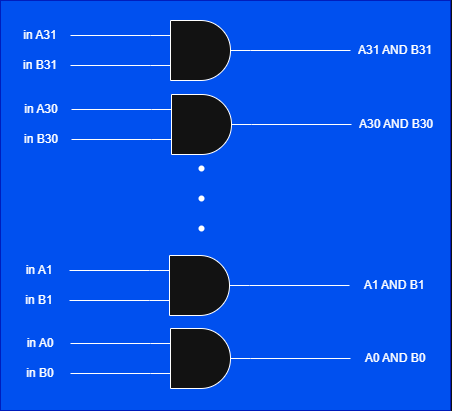
\includegraphics[width=0.9\textwidth]{and.png} % Thay tên file sơ đồ phép AND vào đây
        \caption{Sơ đồ khối logic cho phép toán AND 32-bit}
    \end{figure}

    \item \textbf{Phép logic XOR (Opcode 100):} 
    Thực hiện phép toán bitwise XOR giữa hai toán hạng 32-bit. Phép toán này đặc biệt hữu ích trong việc kiểm tra sự khác biệt hoặc đảo bit dữ liệu.
    
    \begin{figure}[H]
        \centering
        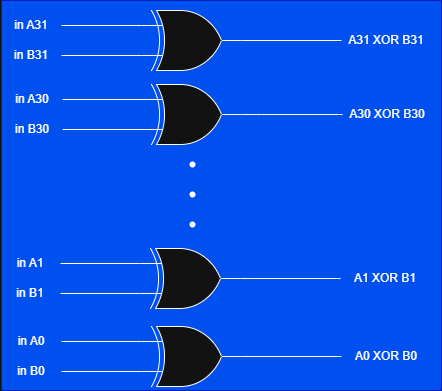
\includegraphics[width=0.6\textwidth]{xor.png} % Thay tên file sơ đồ phép XOR vào đây
        \caption{Sơ đồ khối logic cho phép toán XOR 32-bit}
    \end{figure}
\end{itemize}

\textbf{Tín hiệu Zero Flag ($is\_zero$):}
Một đầu ra quan trọng khác của ALU là tín hiệu $is\_zero$ được tính toán bất đồng bộ. Nếu toàn bộ 32 bit của kết quả đầu ra đều bằng 0, tín hiệu này sẽ được kéo lên mức logic 1. Đây là cơ sở để thực hiện lệnh nhảy có điều kiện \textbf{SKZ} (Skip if Zero).

% 3.2.4. Controller
%\subsubsection{Controller}
%Khối điều khiển (Controller) tiếp nhận, xử lý và điều phối các tín hiệu kích hoạt cho quá trình nạp lệnh và thực thi lệnh. 
Controller được thiết kế đồng bộ theo xung lên của (\texttt{clk}) và sử dụng máy trạng thái hữu hạn (Finite State Machine - FSM) 
gồm 8 pha hoạt động liên tục.

\begin{figure}[H]
    \centering
    % Đảm bảo file ảnh nằm cùng thư mục với file .tex. Thay đổi tên file nếu cần.
    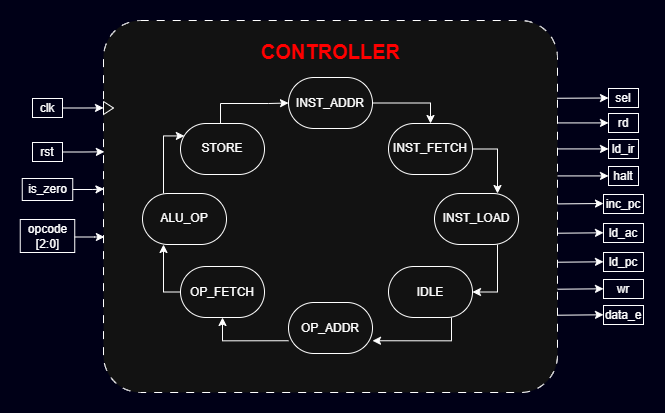
\includegraphics[width=0.75\textwidth]{Controller.png} 
    \caption{Sơ đồ khối và máy trạng thái 8 pha của Controller}
    \label{fig:controller_diagram}
\end{figure}

\textbf{Các tín hiệu bao gồm:}

\begin{itemize}
    \item \textbf{Tín hiệu vào (Inputs): }
    \begin{itemize}
        \item \textbf{\texttt{opcode [2:0]}: } Mã lệnh 3-bit nhận từ khối \texttt{IR}. 
        Dữ liệu được Controller giải mã và quyết định thao tác thực thi trong các pha tiếp theo.
        \item \textbf{\texttt{is\_zero}: } Cờ trạng thái từ khối ALU, tích cực khi kết quả tính toán bằng 0. 
        Tín hiệu này kết hợp với mã lệnh \texttt{SKZ} để quyết định việc rẽ nhánh.
        \item \textbf{\texttt{clk}: } Xung nhịp đồng bộ.
        \item \textbf{\texttt{rst}: } Đưa Controller về trạng thái ban đầu.
    \end{itemize}
    
    \item \textbf{Tín hiệu ra (Outputs):}
    \begin{itemize}
        \item \textbf{Nhóm Định tuyến và Bộ nhớ:} \texttt{sel} (Chọn địa chỉ từ \texttt{PC} hoặc \texttt{IR}), \texttt{rd} (Cho phép đọc từ Memory), 
        \texttt{wr} (Cho phép ghi vào Memory), \texttt{data\_e} (Cho phép dữ liệu từ Accumulator đi vào bus).
        \item \textbf{Nhóm Thanh ghi:} \texttt{ld\_ir} (Cho phép lệnh đi vào IR), \texttt{ld\_ac} (Cho dữ liệu đi vào Accumulator), 
        \texttt{ld\_pc} (Cho phép nạp địa chỉ vào PC), \texttt{inc\_pc} (Tăng giá trị PC).
        \item \textbf{Tín hiệu dừng:} \texttt{halt} (Dừng toàn bộ hoạt động của CPU).
    \end{itemize}
\end{itemize}

\textbf{Nguyên lý hoạt động của Máy trạng thái (FSM):}

Hệ thống hoạt động theo một vòng lặp khép kín gồm 8 pha, 
bắt đầu từ trạng thái reset là \texttt{INST\_ADDR}. Quá trình được chia làm hai giai đoạn chính:

\begin{enumerate}
    \item \textbf{Giai đoạn Nạp lệnh (Fetch Phase):} Bao gồm 4 trạng thái đầu tiên: \texttt{INST\_ADDR}, \texttt{INST\_FETCH}, \texttt{INST\_LOAD}, và \texttt{IDLE}. 
    \begin{itemize}
        \item Trong suốt giai đoạn này, tín hiệu \texttt{sel = 1} được giữ cố định để địa chỉ đi từ PC tới bộ nhớ.
        \item Bộ nhớ được phép đọc (\texttt{rd = 1}) và lệnh được đưa vào IR (\texttt{ld\_ir = 1}) ở các pha tương ứng.
    \end{itemize}
    
    \item \textbf{Giai đoạn Thực thi (Execute Phase):} Bao gồm 4 trạng thái cuối: \texttt{OP\_ADDR}, \texttt{OP\_FETCH}, \texttt{ALU\_OP}, và \texttt{STORE}.
    \begin{itemize}
        \item Tín hiệu \texttt{sel} chuyển về \texttt{0} để sử dụng phần địa chỉ chứa trong câu lệnh hiện tại.
        \item Tại \texttt{OP\_ADDR}, tín hiệu \texttt{inc\_pc} được kích hoạt bằng \texttt{1} để trỏ sẵn PC tới lệnh kế tiếp.
        \item Các ngõ ra trong các pha tiếp theo phụ thuộc vào bộ giải mã lệnh (\texttt{opcode}):
        \begin{itemize}
            \item Các lệnh tính toán (\texttt{ADD, AND, XOR, LDA}) sẽ kích hoạt \texttt{rd = 1} để lấy toán hạng và \texttt{ld\_ac = 1} tại pha \texttt{STORE} để lưu kết quả.
            \item Lệnh nhảy (\texttt{SKZ}) sẽ kiểm tra cờ \texttt{zero}. Nếu \texttt{zero = 1}, 
            tín hiệu \texttt{inc\_pc} sẽ được kích hoạt thêm một lần nữa tại pha \texttt{ALU\_OP}.
            \item Lệnh lưu dữ liệu (\texttt{STO}) sẽ kích hoạt \texttt{wr = 1} và \texttt{data\_e = 1} tại pha \texttt{STORE} để đẩy dữ liệu từ Accumulator vào bộ nhớ.
            \item Lệnh dừng (\texttt{HLT}) kích hoạt tín hiệu \texttt{halt = 1} ngay tại pha \texttt{OP\_ADDR}.
        \end{itemize}
    \end{itemize}
\end{enumerate}

% 3.2.5. . Register (Accumulator / Instruction Register)
\subsubsection{Register (Accumulator / Instruction Register)}
\input{phan3251.tex}
%\input{phan3252.tex}

% 3.2.6. Memory
%\subsubsection{Memory}
%Bộ nhớ (Memory) đóng vai trò là kho lưu trữ trung tâm cho cả lệnh chương trình 
và dữ liệu. 
Bộ nhớ sử dụng cổng dữ liệu lưỡng cực (Single bidirectional data port) có chức năng đọc và ghi, đảm bảo bộ nhớ không đọc và ghi cùng lúc.

\begin{figure}[H]
    \centering
    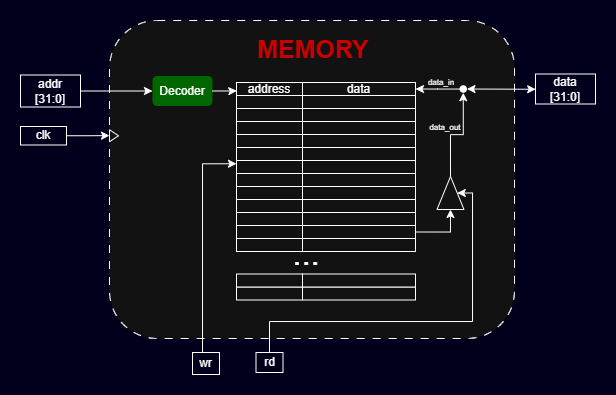
\includegraphics[width=0.9\textwidth]{Memory.png} 
    \caption{Sơ đồ khối Memory 32-bit}
    \label{fig:memory_internal}
\end{figure}

\textbf{Nguyên lý hoạt động:}
Khối Memory hoạt động đồng bộ với xung lên của clk và được quản lý bởi 
các tín hiệu điều khiển từ Controller. Thành phần của khối bao gồm:

\begin{itemize}
    \item \textbf{Giải mã địa chỉ (Address Decoding):} 
    Địa chỉ 32-bit từ ngõ vào sẽ đi qua khối Decoder. 
    giải mã vị trí hàng và cột trong mảng ô nhớ để chuẩn bị cho các thao tác truy xuất dữ liệu.
    
    \item \textbf{Ghi dữ liệu ($wr = 1$):} 
    Quá trình ghi diễn ra đồng bộ tại xung lên của clk. Khi tín hiệu \textit{wr} 
    được kích hoạt, dữ liệu từ cổng \textit{data} bên ngoài sẽ đi theo nhánh 
    \textit{data\_in} để đi vào ô nhớ đã được chọn bởi bộ giải mã.
    
    \item \textbf{Đọc dữ liệu và Trở kháng cao ($rd = 1$):} 
    Dữ liệu từ ô nhớ được đưa ra đường \textit{data\_out} 
    dẫn tới bộ đệm 3 trạng thái. 
    \begin{itemize}
        \item Khi $rd = 1$: Bộ đệm mở cho phép dữ liệu từ 
            \textit{data\_out} đi ra cổng giao tiếp bên ngoài.
        \item Khi $rd = 0$: 
        Bộ đệm sẽ đưa đầu ra về trạng thái trở kháng cao ($Z$), giúp "ngắt kết nối" bộ nhớ khỏi bus dữ liệu chung.
    \end{itemize}
\end{itemize}

    \newpage

    \section{HIỆN THỰC}

% 4.1. Cấu trúc tổng thể dự án
\subsection{Cấu trúc tổng thể dự án}

Dự án được tổ chức theo mô hình phân cấp module, mỗi khối chức năng tương ứng với một file Verilog riêng biệt, 
kèm theo các file testbench riêng biệt để kiểm thử từng khối trước khi tích hợp vào hệ thống.

\textbf{Sơ đồ tổ chức thư mục dự án:}
\begin{verbatim}
RISC_CPU/
|
+-- src/                        # Ma nguon thiet ke chinh
|   +-- ALU.v                   # Khoi ALU (8 phep toan, 32-bit)
|   +-- Accumulator.v           # Khoi Accumulator Register
|   +-- program_counter.v       # Khoi Program Counter (PC)
|   +-- address_mux.v           # Khoi Address Mux
|   +-- Instruction_Register.v  # Khoi Instruction Register (IR)
|   +-- memory.v                # Khoi Memory 
|   +-- controller.v            # Khoi Controller
|   +-- CPU_Top.v               # File Top-level tich hop toan he thong
|
+-- tb/                         # Testbench kiem thu tung khoi
|   +-- ALU_tb.v                # Testbench cho ALU
|   +-- Accumulator_tb.v        # Testbench cho Accumulator Register
|   +-- ...                     # Cac testbench tuong ung khac
|   +-- CPU_Top_tb.v            # Testbench toan he thong
|
+-- sim/                        # Ket qua mo phong
    +-- waveform/               # File waveform (.vcd) tu Vivado
\end{verbatim}

\textbf{Vai trò của các thành phần cốt lõi:}

\begin{table}[H]
\centering
\caption{Danh mục vai trò các module trong hệ thống CPU}
\renewcommand{\arraystretch}{1.5}
\begin{tabularx}{\textwidth}{|l|>{\raggedright\arraybackslash}X|}
\hline
\rowcolor[HTML]{EFEFEF} 
\textbf{Tên File} & \textbf{Vai trò trong hệ thống} \\ \hline
\texttt{ALU.v} & Thực thi 8 phép toán số học và logic dựa trên Opcode 3-bit, xuất kết quả 32-bit và tín hiệu \texttt{is\_zero}. \\ \hline
\texttt{Accumulator.v} & Lưu trữ kết quả trung gian từ ALU, hỗ trợ reset đồng bộ và cập nhật dữ liệu khi \texttt{load\_en = 1}. \\ \hline
\texttt{program\_counter.v} & Bộ đếm địa chỉ lệnh 32-bit, hỗ trợ tăng tuần tự hoặc nạp địa chỉ nhảy khi thực hiện lệnh \texttt{JMP}. \\ \hline
\texttt{address\_mux.v} & Lựa chọn giữa địa chỉ lệnh (từ PC) và địa chỉ toán hạng (từ IR) dựa trên tín hiệu điều khiển \texttt{sel}. \\ \hline
\texttt{Instruction\_Register.v} & Lưu trữ mã lệnh nạp từ Memory, thực hiện tách Opcode cho Controller và địa chỉ cho Address Mux. \\ \hline
\texttt{memory.v} & Đơn vị lưu trữ lệnh và dữ liệu, hỗ trợ đọc/ghi thông qua cổng dữ liệu song hướng (\textit{bidirectional port}). \\ \hline
\texttt{controller.v} & Khối điều khiển trung tâm sử dụng FSM 8 trạng thái để phát động các tín hiệu điều khiển toàn hệ thống. \\ \hline
\texttt{CPU\_Top.v} & Module cấp cao nhất thực hiện kết nối tất cả các khối chức năng thành một kiến trúc CPU hoàn chỉnh. \\ \hline
\end{tabularx}
\end{table}

% 4.2. Hiện thực Program Counter
\subsection{Hiện thực Program Counter}

Bộ đếm chương trình (Program Counter - PC) đóng vai trò là con trỏ lệnh, quản lý địa chỉ của lệnh sẽ được thực thi tiếp theo trong bộ nhớ. Khối này đảm bảo luồng thực thi của chương trình được duy trì liên tục hoặc thay đổi linh hoạt thông qua các lệnh nhảy.

\begin{lstlisting}[language=Verilog, caption={Ma nguon hien thuc module Program Counter}]
module program_counter (
    input             clk,      // Xung clock he thong
    input             rst,      // Reset dong bo (active high)
    input             ld_pc,    // Tin hieu nap dia chi moi (lenh JMP)
    input             inc_pc,   // Tin hieu tang dia chi (Fetch/SKZ)
    input      [31:0] d_in,     // Dia chi nap vao tu Instruction Register
    output reg [31:0] pc_out    // Dia chi chuong trinh hien tai
);

    // Hoat dong tai canh len cua clock (Sequential Logic)
    always @(posedge clk) begin
        if (rst) begin
            pc_out <= 32'b0;    // Reset bo dem ve dia chi goc 0
        end
        else if (ld_pc) begin
            pc_out <= d_in;     // Uu tien nap dia chi nhay (JMP)
        end
        else if (inc_pc) begin
            pc_out <= pc_out + 1; // Tang dia chi len 1 don vi
        end
        // Neu ld_pc = 0 va inc_pc = 0, pc_out duy tri trang thai cu
    end

endmodule
\end{lstlisting}

\textbf{Mô tả logic xử lý :}
\begin{itemize}
    \item \textbf{Cơ chế tăng địa chỉ:} Chân \texttt{inc\_pc} giờ đây được điều khiển bởi trạng thái \texttt{STORE} của Controller, giúp PC luôn trỏ sẵn sang lệnh tiếp theo ngay khi lệnh hiện tại kết thúc.
    \item \textbf{Xử lý lệnh rẽ nhánh:} Khi thực hiện lệnh \texttt{SKZ} (Skip if Zero), nếu cờ \texttt{is\_zero} bật, Controller sẽ phát thêm một xung \texttt{inc\_pc} bổ sung, giúp bộ đếm nhảy qua (skip) một địa chỉ lệnh.
\end{itemize}

% 4.3. Hiện thực Address Mux
\subsection{Hiện thực Address Mux}

Khối chọn địa chỉ (Address Mux) là một bộ dồn kênh (Multiplexer) đóng vai trò điều phối luồng địa chỉ truy cập vào bộ nhớ. Tùy thuộc vào giai đoạn của chu kỳ lệnh, bộ chọn này sẽ quyết định lấy địa chỉ từ Program Counter (để nạp lệnh) hay từ Instruction Register (để truy cập toán hạng).

\begin{lstlisting}[language=Verilog, caption={Ma nguon hien thuc module Address Mux}]
module address_mux #(
    parameter WIDTH = 32  // Do rong mac dinh la 32-bit
)(
    input      [WIDTH-1:0] pc_addr,  // Dia chi tu Program Counter
    input      [WIDTH-1:0] ir_addr,  // Dia chi tu Instruction Register
    input                  sel,      // Tin hieu chon tu Controller
    output reg [WIDTH-1:0] addr_out  // Dia chi xuat ra bo nho
);

    // Logic chon dia chi (Combinational Logic)
    always @(*) begin
        if (sel)
            addr_out = pc_addr;      // Giai doan nap lenh (Fetch)
        else
            addr_out = ir_addr;      // Giai doan thuc thi (Execute)
    end

endmodule
\end{lstlisting}

\textbf{Mô tả logic xử lý:}
\begin{itemize}
    \item \textbf{Logic tổ hợp thuần túy:} Khối \texttt{always @(*)} đảm bảo \texttt{addr\_out} phản hồi tức thời với sự thay đổi của các ngõ vào mà không cần chờ xung nhịp clock. Điều này cực kỳ quan trọng để đảm bảo địa chỉ bộ nhớ ổn định ngay khi tín hiệu điều khiển \texttt{sel} được thiết lập.
    \item \textbf{Cơ chế điều phối luồng:} 
        \begin{itemize}
            \item Khi \texttt{sel = 1}: Hệ thống đang ở trạng thái nạp lệnh (Fetch), địa chỉ từ \texttt{pc\_addr} được đưa ra để truy xuất mã máy.
            \item Khi \texttt{sel = 0}: Hệ thống chuyển sang giai đoạn thực thi (Execute), địa chỉ trích xuất từ lệnh (\texttt{ir\_addr}) được ưu tiên để truy xuất dữ liệu toán hạng.
        \end{itemize}
    \item \textbf{Tính linh hoạt:} Việc sử dụng \texttt{parameter WIDTH} cho phép module dễ dàng tái sử dụng cho các kiến trúc CPU có độ rộng bus địa chỉ khác nhau (như 16-bit hoặc 64-bit) mà không cần chỉnh sửa mã nguồn cốt lõi.
\end{itemize}

% 4.4. Hiện thực ALU
\subsection{Hiện thực ALU}


\begin{lstlisting}[language=Verilog, caption={ALU}, label={lst:alu_code}]
module ALU (
    input  [31:0] inA,      
    input  [31:0] inB,      
    input  [2:0]  opcode,   
    output reg [31:0] out,  
    output        is_zero   
);

    localparam HLT = 3'b000, SKZ = 3'b001, ADD = 3'b010, AND = 3'b011,
               XOR = 3'b100, LDA = 3'b101, STO = 3'b110, JMP = 3'b111;

    always @(*) begin
        case (opcode)
            HLT, SKZ, JMP, STO : out = inA; 
            ADD : out = inA + inB;
            AND : out = inA & inB;
            XOR : out = inA ^ inB;
            LDA : out = inB;
            default: out = inA;
        endcase
    end

  
    assign is_zero = (inA == 32'b0); 

endmodule
\end{lstlisting}

\textbf{Mô tả logic xử lý chi tiết:}
\begin{itemize}
    \item \textbf{Nhóm lệnh tính toán (ADD, AND, XOR):} ALU thực hiện trực tiếp các phép toán tương ứng giữa hai toán hạng 
    \texttt{inA} và \texttt{inB}. Việc tổng hợp các toán tử \texttt{+}, \texttt{\&}, \texttt{\textasciicircum} sẽ tự động tạo ra các bộ cộng và cổng logic phần cứng tương ứng.
    \item \textbf{Lệnh nạp dữ liệu (LDA):} Dữ liệu từ ngõ vào \texttt{inB} được truyền trực tiếp ra \texttt{out} để chuẩn bị nạp vào thanh ghi Accumulator.
    \item \textbf{Nhóm lệnh truyền thẳng (HLT, SKZ, JMP, STO):} Các lệnh này không yêu cầu tính toán. 
    ALU sẽ đóng vai trò như một đường dẫn trong suốt, 
    truyền trực tiếp giá trị của \texttt{inA} ra ngõ \texttt{out}. 
    Việc gom nhóm các case này giúp phần mềm tổng hợp tối ưu hóa bộ dồn kênh (MUX).
    \item \textbf{Tín hiệu cờ \texttt{is\_zero}:} Tín hiệu này được thiết kế bằng lệnh \texttt{assign} nằm ngoài khối \texttt{always},
     giúp nó hoạt động hoàn toàn độc lập và bất đồng bộ. 
     Tín hiệu này giám sát liên tục ngõ vào \texttt{inA}; nếu $\texttt{inA} = 0$, cờ sẽ lập tức bật lên mức 1.
\end{itemize}

% 4.5. Hiện thực Controller
\subsection{Hiện thực Controller}

Khối điều khiển là thành phần quan trọng nhất trong kiến trúc CPU, đóng vai trò điều phối toàn bộ các khối chức năng khác thông qua việc giải mã mã lệnh (Opcode). Module này được hiện thực bằng máy trạng thái hữu hạn (FSM) với 8 pha (Phases) tương ứng với một chu kỳ lệnh đầy đủ.

\textbf{Mã nguồn Verilog hiện thực khối điều khiển:}

\begin{lstlisting}[language=Verilog, caption={Ma nguon hien thuc khoi dieu khien trung tam (Controller)}]
module controller (
    input clk, rst,
    input [2:0] opcode,
    input is_zero,          // Tin hieu tu ALU de xu ly lenh SKZ
    output reg sel, rd, ld_ir, halt, inc_pc, ld_ac, ld_pc, wr, data_e,
    output [2:0] debug_state
);
    reg [2:0] state, next_state;
    
    // Khai bao 8 trang thai cua chu ky lenh (8-Phase)
    parameter INST_ADDR = 3'd0, INST_FETCH = 3'd1, INST_LOAD = 3'd2, IDLE = 3'd3,
              OP_ADDR = 3'd4, OP_FETCH = 3'd5, ALU_OP = 3'd6, STORE = 3'd7;

    // Dinh nghia tap lenh (Instruction Set Architecture)
    localparam HLT=3'b000, SKZ=3'b001, ADD=3'b010, AND=3'b011, 
               XOR=3'b100, LDA=3'b101, STO=3'b110, JMP=3'b111;

    // 1. Bo nho trang thai (State Register) - Reset dong bo
    always @(posedge clk) begin
        if (rst) state <= INST_ADDR;
        else     state <= next_state;      
    end
    assign debug_state = state;

    // 2. Logic chuyen trang thai ke tiep
    always @(*) begin
        next_state = state + 1; // Tu dong chuyen tuan tu qua 8 buoc
    end

    // 3. Logic dieu khien dau ra (Output Logic)
    always @(*) begin
        // Gan gia tri mac dinh de tranh tao ra mach chot (latches) khong mong muon
        sel=0; rd=0; ld_ir=0; halt=0; inc_pc=0; ld_ac=0; ld_pc=0; wr=0; data_e=0;

        case(state)
            INST_ADDR:  sel = 1;
            INST_FETCH: begin sel = 1; rd = 1; end
            INST_LOAD:  begin sel = 1; rd = 1; ld_ir = 1; end
            IDLE:       begin sel = 1; rd = 1; ld_ir = 1; end
            OP_ADDR:    begin 
                sel = 0; 
                if (opcode == HLT) halt = 1; 
            end
            OP_FETCH:   begin 
                if (opcode == ADD || opcode == AND || opcode == XOR || opcode == LDA) rd = 1; 
            end
            ALU_OP:     begin
                if (opcode == ADD || opcode == AND || opcode == XOR || opcode == LDA) rd = 1;
                if (opcode == SKZ && is_zero) inc_pc = 1;
                if (opcode == JMP) ld_pc = 1;
                if (opcode == STO) data_e = 1;
            end
            STORE:      begin
                inc_pc = 1; // Luon tang PC tai buoc cuoi de tro sang lenh moi
                if (opcode == ADD || opcode == AND || opcode == XOR || opcode == LDA) begin
                    rd = 1; ld_ac = 1;
                end
                if (opcode == JMP) ld_pc = 1;
                if (opcode == STO) begin wr = 1; data_e = 1; end
            end
        endcase
    end
endmodule
\end{lstlisting}

\textbf{Mô tả logic xử lý:}
\begin{itemize}
    \item \textbf{Phân kỳ chu kỳ máy:} CPU vận hành dựa trên chu kỳ cố định 8 bước. Bốn trạng thái đầu thực hiện việc nạp lệnh (\textit{Instruction Fetch}) từ bộ nhớ vào thanh ghi lệnh (IR). Bốn trạng thái sau thực hiện việc giải mã và thực thi (\textit{Execute}) tùy theo Opcode.
    \item \textbf{Cơ chế nạp và lưu trữ:} Các tín hiệu cập nhật thanh ghi như \texttt{ld\_ac} và tín hiệu ghi bộ nhớ \texttt{wr} được đặt tại trạng thái cuối cùng (\texttt{STORE}). Điều này đảm bảo các phép tính toán tại ALU hoặc việc truyền dữ liệu trên Bus đã ổn định trước khi được chốt giá trị.
    \item \textbf{Điều phối Bus hệ thống:} Tín hiệu \texttt{data\_e} điều khiển cổng đệm ba trạng thái, đảm bảo CPU chỉ chiếm quyền ghi lên Bus dữ liệu khi thực hiện lệnh \texttt{STO}, tránh tình trạng xung đột dữ liệu (\textit{Bus contention}).
    \item \textbf{Xử lý lệnh rẽ nhánh:} Logic điều khiển cho phép thực hiện lệnh nhảy cách (\texttt{SKZ}) bằng cách kiểm tra cờ \texttt{is\_zero} và phát động thêm một xung \texttt{inc\_pc} bổ sung, giúp bỏ qua lệnh kế tiếp trong bộ nhớ.
\end{itemize}

% 4.6. Hiện thực Register
\subsection{Hiện thực Register}
\subsubsection{Hiện thực Accumulator Register}


\begin{lstlisting}[language=Verilog, caption={Accumulator Register}, label={lst:accum_code}]
module Accumulator (
    input         clk,        
    input         rst,        
    input         load_en,    
    input  [31:0] D,          
    output reg [31:0] Q     
);

    
    always @(posedge clk) begin
        if (rst) begin
            Q <= 32'b0;          
        end 
        else if (load_en) begin
            Q <= D;              
        end
        
    end

endmodule
\end{lstlisting}

\textbf{Mô tả logic xử lý:}
\begin{itemize}
    \item \textbf{Đồng bộ hóa tuyệt đối:} Khối \texttt{always} chỉ nhạy với xung lên clk. 
    Tín hiệu \texttt{rst} được kiểm tra ngay bên trong cấu trúc điều kiện của khối \texttt{always}, 
    đảm bảo mạch chỉ thực hiện việc xóa dữ liệu (\texttt{Q <= 0}) khi có xung clock tác động (Reset đồng bộ).
    \item \textbf{Truyền dữ liệu:} Khi tín hiệu \texttt{load\_en} ở mức logic 0, \
    thanh ghi tự động duy trì trạng thái cũ.
\end{itemize}
%\subsubsection{Hiện thực Instruction Register (IR)}
\begin{lstlisting}[language=Verilog, caption={Instruction Register}]
module instruction_reg (
    input             clk,      // Xung clock he thong
    input             rst,      // Reset dong bo 
    input             ld_ir,    // Tin hieu cho phep nap lenh tu Controller
    input      [31:0] data_in,  // Du lieu lenh tu Bus bo nho
    output reg [2:0]  opcode,   // 3-bit ma lenh 
    output reg [28:0] addr      // Dia chi bo nho di kem lenh
);

    // Instruction Register hoat dong dong bo theo canh len cua clock
    always @(posedge clk) begin
        if (rst) begin
            // Khoi tao gia tri ve 0 khi co tin hieu reset
            opcode <= 3'b000;
            addr   <= 29'b0;
        end
        else if (ld_ir) begin
            // Nap du lieu tu Bus vao thanh ghi khi ld_ir duoc kich hoat
            opcode <= data_in[31:29]; 
            addr   <= data_in[28:0];  
        end
    end

endmodule
\end{lstlisting}

\textbf{Mô tả logic xử lý:}
\begin{itemize}
    \item \textbf{Đồng bộ hóa tuyệt đối:} Khối \texttt{always} theo xung lên của clk. 
    Tín hiệu \texttt{rst} được kiểm tra ngay bên trong cấu trúc điều kiện của khối \texttt{always} thực hiện việc xóa dữ liệu (\texttt{opcode <= 0, addr <= 0}) theo xung clk (Reset đồng bộ).
    \item \textbf{Truyền dữ liệu:} Khi tín hiệu enable \texttt{ld\_ir} ở mức logic 0, 
    thanh ghi tự động duy trì trạng thái cũ. 
\end{itemize}

% 4.7. Hiện thực Memory
\subsection{Hiện thực Memory}


Khối bộ nhớ được thiết kế theo kiến trúc Von Neumann, đóng vai trò lưu trữ chung cho cả tập lệnh (Instruction) và dữ liệu (Data). Module tuân thủ nghiêm ngặt các yêu cầu kỹ thuật về độ rộng dữ liệu 32-bit và sử dụng cổng giao tiếp song hướng để tối ưu hóa Bus hệ thống.

\textbf{Mã nguồn Verilog hiện thực module Memory:}

\begin{lstlisting}[language=Verilog, caption={Ma nguon hien thuc khoi Bo nho (Memory)}]
module memory (
    input             clk,      // Xung clock he thong
    input      [31:0] addr,     // Bus dia chi 32-bit
    input             rd,       // Tin hieu cho phep doc (Active High)
    input             wr,       // Tin hieu cho phep ghi (Active High)
    inout      [31:0] data      // Cong du lieu song huong (Single bidirectional port)
);

    // Khai bao mang bo nho (256 o nho, moi o 32-bit)
    reg [31:0] ram [0:255];
    
    // Thanh ghi dem de giu du lieu sau khi doc tu RAM
    reg [31:0] data_out;

    // Thiet ke Single bidirectional data port bang buffer 3 trang thai
    // Ngon ngu Verilog su dung trang thai tro khang cao 'bz de giai phong Bus
    assign data = (rd && !wr) ? data_out : 32'bz;

    // Hoat dong dong bo: Thuc hien doc/ghi tai canh len cua xung clock (clk)
    always @(posedge clk) begin
        // Kiem soat logic: Khong cho phep doc va ghi cung mot luc
        if (wr && !rd) begin
            ram[addr[7:0]] <= data;      // Thao tac Ghi du lieu vao RAM
        end
        else if (rd && !wr) begin
            data_out <= ram[addr[7:0]];  // Thao tac Doc du lieu tu RAM ra dem
        end
    end

endmodule
\end{lstlisting}

\textbf{Mô tả logic xử lý :}
\begin{itemize}
    \item \textbf{Cổng song hướng (Inout):} Sử dụng một cổng duy nhất cho cả hai chiều dữ liệu. Khi tín hiệu \texttt{rd} và \texttt{wr} đều bằng 0 hoặc khi đang ở chế độ ghi, cổng dữ liệu được đặt ở trạng thái trở kháng cao (\texttt{Hi-Z}) để tránh xung đột điện áp trên đường Bus chung.
    \item \textbf{Độ phân giải địa chỉ:}CPU sử dụng 5-bit toán hạng tương ứng với 32 ô nhớ khả dụng. Tuy nhiên, trong quá trình hiện thực, nhóm đã quyết định mở rộng không gian bộ nhớ lên 256 ô nhớ bằng cách sử dụng 8-bit thấp của bus địa chỉ 32-bit (\texttt{addr[7:0]}). Quyết định này xuất phát từ các lý do kỹ thuật sau:

\begin{itemize}
    \item \textbf{Thứ nhất:} Theo kiến trúc Von Neumann được áp dụng trong thiết kế, cùng một khối \textit{Memory} phải lưu trữ đồng thời cả mã lệnh (tại các địa chỉ thấp) và dữ liệu (tại các địa chỉ cao hơn). Với chỉ 32 ô nhớ theo đề bài, không gian này không đủ để chứa đồng thời cả chương trình lẫn dữ liệu phục vụ kiểm thử.
    \item \textbf{Thứ hai:} Việc sử dụng 8-bit địa chỉ tương thích tự nhiên với bus địa chỉ 32-bit của hệ thống mà không phát sinh thêm logic chuyển đổi phức tạp, giúp đơn giản hóa phần hiện thực và giảm nguy cơ phát sinh lỗi.
\end{itemize}

    \item \textbf{Tính đồng bộ:} Mọi thay đổi về nội dung ô nhớ (Ghi) hoặc cập nhật dữ liệu ra thanh ghi đệm (Đọc) đều chỉ xảy ra tại thời điểm sườn lên của xung clock, giúp hệ thống hoạt động ổn định và dễ dàng kiểm soát Timing.
\end{itemize}

% 4.8. Tích hợp hệ thống (Top-level)
\subsection{Tích hợp hệ thống (Top-level)}

Sau khi hoàn thiện các khối chức năng riêng biệt, bước cuối cùng là tích hợp chúng vào một module duy nhất gọi là \texttt{CPU\_Top}. Module này đóng vai trò là khung xương kết nối các đường bus dữ liệu, bus địa chỉ và các tín hiệu điều khiển giữa các khối thành phần theo kiến trúc máy tính đã thiết kế.

\textbf{ Mã nguồn Verilog hiện thực module CPU\_Top:}

\begin{lstlisting}[language=Verilog, caption={Ma nguon hien thuc module tich hop he thong Top-level}]
module CPU_Top (
    input clk,
    input rst,
    output halt // Tin hieu bao dung he thong
);
    // Cac duong day ket noi noi bo (Internal Signals)
    wire [31:0] bus_data;      // Bus du lieu chung (inout)
    wire [31:0] addr_to_mem;   // Dia chi gui den Memory
    wire [31:0] pc_to_mux;     // Dia chi tu PC
    wire [31:0] alu_out;       // Ket qua tu ALU
    wire [31:0] acc_out;       // Du lieu tu Accumulator (inA cua ALU)
    
    wire [2:0] opcode;         // Ma lenh tu IR gui den Controller/ALU
    wire [28:0] ir_addr_part;  // Phan dia chi cua lenh
    wire is_zero;              // Co zero tu ALU
    
    // Cac tin hieu dieu khien tu Controller
    wire sel, rd, wr, ld_ir, ld_ac, ld_pc, inc_pc, data_e;

    // 1. Khoi Program Counter (PC)
    program_counter PC (
        .clk(clk), .rst(rst), .ld_pc(ld_pc), .inc_pc(inc_pc),
        .d_in({3'b000, ir_addr_part}), .pc_out(pc_to_mux)
    );

    // 2. Khoi Address Mux
    address_mux #(.WIDTH(32)) AddrMux (
        .pc_addr(pc_to_mux), .ir_addr({3'b000, ir_addr_part}),
        .sel(sel), .addr_out(addr_to_mem)
    );

    // 3. Khoi Instruction Register (IR)
    instruction_reg IR (
        .clk(clk), .rst(rst), .ld_ir(ld_ir),
        .data_in(bus_data), .opcode(opcode), .addr(ir_addr_part)
    );

    // 4. Khoi dieu khien trung tam (Controller)
    controller ControlUnit (
        .clk(clk), .rst(rst), .opcode(opcode), .is_zero(is_zero),
        .sel(sel), .rd(rd), .ld_ir(ld_ir), .halt(halt),
        .inc_pc(inc_pc), .ld_ac(ld_ac), .ld_pc(ld_pc),
        .wr(wr), .data_e(data_e)
    );

    // 5. Khoi ALU
    ALU MainALU (
        .inA(acc_out), .inB(bus_data), .opcode(opcode),
        .out(alu_out), .is_zero(is_zero)
    );

    // 6. Khoi thanh ghi tich luy (Accumulator)
    Accumulator ACC (
        .clk(clk), .rst(rst), .load_en(ld_ac),
        .D(alu_out), .Q(acc_out)
    );

    // 7. Khoi Bo nho (Memory)
    memory RAM (
        .clk(clk), .addr(addr_to_mem),
        .rd(rd), .wr(wr), .data(bus_data)
    );

    // 8. Dieu khien Bus du lieu (Tri-state buffer)
    // Khi lenh STO thuc thi, dua du lieu tu ACC ra Bus de ghi vao RAM
    assign bus_data = (data_e) ? acc_out : 32'bz;

endmodule
\end{lstlisting}

\textbf{Mô tả cơ chế kết nối và vận hành:}
\begin{itemize}
    \item \textbf{Cấu trúc Bus chung:} Module sử dụng một đường \texttt{bus\_data} song hướng duy nhất để kết nối giữa \textit{Memory}, \texttt{IR} và \texttt{ALU}. Cơ chế \textit{Tri-state buffer} được áp dụng tại dòng lệnh \texttt{assign bus\_data} nhằm đảm bảo dữ liệu chỉ được đẩy từ CPU ra bộ nhớ khi lệnh \texttt{STO} (Store) được thực thi.
    
    \item \textbf{Phân luồng địa chỉ:} Thông qua khối \texttt{address\_mux}, hệ thống linh hoạt chuyển đổi giữa địa chỉ nạp lệnh (từ \texttt{PC}) và địa chỉ dữ liệu (từ \texttt{IR}) tùy theo pha của chu kỳ lệnh. Trong quá trình kết nối, địa chỉ toán hạng được trích xuất từ \textit{Instruction Register} (\texttt{ir\_addr\_part}) có độ rộng 29-bit. Nhóm thực hiện phép ghép bit (\textit{concatenation}) để mở rộng về đúng 32-bit:

    \begin{center}
    \begin{tabular}{|l|}
    \hline
    \texttt{\{3'b000, ir\_addr\_part\} // 3-bit 0 + 29-bit địa chỉ = 32-bit} \\
    \hline
    \end{tabular}
    \end{center}

    Ba bit \texttt{3'b000} được ghép vào phần cao nhất nhằm đảm bảo giá trị địa chỉ được \textit{zero-extend}. Điều này đảm bảo:
    \begin{itemize}
        \item \textbf{Tính đúng đắn về giá trị:} Địa chỉ \texttt{29'h10} trở thành \texttt{32'h00000010}, trỏ đúng vào ô nhớ số 16.
        \item \textbf{Tránh lỗi tổng hợp:} Vivado yêu cầu các tín hiệu phải khớp hoàn toàn về độ rộng bit để tránh lỗi kết nối không tương thích.
    \end{itemize}

    Cơ chế này cũng áp dụng cho lệnh \textbf{JMP}:
    \begin{center}
    \begin{tabular}{|l|}
    \hline
    \texttt{.d\_in(\{3'b000, ir\_addr\_part\}) // Địa chỉ đích JMP -> PC} \\
    \hline
    \end{tabular}
    \end{center}

    \item \textbf{Vòng lặp Phản hồi (Feedback Loop):} Tín hiệu \texttt{is\_zero} từ \texttt{ALU} được gửi ngược về \textit{Controller} để xử lý lệnh rẽ nhánh \texttt{SKZ}.
\end{itemize}

\begin{figure}[H]
    \centering
    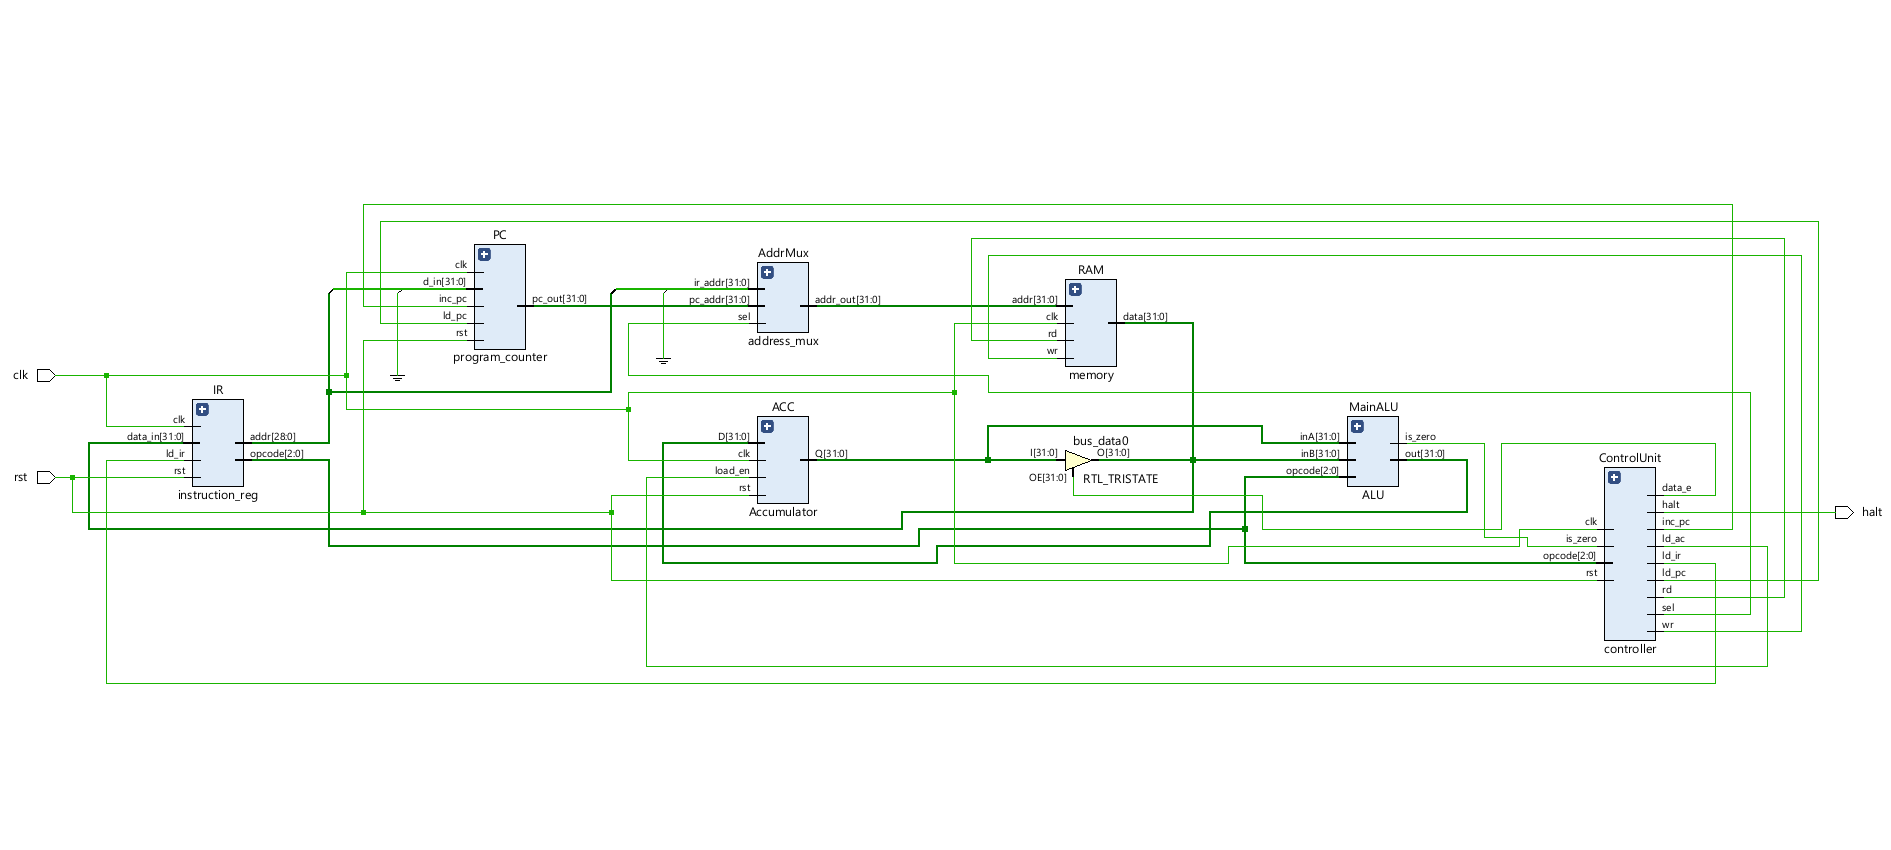
\includegraphics[width=0.9\textwidth]{sodocpu.png} 
    \caption{Sơ đồ mạch tích hợp hệ thống CPU (RTL Schematic)}
    \label{fig:cpu_top_rtl}
\end{figure}
    \newpage

    \section{KIỂM THỬ VÀ ĐÁNH GIÁ}

% 5.1. Testbench từng module
\subsection{Testbench từng module}
%\subsubsection{Testbench và Kết quả mô phỏng Program Counter (PC)}

\textbf{a. Mô tả kịch bản kiểm chứng (Testbench)} \\
Môi trường mô phỏng khối Program Counter được thiết lập nhằm xác minh khả năng quản lý luồng địa chỉ lệnh của CPU. Các kịch bản kiểm thử tập trung vào tính đúng đắn của logic điều khiển và cơ chế ưu tiên tín hiệu:
\begin{itemize}
    \item \textbf{Kiểm tra Reset đồng bộ}: Xác minh \texttt{pc\_out} quay về 0 ngay khi có sườn dương clock tác động trong lúc \texttt{rst} ở mức cao.
    \item \textbf{Kiểm tra tăng địa chỉ (\texttt{inc\_pc})}: Mô phỏng giai đoạn Fetch thông thường, mỗi chu kỳ địa chỉ tăng thêm 1 đơn vị.
    \item \textbf{Kiểm tra nạp địa chỉ (\texttt{ld\_pc})}: Mô phỏng lệnh nhảy (JMP), địa chỉ được nạp trực tiếp từ giá trị toán hạng \texttt{d\_in}.
    \item \textbf{Kiểm tra mức độ ưu tiên}: Kích hoạt đồng thời \texttt{ld\_pc} và \texttt{inc\_pc} để chứng minh hệ thống luôn ưu tiên nạp địa chỉ nhảy trước khi thực hiện tăng tuần tự.
\end{itemize}

\textbf{b. Mã nguồn Testbench (Verilog)}
\begin{lstlisting}[language=Verilog, caption={Ma nguon Testbench kiem tra Program Counter}]
`timescale 1ns / 1ps

module tb_program_counter();

    reg          clk;
    reg          rst;
    reg          ld_pc;
    reg          inc_pc;
    reg  [31:0]  d_in;
    wire [31:0]  pc_out;

    // Khoi tao module PC (Unit Under Test)
    program_counter uut (
        .clk(clk),
        .rst(rst),
        .ld_pc(ld_pc),
        .inc_pc(inc_pc),
        .d_in(d_in),
        .pc_out(pc_out)
    );

    // Tao xung clock chu ky 10ns
    always #5 clk = ~clk;

    initial begin
        // Khoi tao gia tri ban dau
        clk = 0; rst = 0; ld_pc = 0; inc_pc = 0; d_in = 32'b0;

        $display("-------");
        $display("Time|rst|ld_pc|inc_pc|d_in|pc_out");
        $display("-------");
        $monitor("%10t|%b|%b|%b|%h|%h", 
                 $time, rst, ld_pc, inc_pc, d_in, pc_out);

        // 1. Kiem tra Reset
        #12; rst = 1;
        #10; rst = 0;

        // 2. Kiem tra tang dia chi (inc_pc)
        #10; inc_pc = 1; // Tang len 1
        #10; inc_pc = 1; // Tang len 2
        #10; inc_pc = 0; // Dung tang, giu gia tri 2

        // 3. Kiem tra nap dia chi nhay (ld_pc)
        #10; d_in = 32'h0000_0ABC; ld_pc = 1;
        #10; ld_pc = 0; // Giu gia tri 0ABC

        // 4. Tang tu dia chi moi
        #10; inc_pc = 1;
        #10; inc_pc = 0; 

        // 5. Kiem tra uu tien: Vua nap vua tang (ld_pc phai thang)
        #10; d_in = 32'h0000_FFFF; ld_pc = 1; inc_pc = 1;
        #10; ld_pc = 0; inc_pc = 0; 

        #20;
        $display("-------");
        $display("Hoan thanh mo phong Program Counter!");
        $finish;
    end
endmodule
\end{lstlisting}

\textbf{c. Kết quả xuất ra màn hình (Console Output)} \\
Kết quả Console xác nhận PC luôn cập nhật giá trị khớp với các sự kiện điều khiển theo đúng kịch bản mô phỏng.

\begin{figure}[H]
    \centering
    % Thay 'pc_console.png' bang file anh console cua ban
    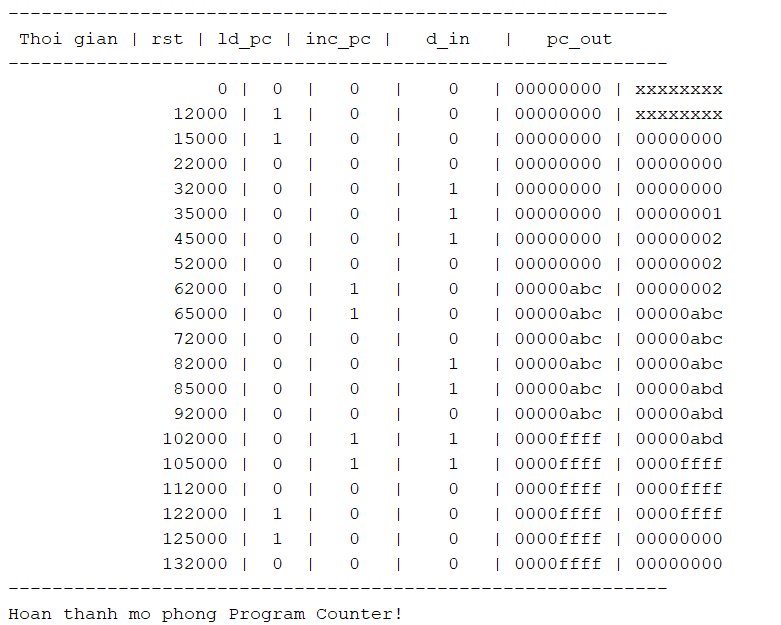
\includegraphics[width=0.8\textwidth]{consolepc.png} 
    \caption{Kết quả chạy Testbench Program Counter trên Console}
    \label{fig:pc_console}
\end{figure}

Dựa trên kết quả \texttt{\$monitor}, tại thời điểm $t=102ns$, khi cả hai tín hiệu \texttt{ld\_pc} và \texttt{inc\_pc} đều ở mức cao, ngõ ra \texttt{pc\_out} đã cập nhật giá trị từ \texttt{d\_in} (0xFFFF). Điều này minh chứng cấu trúc \texttt{if-else} trong module đã thực thi đúng mức ưu tiên thiết kế.

\textbf{d. Giản đồ sóng (Waveform)} \\
Sự thay đổi của bộ đếm PC được thể hiện rõ nét qua giản đồ thời gian, đảm bảo tính đồng bộ hoàn toàn với hệ thống.

\begin{figure}[H]
    \centering
    % Thay 'pc_waveform.png' bang file anh waveform cua ban
    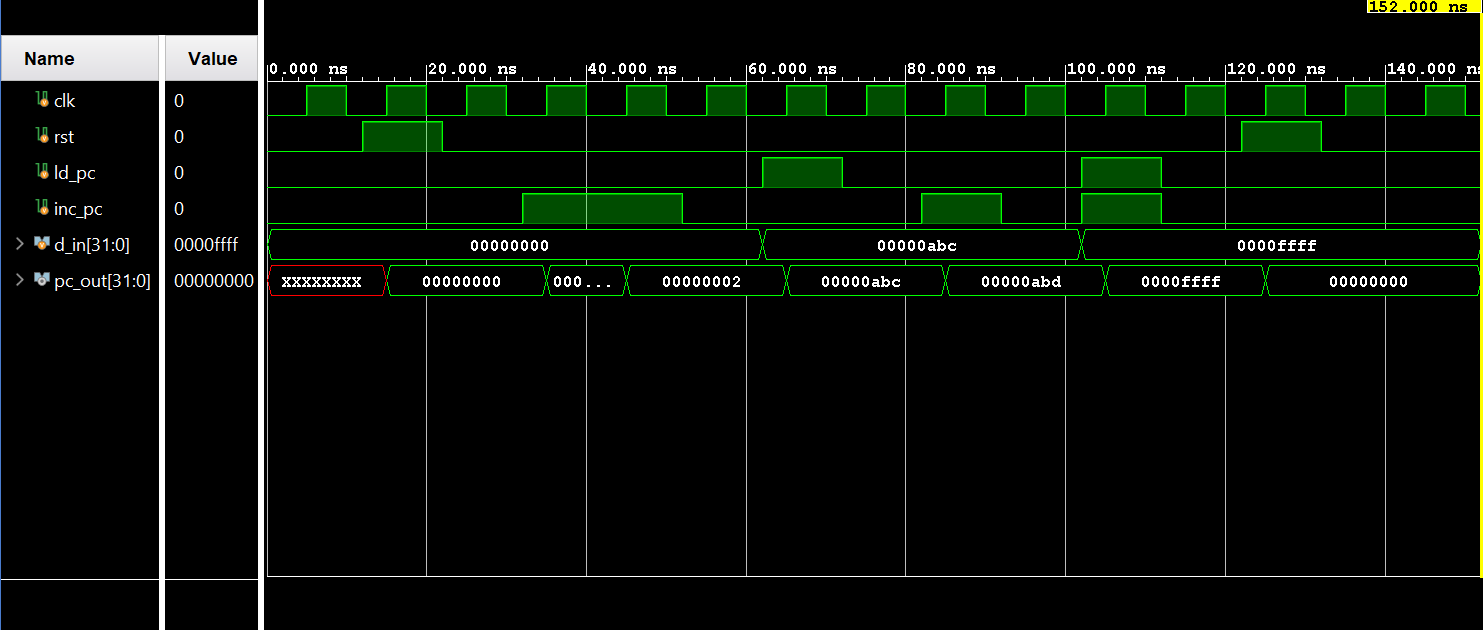
\includegraphics[width=\textwidth]{wavepc.png} 
    \caption{Giản đồ thời gian (Waveform) mô phỏng khối Program Counter}
    \label{fig:pc_waveform}
\end{figure}

Quan sát các sườn dương của xung clock (\texttt{clk}), địa chỉ \texttt{pc\_out} chỉ thay đổi trạng thái khi có sự tác động của \texttt{rst}, \texttt{ld\_pc} hoặc \texttt{inc\_pc}. Các khoảng thời gian còn lại, dữ liệu được duy trì ổn định, giúp việc truy xuất bộ nhớ lệnh không bị sai sót do nhiễu tín hiệu.
\textbf{e. Sơ đồ mạch RTL (RTL Schematic)} \\
Sơ đồ RTL sau khi tổng hợp cho thấy PC được hiện thực bằng các Flip-Flop 32-bit có tích hợp các bộ Mux điều khiển ở ngõ vào để chọn giữa các chế độ: Reset về 0, nạp dữ liệu nhảy hoặc tăng địa chỉ qua bộ cộng (Add Unit).

\begin{figure}[H]
    \centering
    % Nhớ chụp ảnh sơ đồ mạch trong Vivado và đặt tên file là 'pc_rtl.png'
    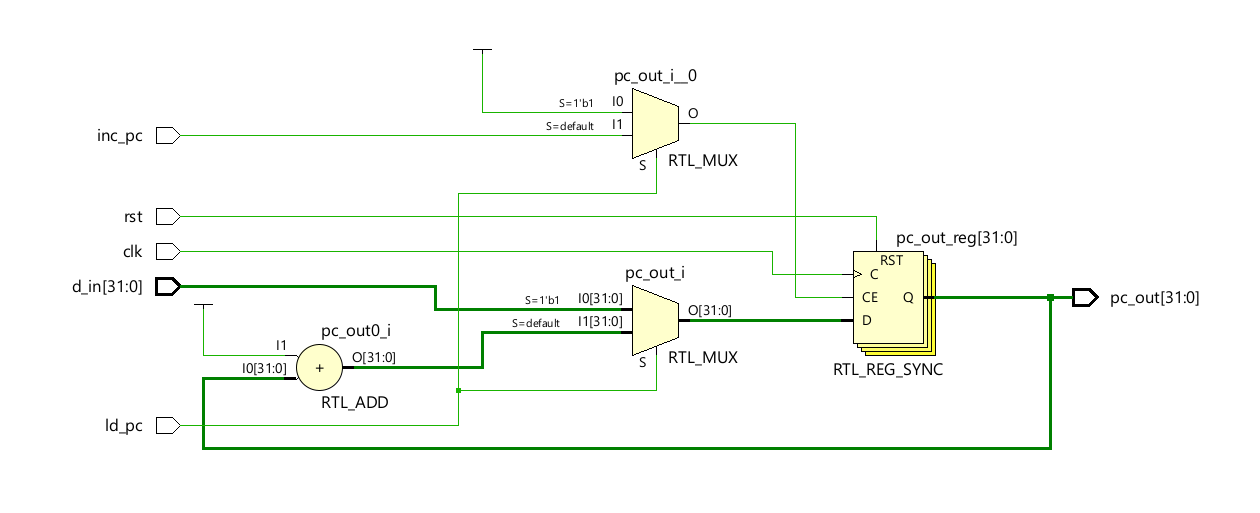
\includegraphics[width=\textwidth]{sodopc.png} 
    \caption{Sơ đồ mạch logic (RTL Schematic) của khối Program Counter}
    \label{fig:pc_rtl}
\end{figure}
%\subsubsection{Testbench và Kết quả mô phỏng Address Mux}

\textbf{a. Mô tả Testbench} \\
\begin{itemize}
    \item \textbf{Kiểm tra tính phản hồi tức thời}: Xác nhận ngõ ra \texttt{addr\_out} cập nhật ngay khi tín hiệu chọn \texttt{sel} 
    thay đổi mà không phụ thuộc vào xung clk.
    \item \textbf{Mô phỏng chu kỳ máy}: 
        \begin{itemize}
            \item Thiết lập \texttt{sel = 1} để kiểm tra luồng địa chỉ từ Program Counter (giai đoạn Fetch).
            \item Thiết lập \texttt{sel = 0} để kiểm tra luồng địa chỉ từ Instruction Register (giai đoạn Execute).
        \end{itemize}
    \item \textbf{Kiểm tra tính độc lập}: Thay đổi dữ liệu tại ngõ vào không được chọn 
    để đảm bảo ngõ ra vẫn giữ nguyên giá trị từ nguồn đã chọn.
\end{itemize}

\textbf{b. Mã nguồn Testbench}
\begin{lstlisting}[language=Verilog, caption={Ma nguon Testbench kiem tra Address Mux}]
`timescale 1ns / 1ps

module tb_address_mux();

    // Khai bao tham so do rong bit
    parameter W = 32;

    reg  [W-1:0] pc_addr;
    reg  [W-1:0] ir_addr;
    reg          sel;
    wire [W-1:0] addr_out;

    // Khoi tao module Address Mux voi tham so W 
    address_mux #(.WIDTH(W)) uut (
        .pc_addr(pc_addr),
        .ir_addr(ir_addr),
        .sel(sel),
        .addr_out(addr_out)
    );

    initial begin
        $display("-----------");
        $display(" Time|sel|pc_addr|ir_addr|addr_out");
        $display("-----------");
        $monitor("%10t|%b|%h|%h|%h", 
                 $time, sel, pc_addr, ir_addr, addr_out);

        // Khoi tao gia tri ban dau
        pc_addr = 32'h0000_1000; // Dia chi lenh 
        ir_addr = 32'h0000_ABCD; // Dia chi toan hang 
        sel = 0;

        //Test chon ir_addr 
        #10; sel = 0; 
        //Test chon pc_addr 
        #10; sel = 1;

        //Thay doi pc_addr khi dang chon pc_addr
        #10; pc_addr = 32'h0000_1004;

        //Thay doi ir_addr khi dang chon pc_addr (addr_out khong doi)
        #10; ir_addr = 32'h0000_EEEE;

        //Chuyen sang chon ir_addr
        #10; sel = 0;

        #10;
        $display("-----------");
        $display("Hoan thanh mo phong Address Mux!");
        $finish;
    end
endmodule
\end{lstlisting}

\textbf{c. Sơ đồ mạch RTL} \\
Sơ đồ RTL xác nhận khối được tổng hợp thành một bộ dồn kênh 2-sang-1 đơn giản, với đường dẫn dữ liệu từ hai nguồn đầu vào hội tụ tại một bộ chọn được điều khiển bởi tín hiệu \texttt{sel}.

\begin{figure}[H]
    \centering
    % Thay 'mux_rtl.png' bang ten file anh cua ban
    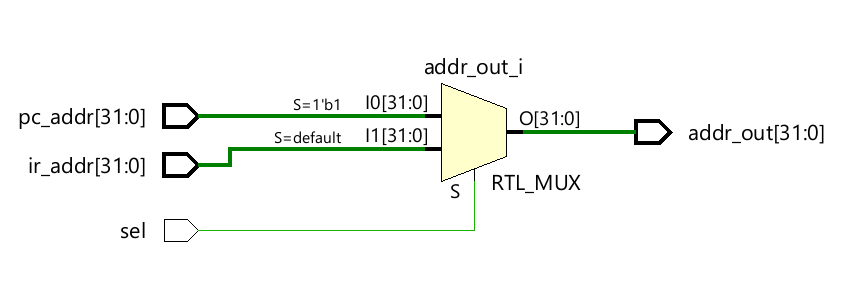
\includegraphics[width=0.6\textwidth]{sodoadd.png} 
    \caption{Sơ đồ mạch RTL của khối Address Mux}
    \label{fig:mux_rtl}
\end{figure}

\textbf{d. Kết quả xuất ra màn hình} \\
Kết quả Console minh chứng cho logic chuyển mạch tức thời của module.

\begin{figure}[H]
    \centering
    % Thay 'mux_console.png' bang ten file anh console cua ban
    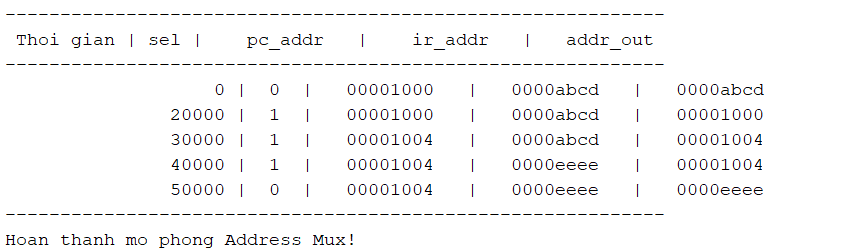
\includegraphics[width=0.8\textwidth]{consoleadd.png} 
    \caption{Kết quả chạy Testbench Address Mux trên Console}
    \label{fig:mux_console}
\end{figure}

Dựa trên bảng kết quả, tại thời điểm \texttt{sel = 1}, \texttt{addr\_out} luôn bám sát giá trị của \texttt{pc\_addr}. 
Khi thay đổi \texttt{ir\_addr} trong khi \texttt{sel} vẫn bằng 1, ngõ ra hoàn toàn không bị ảnh hưởng.

\textbf{e. Giản đồ sóng} \\

\begin{figure}[H]
    \centering
    % Thay 'mux_waveform.png' bang ten file anh waveform cua ban
    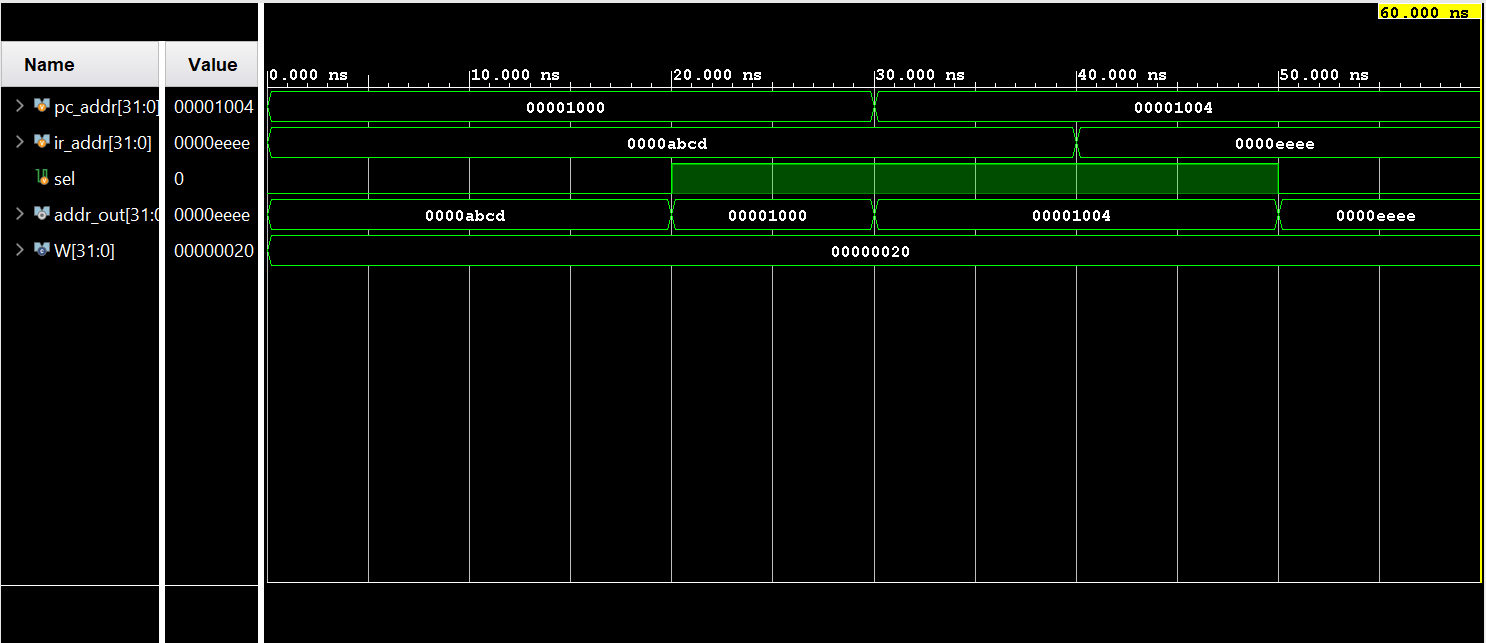
\includegraphics[width=\textwidth]{waveadd.png} 
    \caption{Giản đồ sóng mô phỏng khối Address Mux}
    \label{fig:mux_waveform}
\end{figure}

\subsubsection{Testbench và Kết quả mô phỏng ALU}

\textbf{a. Mô tả kịch bản kiểm chứng (Testbench)} \\
Môi trường mô phỏng (Testbench) được xây dựng nhằm kiểm tra toàn diện chức năng của khối số học và logic (ALU). Kịch bản kiểm tra (stimulus) được thiết kế với các mục tiêu cụ thể:
\begin{itemize}
    \item \textbf{Quét toàn bộ tập lệnh:} Lần lượt cấp các tín hiệu \texttt{opcode} từ \texttt{000} đến \texttt{111} kết hợp với các giá trị \texttt{inA} và \texttt{inB} khác nhau để kiểm tra ngõ ra \texttt{out}.
    \item \textbf{Kiểm tra tính bất đồng bộ của \texttt{is\_zero}:} Thử nghiệm thay đổi \texttt{inA} đột ngột để quan sát sự phản hồi ngay lập tức của cờ \texttt{is\_zero} mà không cần phụ thuộc vào xung clock hay sự thay đổi của \texttt{opcode}.
    \item \textbf{Bẫy lỗi (Corner Case):} Tạo test case số 9 thực hiện phép cộng số bù 2: $10 + (-10)$. Kết quả phép tính bằng 0 nhưng toán hạng \texttt{inA} $\neq 0$. Mục tiêu là chứng minh cờ \texttt{is\_zero} chỉ phụ thuộc vào \texttt{inA} theo đúng đặc tả của lệnh nhảy \texttt{SKZ}.
\end{itemize}

\textbf{b. Mã nguồn Testbench (Verilog)}
\begin{lstlisting}[language=Verilog, caption={Mã nguồn Testbench kiểm tra khối ALU}, label={lst:tb_alu}]
`timescale 1ns / 1ps

module tb_ALU();

    
    reg  [31:0] inA;
    reg  [31:0] inB;
    reg  [2:0]  opcode;
    
    wire [31:0] out;
    wire        is_zero;

    
    localparam HLT = 3'b000, SKZ = 3'b001, ADD = 3'b010, AND = 3'b011,
               XOR = 3'b100, LDA = 3'b101, STO = 3'b110, JMP = 3'b111;

    
    ALU uut (
        .inA(inA),
        .inB(inB),
        .opcode(opcode),
        .out(out),
        .is_zero(is_zero)
    );

   
    initial begin
       
$display("--------");
        $display("Time|Opcode|inA(hex)|inB(hex)|out(hex)|is_zero");
        $display("-------");
        
       
        $monitor("%8t|%b|%h|%h|%h|%b", 
                 $time, opcode, inA, inB, out, is_zero);

        
        inA = 32'd0; 
        inB = 32'd0; 
        opcode = HLT;
        #10; 
        
        // TEST CASE 1:  ADD 
       
        inA = 32'd15; 
        inB = 32'd25; 
        opcode = ADD;
        #10; 

       
        // TEST CASE 2:  AND 
        
        inA = 32'hFFFF0000; 
        inB = 32'hFF00FF00; 
        opcode = AND;
        #10; 

        
        // TEST CASE 3: XOR
        
        inA = 32'hAAAAAAAA; 
        inB = 32'h55555555; 
        opcode = XOR;
        #10; 

       
        // TEST CASE 4:  LDA (Load inB)
       
        inA = 32'd99; 
        inB = 32'h1234ABCD; 
        opcode = LDA;
        #10; 

       
        // TEST CASE 5:  inA (HLT, SKZ, STO, JMP)
       
        inA = 32'hCAFEBA5E; 
        inB = 32'd0; 
        opcode = STO;
        #10; 

      
        // TEST CASE 6:  is_zero 
       
        inA = 32'd0; 
        inB = 32'd999; 
        opcode = ADD;
        #10; 

      
        // TEST CASE 7:  SKZ with inA = 0
      
        inA = 32'd0; 
        inB = 32'hFFFFFFFF; 
        opcode = SKZ;
        #10; 

        
        // TEST CASE 8: is_zero nhay su thay doi inA ko thay doi opcode
      
        inA = 32'd5;
        #5;  
        inA = 32'd0;
        #5;  
        
        
        // TEST CASE 9: inA != 0 but result=0
inA = 32'd10;
inB = -32'd10; 
opcode = ADD;
#10;


        $display("-----------");
        $display("HOAN THANH MO PHONG!");
        $finish; 
    end

endmodule

\end{lstlisting}

\textbf{c. Sơ đồ mạch RTL (RTL Schematic)} \\
Quá trình tổng hợp (Synthesis) từ mã nguồn Verilog đã tạo ra sơ đồ mạch logic của ALU. Sơ đồ cho thấy bộ dồn kênh (Multiplexer) được tối ưu hóa để định tuyến dữ liệu dựa trên tín hiệu \texttt{opcode}, và một bộ dò cờ Zero (Zero Flag Detector) được kết nối trực tiếp vào bus \texttt{inA}.

\begin{figure}[H]
    \centering
    % Hãy thay 'alu_rtl_schematic.png' bằng ảnh sơ đồ mạch ALU xuất ra từ phần mềm (Vivado/Quartus)
    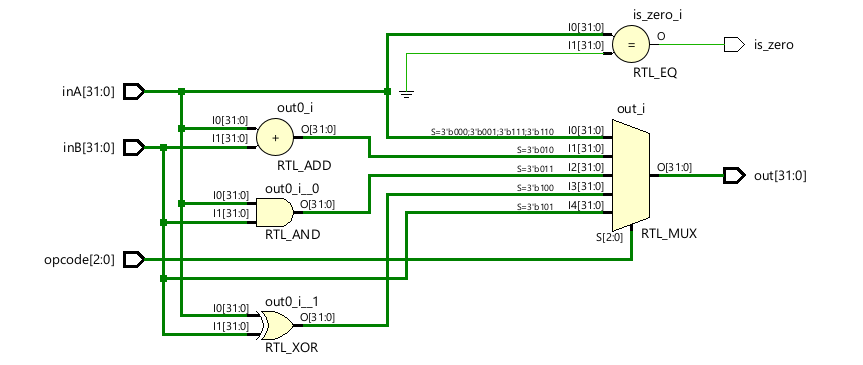
\includegraphics[width=0.85\textwidth]{machALU.png} 
    \caption{Sơ đồ mạch logic (RTL Schematic) của khối ALU}
    \label{fig:alu_rtl}
\end{figure}

\textbf{d. Kết quả xuất ra màn hình (Console Output)} \\
Thông qua các hàm hệ thống \texttt{\$monitor} và \texttt{\$display}, toàn bộ sự kiện thay đổi tín hiệu được ghi nhận lại theo thời gian thực.

\begin{figure}[H]
    \centering
    % Hãy thay 'alu_console.png' bằng ảnh chụp màn hình terminal Vivado của bạn
    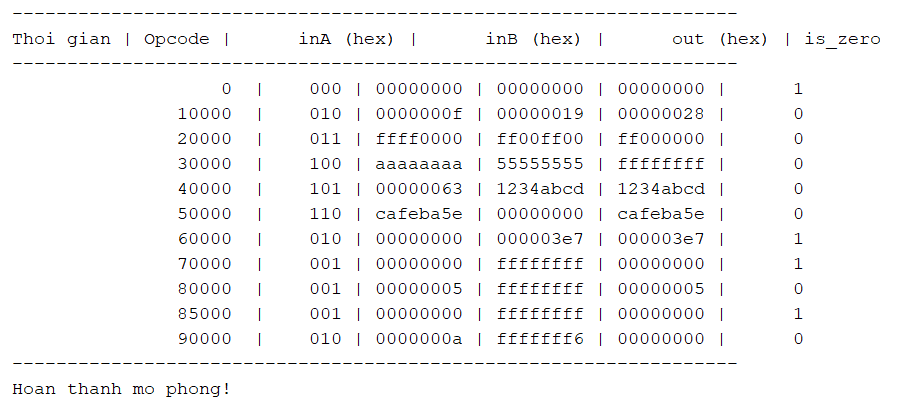
\includegraphics[width=0.75\textwidth]{cosoleALU.png} 
    \caption{Kết quả chạy Testbench khối ALU hiển thị trên Console}
    \label{fig:alu_console}
\end{figure}

Dựa vào bảng kết quả trên Console, các phép toán \texttt{ADD}, \texttt{AND}, \texttt{XOR} và các lệnh nạp dữ liệu hoạt động hoàn toàn chính xác. Tại thời điểm 90000 ps, phép toán \texttt{10 + (-10)} cho ra \texttt{out = 00000000} nhưng \texttt{is\_zero = 0} (vì \texttt{inA = 0000000a}), minh chứng thiết kế đã đúng tính chất bất đồng bộ .

\textbf{e. Giản đồ sóng (Waveform)} \\
Giản đồ thời gian cung cấp cái nhìn trực quan nhất về sự thay đổi của các tín hiệu điện. 

\begin{figure}[H]
    \centering
    % Hãy thay 'alu_waveform.png' bằng ảnh chụp giản đồ sóng của bạn
    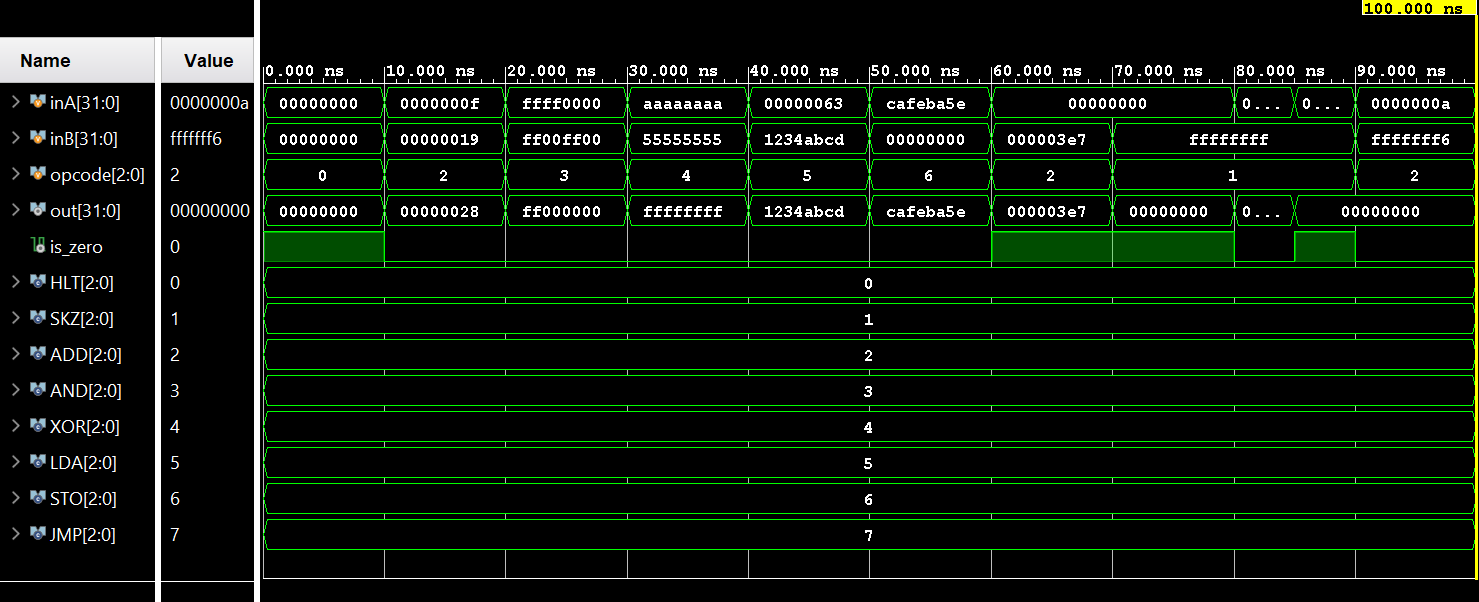
\includegraphics[width=\textwidth]{waveALU.png} 
    \caption{Giản đồ thời gian (Waveform) minh họa hoạt động của ALU}
    \label{fig:alu_waveform}
\end{figure}

Trên giản đồ sóng, có thể dễ dàng nhận thấy cờ \texttt{is\_zero} chuyển trạng thái ngay lập tức khi đường bus \texttt{inA} chuyển về mức 0. Đường \texttt{out} cũng phản hồi chính xác theo sự phối hợp của \texttt{inA}, \texttt{inB} và sự thay đổi của \texttt{opcode}.
%\subsubsection{Testbench và Kết quả mô phỏng Khối điều khiển (Controller)}

\textbf{a. Mô tả kịch bản kiểm chứng (Testbench)} \\
Môi trường mô phỏng khối Controller được thiết lập để kiểm tra chu trình 8 trạng thái (8-Phase) và sự chính xác của các tín hiệu điều khiển đầu ra ứng với từng loại mã lệnh (Opcode). Các kịch bản bao gồm:
\begin{itemize}
    \item \textbf{Khởi tạo và Fetch}: Kiểm tra 4 trạng thái đầu (\texttt{INST\_ADDR} đến \texttt{IDLE}) xem các tín hiệu \texttt{sel}, \texttt{rd}, \texttt{ld\_ir} có bật đúng để nạp lệnh hay không.
    \item \textbf{Lệnh tính toán (ADD/LDA)}: Kiểm tra việc bật tín hiệu \texttt{rd} ở giai đoạn thực thi và tín hiệu \texttt{ld\_ac} ở trạng thái \texttt{STORE}.
    \item \textbf{Lệnh rẽ nhánh (SKZ)}: Kiểm tra tín hiệu \texttt{inc\_pc} có bật thêm ở trạng thái \texttt{ALU\_OP} khi cờ \texttt{is\_zero = 1} hay không.
    \item \textbf{Lệnh nhảy (JMP)}: Kiểm tra tín hiệu \texttt{ld\_pc} có kích hoạt tại trạng thái thực thi để nạp địa chỉ mới.
    \item \textbf{Lệnh lưu trữ (STO)}: Kiểm tra sự phối hợp giữa \texttt{data\_e} và \texttt{wr} để ghi dữ liệu ra bộ nhớ.
\end{itemize}

\textbf{b. Mã nguồn Testbench (Verilog)}
\begin{lstlisting}[language=Verilog, caption={Ma nguon Testbench kiem tra khoi Controller}]
`timescale 1ns / 1ps

module tb_controller();
    // Khai bao cac tin hieu ket noi voi Module Controller
    reg clk;
    reg rst;
    reg [2:0] opcode;
    reg is_zero;
    
    wire sel, rd, ld_ir, halt, inc_pc, ld_ac, ld_pc, wr, data_e;
    wire [2:0] debug_state;

    // Khoi tao Unit Under Test (UUT)
    controller uut (
        .clk(clk), 
        .rst(rst), 
        .opcode(opcode), 
        .is_zero(is_zero),
        .sel(sel), 
        .rd(rd), 
        .ld_ir(ld_ir), 
        .halt(halt), 
        .inc_pc(inc_pc), 
        .ld_ac(ld_ac), 
        .ld_pc(ld_pc), 
        .wr(wr), 
        .data_e(data_e), 
        .debug_state(debug_state)
    );

    // Dinh nghia Opcode giong nhu trong module Controller
    localparam HLT=3'b000, SKZ=3'b001, ADD=3'b010, STO=3'b110, JMP=3'b111;

    // Tao xung clock chu ky 10ns
    always #5 clk = ~clk;

    initial begin
        // --- BUOC 0: Khoi tao he thong ---
        clk = 0; rst = 1; is_zero = 0; opcode = HLT;
        #15 rst = 0; // Tha reset sau 1.5 chu ky clock

        // --- BUOC 1: Kiem tra lenh ADD (Tinh toan) ---
        // Ky vong: ld_ac phai bat o buoc STORE (State 7)
        opcode = ADD; 
        $display("Time=%0t | Bat dau lenh ADD", $time);
        repeat (8) @(posedge clk); 

        // --- BUOC 2: Kiem tra lenh SKZ khi ket qua truoc do bang 0 ---
        // Ky vong: inc_pc phai bat 2 lan (State 6 va State 7)
        opcode = SKZ; is_zero = 1;
        $display("Time=%0t | Bat dau lenh SKZ (Zero=1)", $time);
        repeat (8) @(posedge clk);

        // --- BUOC 3: Kiem tra lenh STO (Ghi bo nho) ---
        // Ky vong: wr va data_e phai bat o buoc STORE (State 7)
        opcode = STO; is_zero = 0;
        $display("Time=%0t | Bat dau lenh STO", $time);
        repeat (8) @(posedge clk);

        // --- BUOC 4: Kiem tra lenh JMP (Nhay dia chi) ---
        // Ky vong: ld_pc phai bat o State 6 va 7
        opcode = JMP;
        $display("Time=%0t | Bat dau lenh JMP", $time);
        repeat (8) @(posedge clk);

        // --- BUOC 5: Kiem tra lenh HLT (Dung he thong) ---
        opcode = HLT;
        $display("Time=%0t | Bat dau lenh HLT", $time);
        repeat (8) @(posedge clk);

        #50;
        $display("Mo phong ket thuc thanh cong!");
        $finish;
    end

    // Tu dong in ket qua ra Console de kiem tra nhanh
    initial begin
        $monitor("T=%4t | State=%d | Op=%b | Halt=%b | IncPC=%b | LdAC=%b | Wr=%b",
        $time, debug_state, opcode, halt, inc_pc, ld_ac, wr);
    end

endmodule
\end{lstlisting}

\textbf{c. Sơ đồ mạch RTL (RTL Schematic)} \\
Sơ đồ tổng hợp khối Controller thể hiện cấu trúc của một máy trạng thái hữu hạn bao gồm bộ đếm trạng thái, bộ giải mã trạng thái kế tiếp và khối logic tổ hợp để tạo ra các tín hiệu điều khiển dựa trên mã lệnh đầu vào.

\begin{figure}[H]
    \centering
    % Thay 'controller_rtl.png' bang ten file anh thuc te cua ban
    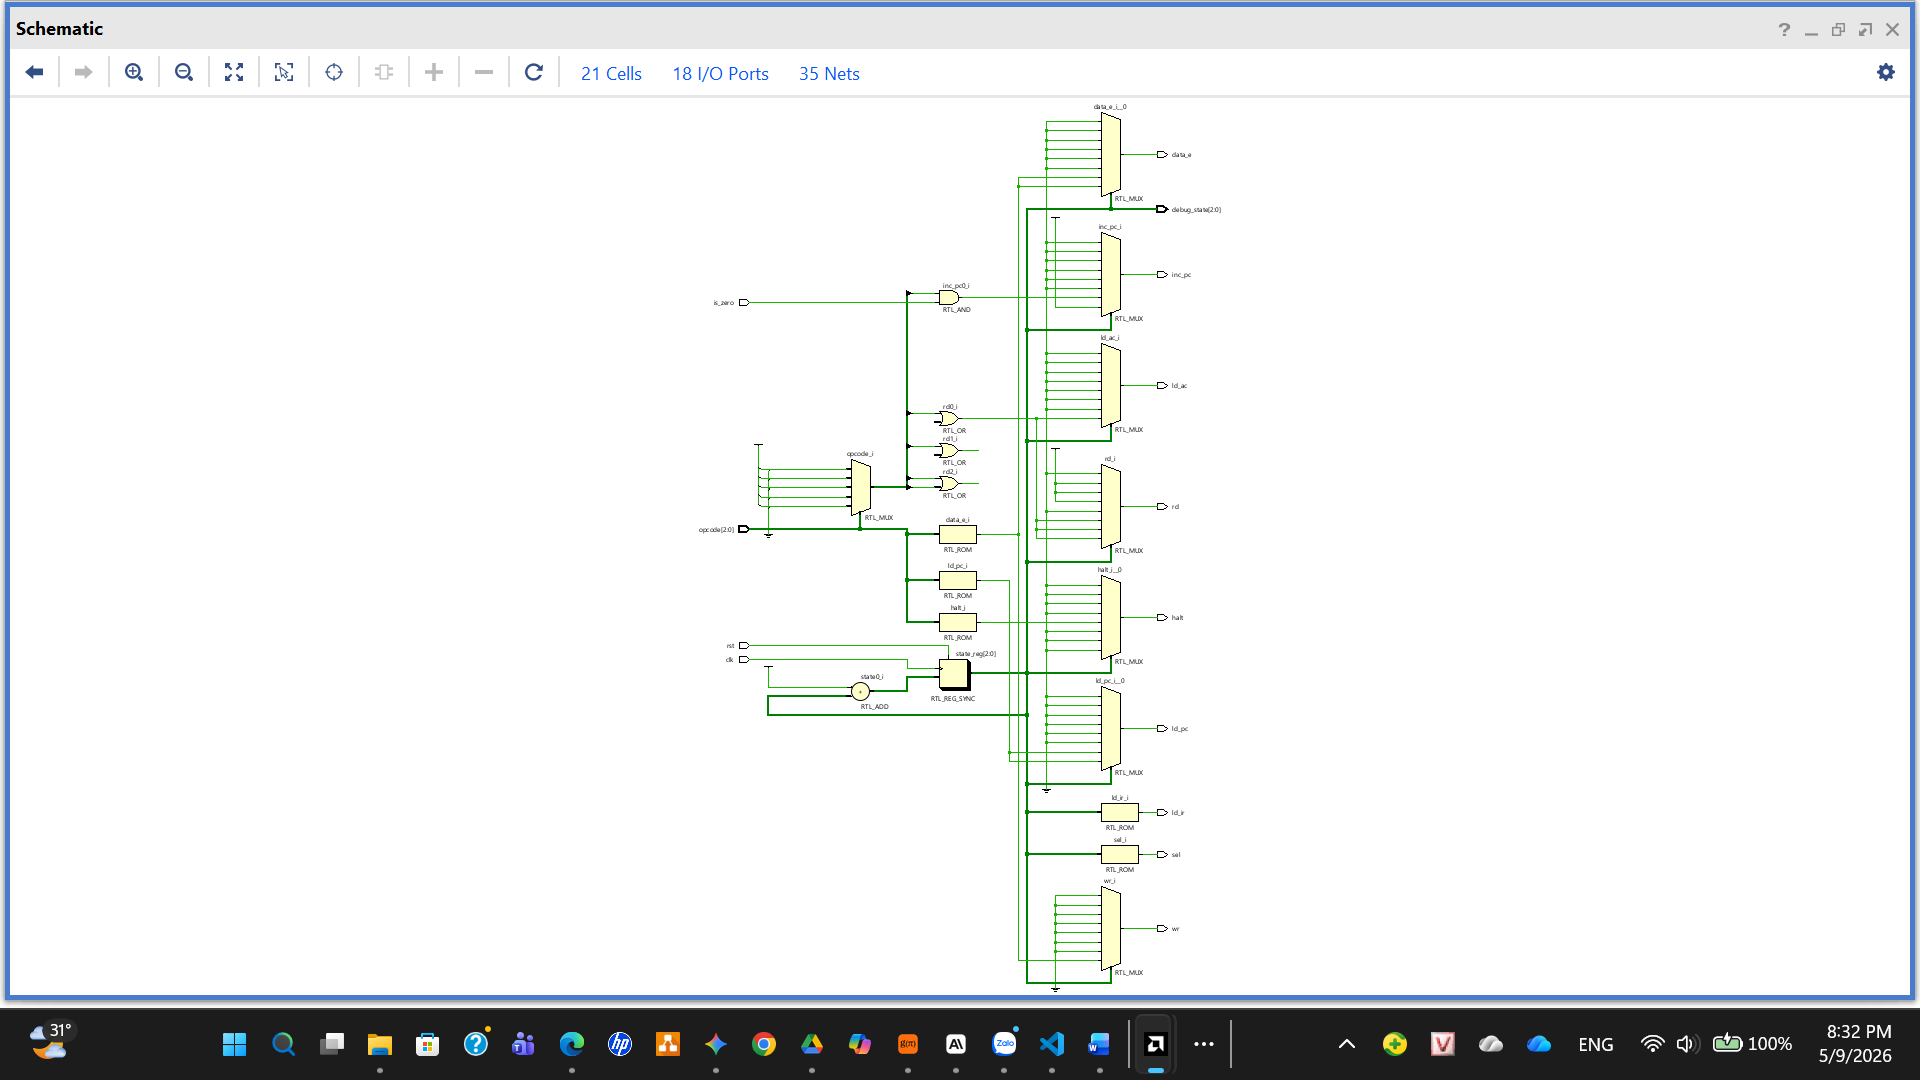
\includegraphics[width=0.9\textwidth]{sodocontrol.png} 
    \caption{Sơ đồ mạch logic (RTL Schematic) của khối Controller}
    \label{fig:ctrl_rtl}
\end{figure}

\textbf{d. Kết quả mô phỏng (Waveform)} \\
Quá trình chuyển đổi trạng thái và phản hồi của các tín hiệu điều khiển được ghi lại chi tiết trên giản đồ thời gian.

\begin{figure}[H]
    \centering
    % Thay 'controller_waveform.png' bang ten file anh thuc te cua ban
    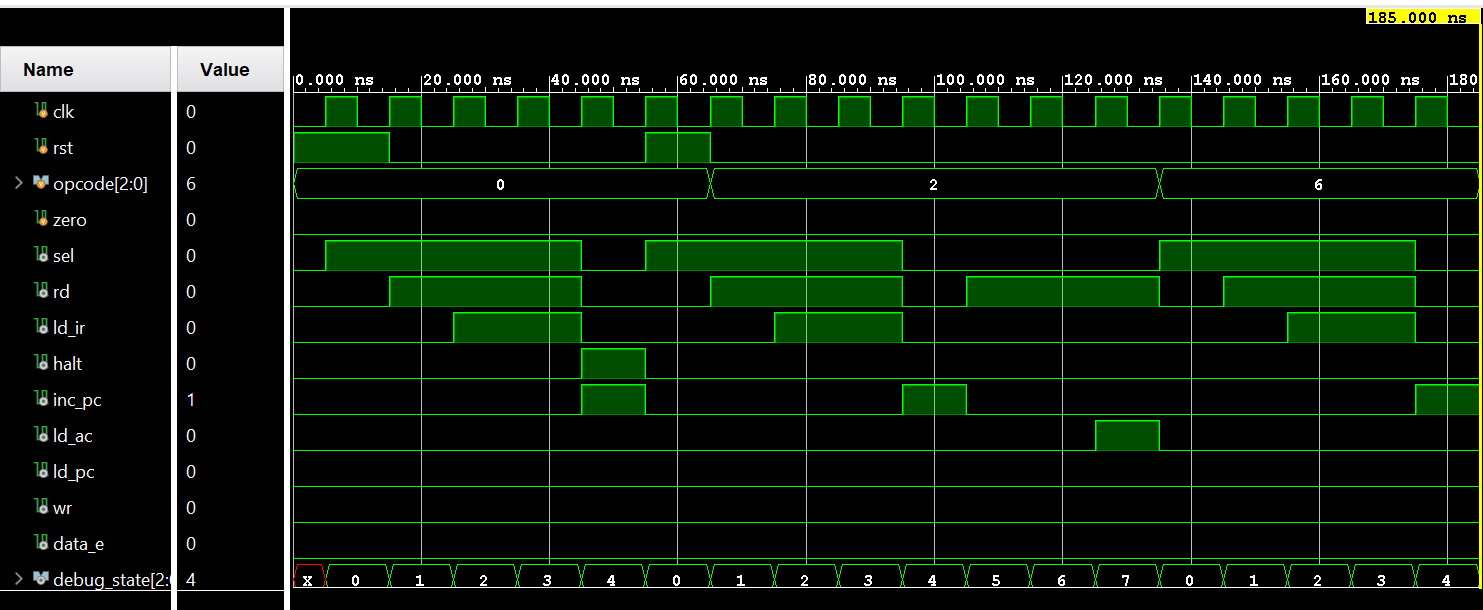
\includegraphics[width=\textwidth]{wavecontroller.png} 
    \caption{Giản đồ thời gian (Waveform) mô phỏng khối Controller}
    \label{fig:ctrl_wave}
\end{figure}

\textbf{e. Kết quả xuất ra màn hình (Console Output)} 
\begin{figure}[H]
    \centering
    % Thay 'controller_console.png' bang ten file anh thuc te cua ban
    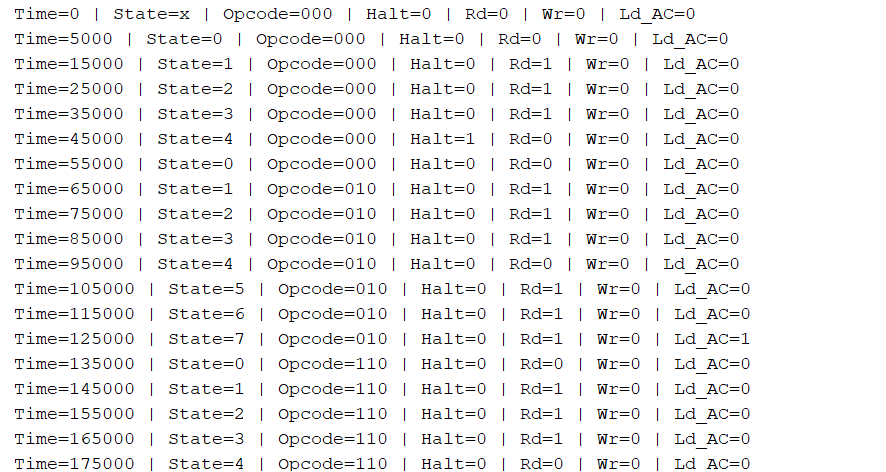
\includegraphics[width=0.8\textwidth]{1.png} 
    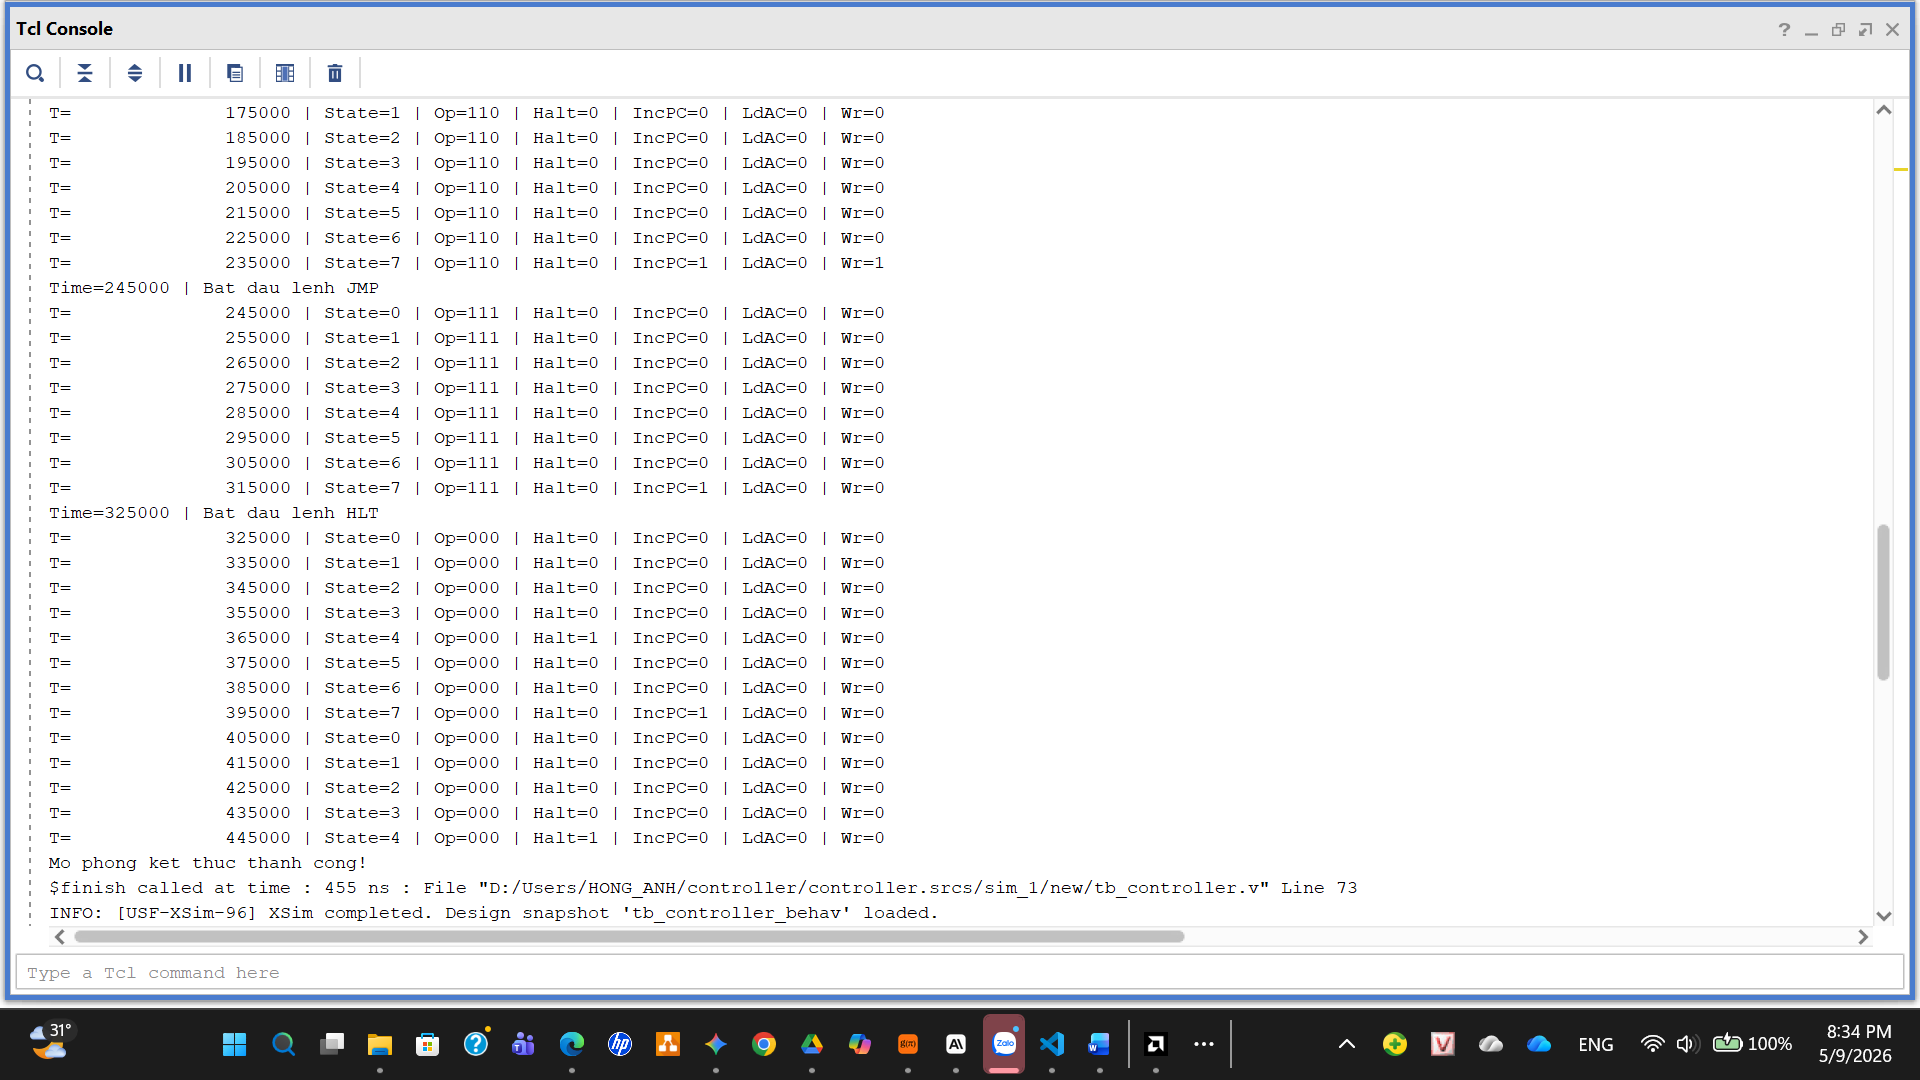
\includegraphics[width=0.8\textwidth]{2.png} 
    \caption{Kết quả Console mô phỏng khối Controller}
    \label{fig:ctrl_console}
\end{figure}

\textbf{Đánh giá kết quả:}
\begin{itemize}
    \item \textbf{Tính tuần tự}: Tín hiệu \texttt{debug\_state} thay đổi liên tục từ 0 đến 7, đảm bảo chu trình 8 bước không bị gián đoạn.
    \item \textbf{Đúng đắn về logic}: Tín hiệu \texttt{inc\_pc} luôn bật ở trạng thái \texttt{STORE} cho mọi lệnh, riêng với lệnh \texttt{SKZ} khi cờ \texttt{is\_zero = 1}, nó còn bật thêm ở trạng thái \texttt{ALU\_OP}, giúp nhảy qua lệnh kế tiếp chính xác như thiết kế.
    \item \textbf{Cơ chế nạp/ghi}: Tín hiệu \texttt{ld\_ac} (cho lệnh tính toán) và \texttt{wr} (cho lệnh ghi) chỉ xuất hiện ở bước cuối cùng, đảm bảo tính ổn định của dữ liệu trên Bus hệ thống trước khi thực hiện thao tác lưu trữ.
\end{itemize}
\input{phan5151.tex}
%\input{phan5152.tex}
%\subsubsection{Testbench và Kết quả mô phỏng Khối Bộ nhớ (Memory)}

\textbf{a. Mô tả kịch bản kiểm chứng (Testbench)} \\
Môi trường mô phỏng khối Memory được thiết lập để kiểm tra khả năng lưu trữ dữ liệu và tính đúng đắn của cổng giao tiếp song hướng (\textit{bidirectional port}). Các kịch bản kiểm thử bao gồm:
\begin{itemize}
    \item \textbf{Khởi tạo hệ thống}: Thiết lập các giá trị ban đầu và kiểm tra trạng thái trở kháng cao (\texttt{Hi-Z}) của bus dữ liệu khi không có lệnh đọc/ghi.
    \item \textbf{Thao tác Ghi (Write)}: Thực hiện ghi các giá trị dữ liệu cụ thể vào các địa chỉ khác nhau trong RAM tại cạnh lên của xung clock để kiểm tra tính đồng bộ.
    \item \textbf{Thao tác Đọc (Read)}: Truy xuất dữ liệu từ các địa chỉ đã ghi trước đó để đối chiếu tính toàn vẹn của dữ liệu.
    \item \textbf{Kiểm tra tách biệt Đọc/Ghi}: Đảm bảo rằng bus dữ liệu không bị xung đột khi chuyển đổi giữa chế độ đọc và ghi (sử dụng trạng thái trở kháng cao \texttt{32'bz}).
\end{itemize}

\textbf{b. Mã nguồn Testbench (Verilog)}
\begin{lstlisting}[language=Verilog, caption={Ma nguon Testbench kiem tra khoi Bo nho (Memory)}]
`timescale 1ns / 1ps

module tb_memory();

    reg          clk;
    reg  [31:0]  addr;
    reg          rd;
    reg          wr;
    wire [31:0]  data;

    reg  [31:0]  data_reg;
    assign data = (wr && !rd) ? data_reg : 32'bz;

    memory uut (
        .clk(clk),
        .addr(addr),
        .rd(rd),
        .wr(wr),
        .data(data)
    );

    always #5 clk = ~clk;

    initial begin
        clk = 0; addr = 0; rd = 0; wr = 0; data_reg = 0;

        $display("------------");
        $display(" Time|rd|wr|addr|data(hex)");
        $display("------------");
        
        // --- DONG QUAN TRONG NHAT: Monitor de in so lieu ra Console ---
        $monitor("%10t|%b|%b|%h|%h", $time, rd, wr, addr, data);

        // 1. Ghi du lieu vao o nho 0x01
        #10; addr = 32'h01; data_reg = 32'hABCD_1234; wr = 1; rd = 0;
        #10; wr = 0; 

        // 2. Ghi du lieu vao o nho 0x02
        #10; addr = 32'h02; data_reg = 32'h5555_AAAA; wr = 1;
        #10; wr = 0;

        // 3. Doc du lieu tu o nho 0x01
        #10; addr = 32'h01; rd = 1; wr = 0;
        #10; 
        
        // 4. Doc du lieu tu o nho 0x02
        #10; addr = 32'h02;
        #10;

        // 5. Trang thai nghi
        #10; rd = 0; wr = 0;
        #10;

        $display("------------");
        $display("Hoan thanh mo phong Memory!");
        $finish;
    end
endmodule
\end{lstlisting}

\textbf{c. Sơ đồ mạch RTL (RTL Schematic)} \\
Sơ đồ tổng hợp khối Memory thể hiện cấu trúc của mảng lưu trữ RAM và khối logic điều khiển cổng đệm ba trạng thái (\textit{Tri-state buffer}) phục vụ cho chân giao tiếp \texttt{inout}.

\begin{figure}[H]
    \centering
    % Thay 'sodomemory.png' bang ten file anh thuc te cua ban
    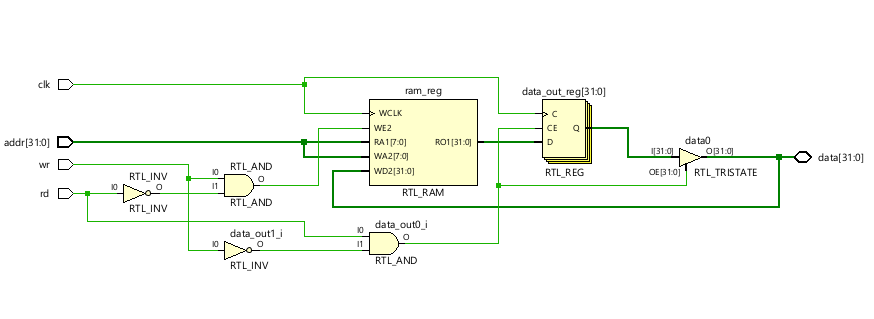
\includegraphics[width=0.8\textwidth]{sodomem.png} 
    \caption{Sơ đồ mạch logic (RTL Schematic) của khối Memory}
    \label{fig:mem_rtl}
\end{figure}

\textbf{d. Kết quả mô phỏng (Waveform)} \\
Sự thay đổi của bus dữ liệu khi thực hiện các thao tác ghi và đọc được thể hiện chi tiết trên giản đồ thời gian, đặc biệt là trạng thái trở kháng cao khi không có lệnh.

\begin{figure}[H]
    \centering
    % Thay 'wavememory.png' bang ten file anh thuc te cua ban
    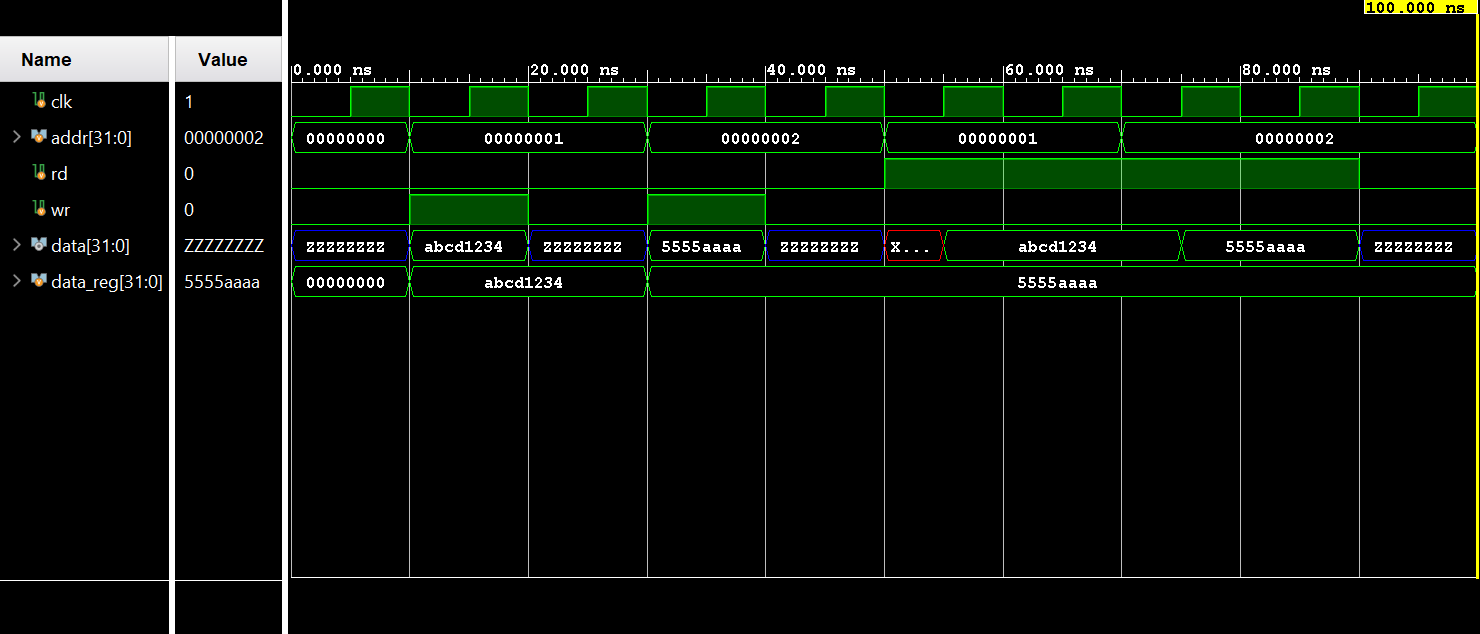
\includegraphics[width=\textwidth]{wavemem.png} 
    \caption{Giản đồ thời gian (Waveform) mô phỏng khối Memory}
    \label{fig:mem_wave}
\end{figure}

\textbf{e. Kết quả xuất ra màn hình (Console Output)} 
\begin{figure}[H]
    \centering
    % Thay 'console_memory.png' bang ten file anh thuc te cua ban
    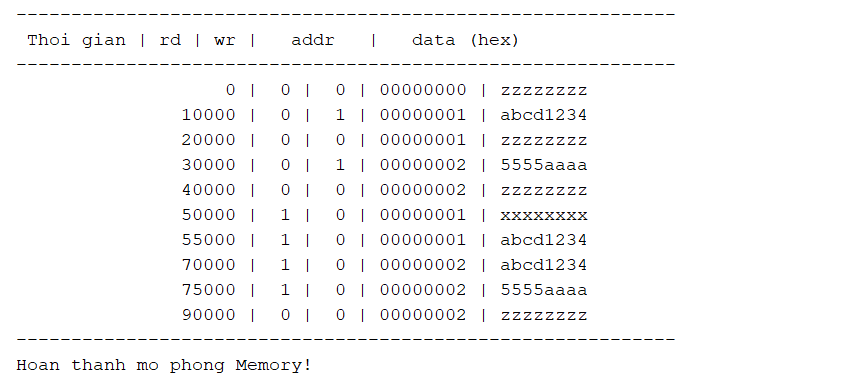
\includegraphics[width=0.8\textwidth]{consolemem.png} 
    \caption{Kết quả Console mô phỏng khối Memory}
    \label{fig:mem_console}
\end{figure}

\textbf{Đánh giá kết quả:}
\begin{itemize}
    \item \textbf{Cổng song hướng (Inout)}: Hoạt động chính xác theo cơ chế tri-state. Khi \texttt{rd=0} và \texttt{wr=0}, bus dữ liệu ở trạng thái \texttt{ZZZZZZZZ}, không gây xung đột trên đường truyền chung.
    \item \textbf{Tính đồng bộ}: Các thao tác ghi và đọc đều được kích hoạt tại cạnh lên của xung clock, đảm bảo dữ liệu được chốt vào ô nhớ và xuất ra bus ổn định, đúng nhịp hệ thống.
    \item \textbf{Độ tin cậy dữ liệu}: Kết quả đọc lại từ địa chỉ \texttt{0x01} (\texttt{ABCD\_1234}) và \texttt{0x02} (\texttt{5555\_AAAA}) hoàn toàn trùng khớp với dữ liệu đã ghi ban đầu, khẳng định mảng RAM và logic giải mã địa chỉ hoạt động đúng yêu cầu.
\end{itemize}

% 5.2. Kiểm thử tích hợp (Integration Test)
%\subsection{Kiểm thử tích hợp (Integration Test)}
%
\textbf{a. Mô tả Testbench} 
Chương trình kiểm thử thực hiện phép tính cộng hai số và lưu kết quả vào một địa chỉ đích trong bộ nhớ, gồm các bước:
\begin{itemize}
    \item \textbf{Khởi tạo}: Nạp mã máy của chương trình vào các địa chỉ đầu tiên của RAM.
    \item \textbf{Dữ liệu đầu vào}: Nạp giá trị \texttt{10} (tại địa chỉ \texttt{0x10}) và \texttt{20} (tại địa chỉ \texttt{0x11}).
    \item \textbf{Thực thi lệnh}: 
    \begin{itemize}
        \item \texttt{LDA 0x10}: Nạp giá trị 10 vào thanh ghi Accumulator.
        \item \texttt{ADD 0x11}: Cộng giá trị trong Accumulator với 20, kết quả tạm thời là 30.
        \item \texttt{STO 0x50}: Lưu kết quả (30) từ Accumulator vào địa chỉ bộ nhớ \texttt{0x50}.
        \item \texttt{HLT}: Dừng hệ thống.
    \end{itemize}
    \item \textbf{Kết quả dự tính}: Sau khi tín hiệu \texttt{halt} bật lên, giá trị tại ô nhớ \texttt{0x50} phải bằng \texttt{30}.
\end{itemize}

\textbf{b. Mã nguồn Testbench}

\begin{lstlisting}[language=Verilog, caption={Testbench CPU}]
`timescale 1ns / 1ps

module tb_CPU_System();
    reg clk, rst;
    wire halt;

    CPU_Top uut (.clk(clk), .rst(rst), .halt(halt));

    always #5 clk = ~clk;

    initial begin
        clk = 0; rst = 1;
        
        // Dia chi 0: LDA 0x10 (Opcode 101)
        uut.RAM.ram[0] = {3'b101, 29'h10}; 
        // Dia chi 1: ADD 0x11 (Opcode 010)
        uut.RAM.ram[1] = {3'b010, 29'h11};
        // Dia chi 2: STO 0x50 (Opcode 110)
        uut.RAM.ram[2] = {3'b110, 29'h50};
        // Dia chi 3: HLT (Opcode 000)
        uut.RAM.ram[3] = {3'b000, 29'h0};


        uut.RAM.ram[16] = 32'd10; // Tai dia chi 0x10
        uut.RAM.ram[17] = 32'd20; // Tai dia chi 0x11

        #15 rst = 0;

        wait(halt == 1);
        
        #20;
        $display("Ket qua tai dia chi 0x50: %d", uut.RAM.ram[80]);
        if (uut.RAM.ram[80] == 30) 
            $display("TEST SUCCESSFUL!");
        else 
            $display("TEST FAILED!");
            
        $finish;
    end
endmodule
\end{lstlisting}

\textbf{c. Kết quả xuất ra màn hình} 
\begin{figure}[H]
    \centering
    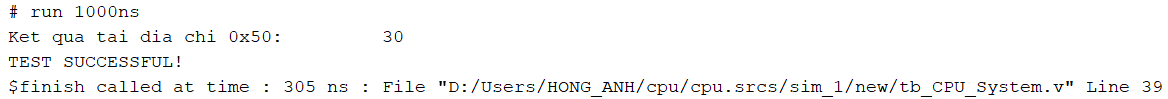
\includegraphics[width=0.8\textwidth]{consolecpu.png} 
    \caption{Kết quả Console thông báo trạng thái kiểm thử hệ thống}
    \label{fig:sys_console}
\end{figure}

\textbf{Đánh giá kết quả:}
\begin{itemize}
    \item \textbf{Luồng thực thi}: CPU thực hiện đúng quy trình Fetch-Decode-Execute cho từng lệnh. 
    Tín hiệu \texttt{halt} bật lên chính xác sau khi hoàn thành lệnh cuối cùng.
    \item \textbf{Độ chính xác dữ liệu}: Phép tính $10 + 20$ được ALU thực hiện chính xác.
    \item \textbf{Tương tác Memory}: Khối Memory đã đáp ứng tốt cả hai vai trò cung cấp mã lệnh và lưu trữ dữ liệu.
    \item \textbf{Kết luận}: Hệ thống tích hợp hoạt động ổn định.
\end{itemize}

\textbf{d. Giản đồ sóng} 

\begin{figure}[H]
    \centering
    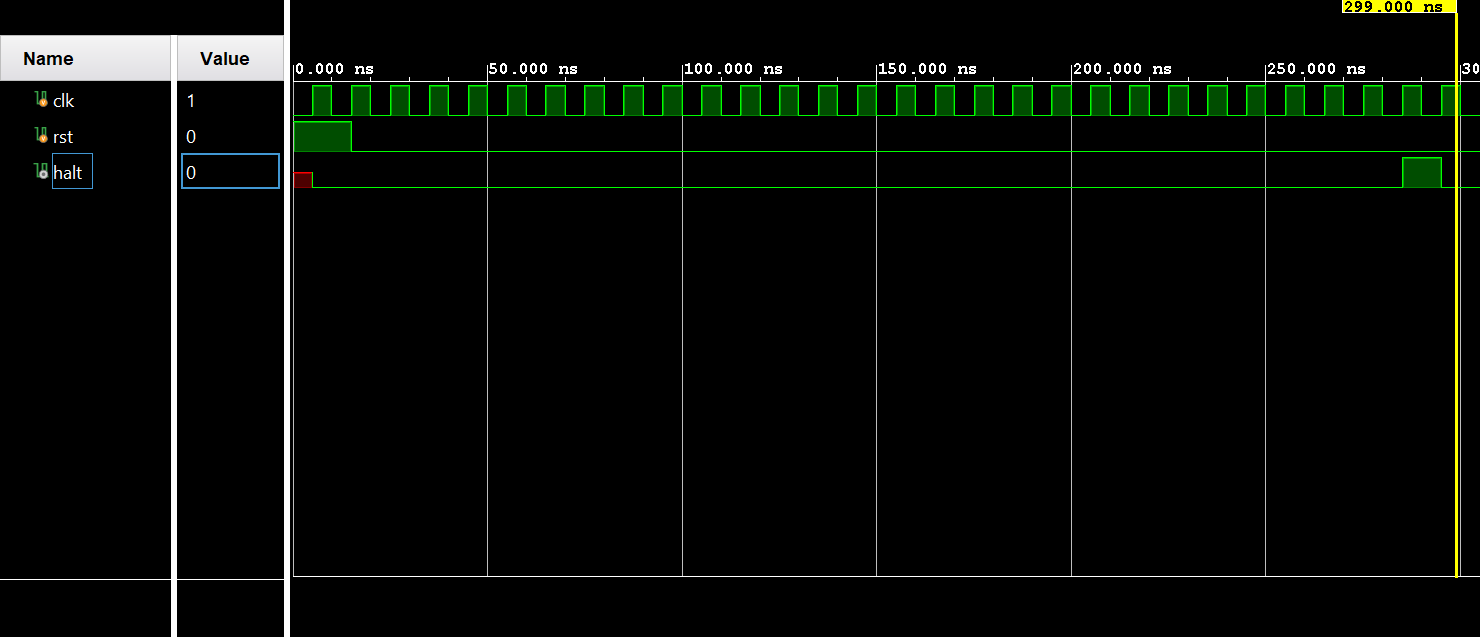
\includegraphics[width=\textwidth]{wavecpu.png} 
    \caption{Giản đồ sóng chương trình tính toán trên hệ thống CPU}
    \label{fig:sys_wave}
\end{figure}



% 5.3. Đánh giá hiệu năng
%\subsection{Đánh giá hiệu năng}
%
\subsection{Phân tích tài nguyên sử dụng}

Dựa trên kết quả từ bảng báo cáo, hệ thống sử dụng một lượng tài nguyên rất nhỏ so với tổng thể chip FPGA mục tiêu.

\begin{figure}[H]
    \centering
    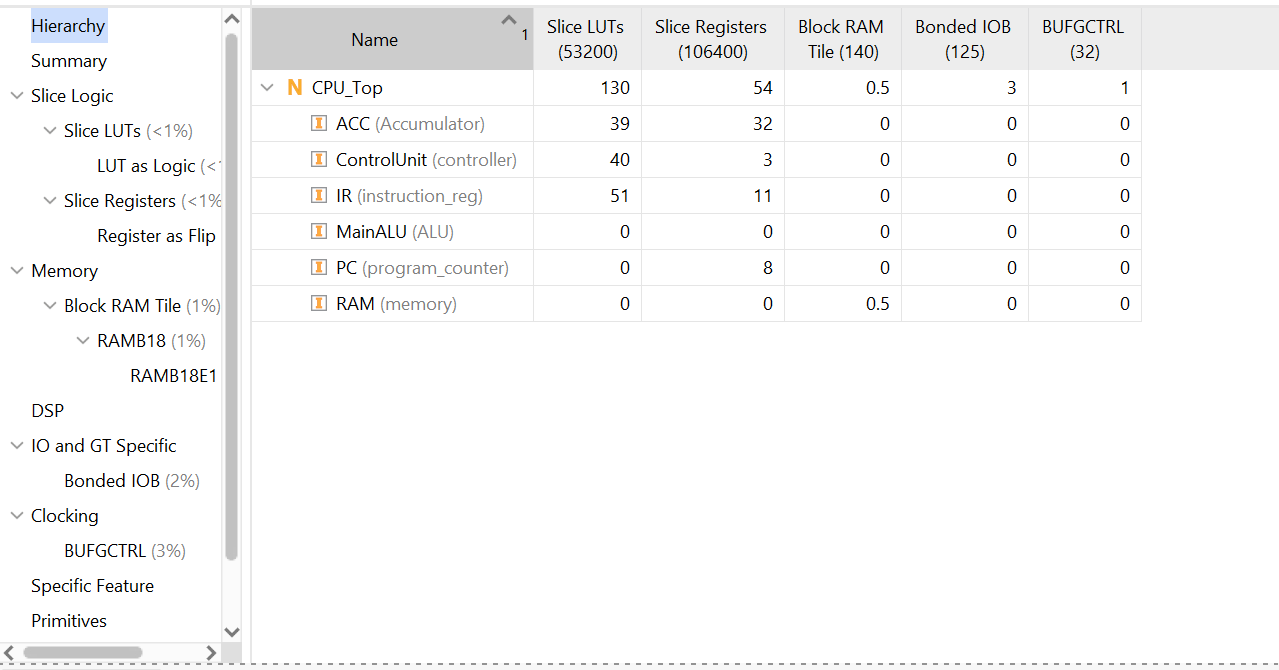
\includegraphics[width=0.9\textwidth]{ulti.png}
    \caption{Báo cáo tài nguyên Utilization chi tiết cho từng module}
    \label{fig:utilization}
\end{figure}


\subsection{Phân tích thời gian }

\begin{figure}[H]
    \centering
    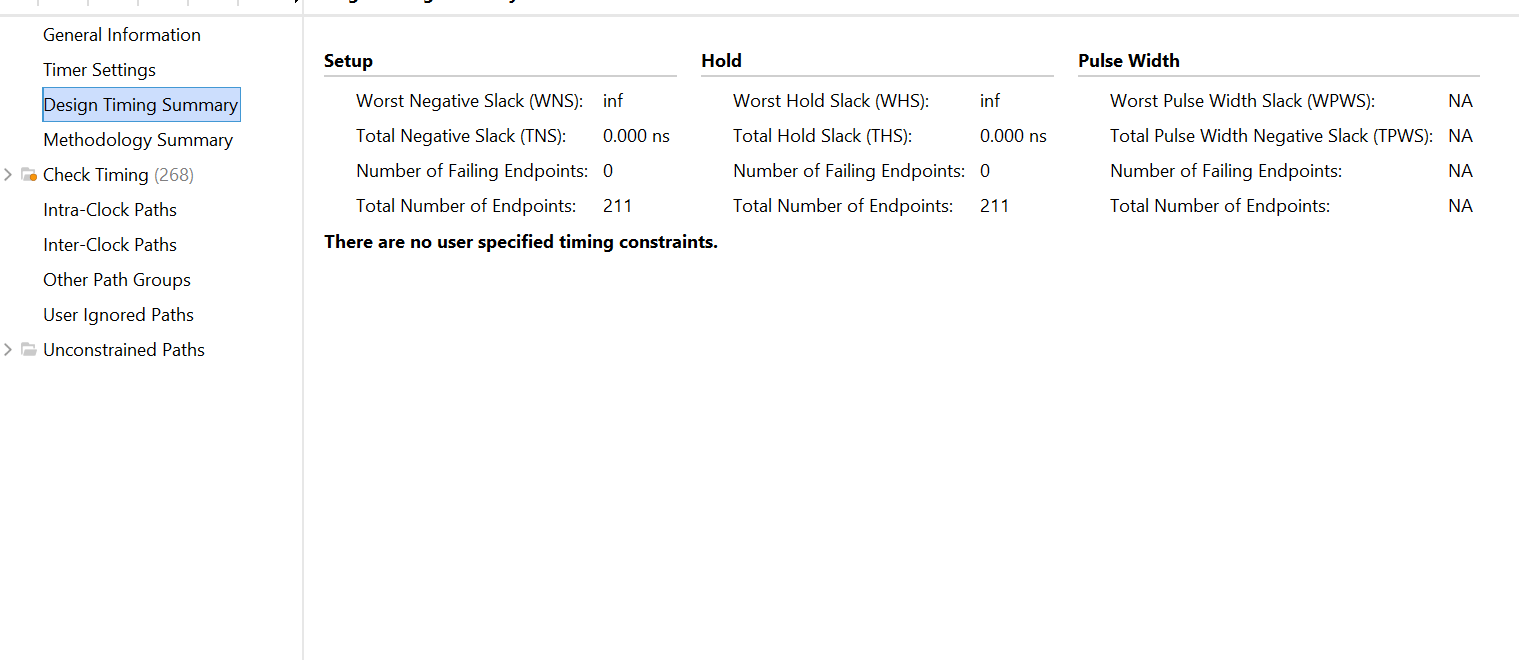
\includegraphics[width=0.9\textwidth]{time.png}
    \caption{Báo cáo phân tích thời gian Timing Summary}
    \label{fig:timing}
\end{figure}

\textbf{Nhận xét:}
\begin{itemize}
    \item \textbf{Độ tin cậy:} Chỉ số TNS (Total Negative Slack) bằng 0.000 ns và không có điểm lỗi cho thấy thiết kế ổn định.
    \item \textbf{Khả năng vận hành:} Mặc dù chưa thiết lập ràng buộc XDC cụ thể cho xung clock,
     nhưng với mật độ logic thấp hệ thống có thể đáp ứng tốt các ứng dụng yêu cầu tần số hoạt động 100MHz.
\end{itemize}

\subsection{Phân tích năng lượng tiêu thụ}

\begin{figure}[H]
    \centering
    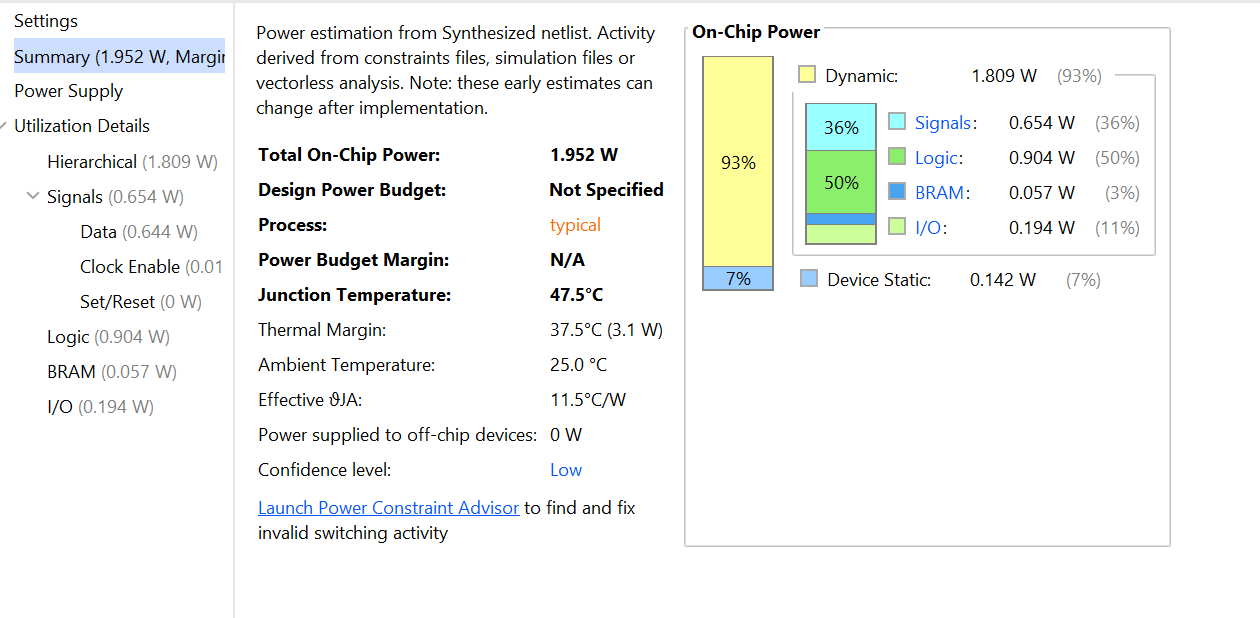
\includegraphics[width=0.8\textwidth]{power.png}
    \caption{Báo cáo ước tính năng lượng tiêu thụ và nhiệt độ hoạt động}
    \label{fig:power}
\end{figure}

\textbf{Nhận xét:}
\begin{itemize}
    \item \textbf{Hiệu suất năng lượng:} Tổng công suất tiêu thụ đạt 1.952 W. Trong đó, công suất động (Dynamic Power) chiếm tới 93\%, 
    cho thấy phần lớn năng lượng được tập trung cho các hoạt động đóng cắt cổng logic để xử lý lệnh.
    \item \textbf{Phân tích thành phần:} Logic chiếm 50\% và tín hiệu chiếm 36\% công suất động.
    \item \textbf{Độ ổn định nhiệt:} Nhiệt độ hoạt động duy trì ở mức 47.5°C. Đây là mức nhiệt lý tưởng để CPU có thể vận hành liên tục mà không bị quá nhiệt.
\end{itemize}
    \newpage

    \section{ KẾT LUẬN}


\subsection{Kết quả đạt được}
Thông qua quá trình nghiên cứu và thực hiện đồ án, nhóm đã đạt được các kết quả sau:
\begin{itemize}
    \item \textbf{Thiết kế hệ thống:} Hoàn thành việc thiết kế và mô phỏng một RISC CPU đơn giản dựa trên ngôn ngữ mô tả phần cứng Verilog. 
    \item \textbf{Kiến trúc phân khối:} Học tập các cấu trúc khối chức năng và khối điều khiển của một RISC CPU.
    \item \textbf{Năng lực chuyên môn:} Quen với việc sử dụng ngôn ngữ Verilog để đặc tả các sơ đồ khối, đồng thời học cách tạo các testbench một cách có chủ đích và qua đó
    nhóm còn học được cách viết một báo cáo gồm đầy đủ các nội dung.
\end{itemize}

\subsection{Khó khăn và Thách thức}
Trong quá trình triển khai, nhóm đã đối mặt và giải quyết các thách thức kỹ thuật sau:
\begin{itemize}
    \item \textbf{Bước đầu làm quen:} Choáng ngợp trước mô hình phức tạp, có quá nhiều khối chức năng và các đường truyền dễ lẫn lộn.
    \item \textbf{Làm việc nhóm: } Việc làm việc nhóm với một đề tài tương đối lớn gây nhiều khó khăn về mặt phân chia công việc và xác định deadline.
\end{itemize}

\subsection{Hướng phát triển và Mở rộng}
Nhằm nâng cao hiệu suất và tính ứng dụng của kiến trúc, nhóm đề xuất các hướng phát triển tiếp theo:
\begin{itemize}
    \item \textbf{Nâng cấp tập lệnh (ISA):} Mở rộng khả năng xử lý bằng cách tích hợp các phép toán phức tạp (nhân/chia), xử lý số dấu phẩy động và các chế độ địa chỉ gián tiếp.
    \item \textbf{Tối ưu hóa kiến trúc Pipeline:} Triển khai cấu trúc đường ống nhiều giai đoạn (IF, ID, EX, MEM, WB) nhằm tăng cường thông lượng (throughput) và khai thác tối đa tài nguyên phần cứng.
    \item \textbf{Triển khai phần cứng thực tế:} Thực hiện tổng hợp và nạp thiết kế lên bo mạch FPGA (như Arty Z7) để đánh giá các thông số về tài nguyên thực tế và tần số hoạt động tối đa. Đồng thời phát triển trình hợp dịch (Assembler) riêng để hỗ trợ lập trình mức cao cho CPU.
\end{itemize}

\subsection{Bảng phân chia công việc}
\begin{table}[H]
\centering
\caption{Bảng phân chia công việc thực hiện đồ án}
\renewcommand{\arraystretch}{1.5}
% Sử dụng >{\raggedright\arraybackslash} để căn lề trái trong ô, giúp hết Underfull
\begin{tabularx}{\textwidth}{|c|>{\raggedright\arraybackslash}X|c|>{\raggedright\arraybackslash}p{6cm}|c|}
\hline
\textbf{STT} & \textbf{Họ và tên} & \textbf{MSSV} & \textbf{Nhiệm vụ} & \textbf{Hoàn thành} \\ \hline
1 & PHẠM ĐỖ HỒNG PHÚC & 2510359 & Thiết kế \& code Verilog khối ALU và Accumulator Register. Viết testbench tương ứng.Tổng hợp và ghi báo cáo latex. & 100\% \\ \hline
2 & TRẦN TIẾN THÀNH & 2413182 &  Thiết kế \& code Verilog khối Controller. Tích hợp Top-level và viết testbench toàn hệ thống. & 100\% \\ \hline
3 & VÕ LÊ PHÚC THỊNH & 2510382 & Thiết kế \& code Verilog khối Memory, PC, Address Mux và IR. Viết testbench tương ứng. & 100\% \\ \hline
\end{tabularx}
\end{table}
    \newpage


\section{ HIỆN THỰC NÂNG CAO}


% --- FILE: phan71_tongquan.tex ---
\subsection{Tổng quan các cải tiến}
Dựa trên nền tảng thiết kế cơ bản đã hoàn thiện ở các phần trước, nhóm tiến hành mở rộng hệ thống theo hai hướng chính: (1) nâng cấp kiến trúc tập lệnh bằng cách mở rộng \texttt{opcode} từ 3-bit lên 4-bit, bổ sung 7 lệnh mới; và (2) triển khai toàn bộ hệ thống CPU lên bo mạch FPGA Digilent Arty Z7 thực tế thông qua việc xây dựng thêm hai khối phụ trợ là bộ chia tần số và module tích hợp cấp cao nhất dành riêng cho FPGA.

Bảng dưới đây tóm tắt sự khác biệt giữa phiên bản cơ bản và phiên bản nâng cao:

\begin{table}[H]
\centering
\begin{tabular}{|l|c|c|}
\hline
\textbf{Tiêu chí} & \textbf{Phiên bản cơ bản} & \textbf{Phiên bản nâng cao} \\
\hline
Độ rộng opcode       & 3-bit  & 4-bit \\
\hline
Số lượng lệnh        & 8      & 15    \\
\hline
Độ rộng địa chỉ lệnh & 29-bit & 28-bit \\
\hline
Triển khai FPGA      & Không  & Có    \\
\hline
Chia tần số          & Không  & Có (125MHz $\rightarrow$ 1Hz) \\
\hline
Hiển thị kết quả     & Không  & LED 4-bit \\
\hline
\end{tabular}
\caption{So sánh phiên bản cơ bản và phiên bản nâng cao}
\label{tab:levelup_compare}
\end{table}
% --- FILE: phan72_taplenh.tex ---
\subsection{Mở rộng tập lệnh lên 4-bit Opcode}

\subsubsection{Lý do mở rộng}
Phiên bản cơ bản sử dụng \texttt{opcode} 3-bit cho phép mã hóa tối đa 8 lệnh, trong đó một số lệnh như \texttt{HLT}, \texttt{STO}, \texttt{JMP} không thực hiện phép toán số học mà chỉ đóng vai trò điều khiển luồng. Để nâng cao khả năng tính toán của CPU, nhóm mở rộng \texttt{opcode} lên 4-bit, cho phép mã hóa tối đa 16 lệnh. Đồng thời, định dạng lệnh 32-bit được điều chỉnh lại, trong đó 4-bit cao là \texttt{opcode} và 28-bit thấp là địa chỉ toán hạng:

\begin{table}[H]
\centering
\begin{tabular}{|c|c|c|c|c|c|c|c|c|}
\hline
\textbf{31} & \textbf{30} & \textbf{29} & \textbf{28} & \textbf{27} & \textbf{26} & \textbf{...} & \textbf{1} & \textbf{0} \\
\hline
\multicolumn{4}{|c|}{\textbf{Opcode (4 bits)}} & \multicolumn{5}{c|}{\textbf{Address (28 bits)}} \\
\hline
\end{tabular}
\caption{Định dạng mã hóa lệnh 32-bit phiên bản nâng cao}
\label{tab:instruction_format_levelup}
\end{table}

\subsubsection{Tập lệnh mở rộng}
\begin{table}[H]
\centering
\begin{tabular}{|c|c|l|c|}
\hline
\textbf{Lệnh} & \textbf{Mã (4-bit)} & \textbf{Hoạt động} & \textbf{Output} \\
\hline
\texttt{HLT} & 0000 & Dừng hoạt động chương trình           & \texttt{inA} \\
\texttt{SKZ} & 0001 & Bỏ qua lệnh tiếp theo nếu \texttt{inA} = 0     & \texttt{inA} \\
\texttt{ADD} & 0010 & Cộng Accumulator với bộ nhớ            & \texttt{inA + inB} \\
\texttt{AND} & 0011 & AND bitwise Accumulator với bộ nhớ     & \texttt{inA \& inB} \\
\texttt{XOR} & 0100 & XOR bitwise Accumulator với bộ nhớ    & \texttt{inA \textasciicircum{} inB} \\
\texttt{LDA} & 0101 & Nạp dữ liệu từ bộ nhớ vào Accumulator & \texttt{inB} \\
\texttt{STO} & 0110 & Ghi Accumulator ra bộ nhớ              & \texttt{inA} \\
\texttt{JMP} & 0111 & Nhảy không điều kiện                  & \texttt{inA} \\
\hline
\texttt{SUB} & 1000 & Trừ giá trị bộ nhớ khỏi Accumulator  & \texttt{inA - inB} \\
\texttt{SHL} & 1001 & Dịch trái Accumulator 1 bit            & \texttt{inA << 1} \\
\texttt{SHR} & 1010 & Dịch phải Accumulator 1 bit            & \texttt{inA >> 1} \\
\texttt{OR}  & 1011 & OR bitwise Accumulator với bộ nhớ      & \texttt{inA | inB} \\
\texttt{NOT} & 1100 & Đảo bit toàn bộ Accumulator            & \texttt{\textasciitilde{}inA} \\
\texttt{INC} & 1101 & Tăng Accumulator thêm 1                & \texttt{inA + 1} \\
\texttt{DEC} & 1110 & Giảm Accumulator đi 1                  & \texttt{inA - 1} \\
\hline
\end{tabular}
\caption{Tập lệnh mở rộng phiên bản nâng cao (15 lệnh)}
\label{tab:isa_levelup}
\end{table}
Các lệnh từ \texttt{0000} đến \texttt{0111} giữ nguyên ý nghĩa so với phiên bản cơ bản. Bảy lệnh mới (\texttt{SUB}, \texttt{SHL}, \texttt{SHR}, \texttt{OR}, \texttt{NOT}, \texttt{INC}, \texttt{DEC}) được bổ sung vào nhóm mã \texttt{1000} – \texttt{1110}.
% --- FILE: phan73_khoinangcap.tex ---
\subsection{Hiện thực các khối nâng cấp}

\subsubsection{Hiện thực ALU nâng cao}
Khối ALU được mở rộng \texttt{opcode} từ 3-bit lên 4-bit và bổ sung các nhánh \texttt{case} tương ứng với 7 lệnh mới. Đáng chú ý, các lệnh đơn ngôi (\texttt{SHL}, \texttt{SHR}, \texttt{NOT}, \texttt{INC}, \texttt{DEC}) chỉ cần toán hạng \texttt{inA} từ Accumulator mà không cần đọc dữ liệu từ bộ nhớ, giúp đơn giản hóa luồng dữ liệu trong các chu kỳ thực thi tương ứng.

\begin{lstlisting}[caption=Mã nguồn Verilog cho ALU nâng cao (ALU\_levelup.v)]
module ALU_levelup (
    input  [31:0] inA,
    input  [31:0] inB,
    input  [3:0]  opcode,        // Mo rong len 4-bit
    output reg [31:0] out,
    output        is_zero
);
    assign is_zero = (inA == 32'b0);

    always @(*) begin
        case(opcode)
            4'b0000: out = inA;           // HLT
            4'b0001: out = inA;           // SKZ
            4'b0010: out = inA + inB;     // ADD
            4'b0011: out = inA & inB;     // AND
            4'b0100: out = inA ^ inB;     // XOR
            4'b0101: out = inB;           // LDA
            4'b0110: out = inA;           // STO
            4'b0111: out = inA;           // JMP
            // Lenh nang cao
            4'b1000: out = inA - inB;     // SUB
            4'b1001: out = inA << 1;      // SHL
            4'b1010: out = inA >> 1;      // SHR
            4'b1011: out = inA | inB;     // OR
            4'b1100: out = ~inA;          // NOT
            4'b1101: out = inA + 1;       // INC
            4'b1110: out = inA - 1;       // DEC
            default: out = inA;
        endcase
    end
endmodule
\end{lstlisting}

\subsubsection{Hiện thực Instruction Register nâng cao}
Module được cập nhật để tách đúng 4-bit cao làm \texttt{opcode} và 28-bit thấp làm địa chỉ, phù hợp với định dạng lệnh mới:

\begin{lstlisting}[caption=Mã nguồn Verilog cho Instruction Register nâng cao]
module instruction_reg_levelup (
    input clk, rst, ld_ir,
    input [31:0] data_in,
    output reg [3:0]  opcode,    // Mo rong len 4-bit
    output reg [27:0] addr       // Thu hep con 28-bit
);
    always @(posedge clk) begin
        if (rst) {opcode, addr} <= 32'b0;
        else if (ld_ir) begin
            opcode <= data_in[31:28];
            addr   <= data_in[27:0];
        end
    end
endmodule
\end{lstlisting}

\subsubsection{Hiện thực Controller nâng cao}
Khối Controller được cập nhật để nhận \texttt{opcode} 4-bit và xử lý đúng các tín hiệu điều khiển cho từng lệnh mới. Một điểm quan trọng cần lưu ý là các lệnh đơn ngôi (\texttt{SHL}, \texttt{SHR}, \texttt{NOT}, \texttt{INC}, \texttt{DEC}) không cần tín hiệu \texttt{rd} trong pha STORE vì chúng không cần đọc thêm dữ liệu từ bộ nhớ:

\begin{lstlisting}[caption=Trích đoạn logic pha STORE trong Controller nâng cao]
STORE: begin
    inc_pc = 1;
    if (opcode == 4'b0110) begin wr = 1; data_e = 1; end
    if (opcode >= 4'b0010 && opcode != 4'b0110 && opcode != 4'b0111) begin
        ld_ac = 1;
        // Lenh don ngoi khong can doc bo nho
        if (opcode != 4'b1001 && opcode != 4'b1010 && opcode != 4'b1100)
            rd = 1;
    end
    if (opcode == 4'b0111) ld_pc = 1;
end
\end{lstlisting}

\subsection{Triển khai lên FPGA thực tế}

\subsubsection{Khối chia tần số (Clock Divider)}
Bo mạch Digilent Arty Z7 cung cấp xung clock hệ thống ở tần số 125 MHz. Để quan sát được quá trình thực thi lệnh bằng mắt thường thông qua đèn LED, cần giảm tần số hoạt động của CPU xuống mức 1 Hz. Khối \texttt{clk\_1hz\_levelup} thực hiện nhiệm vụ này bằng cách đếm đủ 62.500.000 chu kỳ clock của xung 125 MHz thì đảo trạng thái ngõ ra một lần, tạo ra xung clock 1 Hz:

$$f_{out} = \frac{f_{in}}{2 \times N} = \frac{125\,000\,000}{2 \times 62\,500\,000} = 1 \text{ Hz}$$

\begin{lstlisting}[caption=Mã nguồn Verilog cho bộ chia tần số]
module clk_1hz_levelup (
    input  clk_in, rst,
    output reg clk_out
);
    reg [26:0] cnt;
    always @(posedge clk_in) begin
        if (rst) begin cnt <= 0; clk_out <= 0; end
        else if (cnt == 62500000 - 1) begin
            cnt <= 0; clk_out <= ~clk_out;
        end
        else cnt <= cnt + 1;
    end
endmodule
\end{lstlisting}

\subsubsection{Khối tích hợp FPGA Top-level}
Module \texttt{FPGA\_Top\_levelup} đóng vai trò là lớp giao tiếp giữa CPU và phần cứng vật lý của bo mạch. Module này kết nối khối chia tần số, khối CPU và các ngoại vi đầu ra theo sơ đồ sau:

\begin{table}[H]
\centering
\begin{tabular}{|l|l|l|}
\hline
\textbf{Tín hiệu} & \textbf{Phương hướng} & \textbf{Mô tả} \\
\hline
\texttt{sys\_clk}  & Vào  & Xung clock 125 MHz từ bo mạch \\
\texttt{btn\_rst}  & Vào  & Nút nhấn Reset vật lý \\
\texttt{led[3:0]}  & Ra   & 4 đèn LED hiển thị 4-bit kết quả \\
\texttt{halt\_led} & Ra   & 1 đèn LED báo hiệu CPU đã dừng \\
\hline
\end{tabular}
\caption{Bảng tín hiệu giao tiếp của \texttt{FPGA\_Top\_levelup}}
\label{tab:fpga_top_io}
\end{table}

\begin{lstlisting}[caption=Mã nguồn Verilog khối Top-level cho FPGA]
module FPGA_Top_levelup (
    input  sys_clk,         // Xung 125 MHz tu board FPGA
    input  btn_rst,         // Nut nhan Reset
    output [3:0] led,       // 4 den LED hien thi ket qua
    output halt_led         // Den LED bao CPU dung
);
    wire clk_1hz;
    wire h_flag;
    wire [31:0] acc_wire;

    clk_1hz_levelup Div (
        .clk_in(sys_clk), .rst(btn_rst), .clk_out(clk_1hz)
    );

    CPU_Top_levelup CPU (
        .clk(clk_1hz), .rst(btn_rst),
        .halt(h_flag), .acc_val(acc_wire)
    );

    assign led      = acc_wire[3:0]; // Hien thi 4-bit thap cua Accumulator
    assign halt_led = h_flag;
endmodule
\end{lstlisting}

Khi CPU hoàn thành chương trình và gặp lệnh \texttt{HLT}, tín hiệu \texttt{halt} được kéo lên mức cao, kích hoạt \texttt{halt\_led}. Đồng thời, 4-bit thấp của thanh ghi Accumulator (\texttt{acc\_wire[3:0]}) được ánh xạ trực tiếp lên 4 đèn LED, cho phép quan sát kết quả tính toán cuối cùng trực tiếp trên phần cứng mà không cần công cụ đo đạc thêm.

\subsection{Sơ đồ kiến trúc hệ thống nâng cao}
Kiến trúc tổng thể của hệ thống nâng cao khi triển khai lên FPGA được tổ chức theo mô hình phân lớp:

\begin{figure}[H]
\centering
\begin{tikzpicture}[
    node distance=1cm and 1cm,
    block/.style={rectangle, draw, fill=blue!5, text width=3.5cm, align=center, minimum height=1.2cm, font=\small\sffamily\bfseries},
    arrow/.style={-{Stealth[scale=1.2]}, thick}
]

    % Xếp các khối theo chiều dọc để tiết kiệm chiều ngang
    \node [block] (clk) {clk\_1hz\\(125MHz $\rightarrow$ 1Hz)};
    \node [block, below=of clk] (cpu) {CPU\_Top\_levelup\\(4-bit opcode)};
    \node [block, below=of cpu] (led) {led[3:0]\\halt\_led};

    % Vẽ mũi tên từ trên xuống
    \draw [arrow] (clk) -- (cpu);
    \draw [arrow] (cpu) -- node[right, font=\scriptsize\itshape] {acc\_val} (led);

    % Khung bao quanh (vẽ sau cùng để nằm dưới)
    \begin{scope}[on background layer]
        \node [draw, thick, dashed, fill=gray!2, inner sep=0.6cm, fit=(clk) (cpu) (led)] (top) {};
        \node [anchor=south east, font=\footnotesize\bfseries] at (top.north east) {FPGA\_Top\_levelup};
    \end{scope}

\end{tikzpicture}
\caption{Sơ đồ luồng tín hiệu Top-level (Bố cục dọc chống tràn lề)}
\label{fig:fpga_top_level}
\end{figure}


\subsection{So sánh chi tiết với phiên bản cơ bản}
\begin{table}[H]
\centering
\begin{tabular}{|l|l|l|}
\hline
\textbf{Module} & \textbf{Thay đổi} & \textbf{Nội dung cụ thể} \\
\hline
ALU               & Nâng cấp & Opcode 3-bit $\rightarrow$ 4-bit, thêm 7 lệnh mới \\
Instruction Reg   & Nâng cấp & Opcode [31:29] $\rightarrow$ [31:28], addr 29-bit $\rightarrow$ 28-bit \\
Controller        & Nâng cấp & Xử lý opcode 4-bit, logic lệnh đơn ngôi \\
Address Mux       & Nâng cấp & \texttt{ir\_addr} 29-bit $\rightarrow$ 28-bit, padding \texttt{4'b0000} \\
Program Counter   & Nâng cấp & \texttt{d\_in} 28-bit, JMP dùng \texttt{\{4'b0000, d\_in\}} \\
CPU\_Top          & Nâng cấp & Thêm output \texttt{acc\_val}, dây nội bộ 4-bit \texttt{op} \\
clk\_1hz          & Mới      & Chia tần 125 MHz $\rightarrow$ 1 Hz cho FPGA \\
FPGA\_Top         & Mới      & Tích hợp CPU + LED + nút nhấn lên FPGA \\
Accumulator  & Giữ nguyên & Chỉ viết lại gọn hơn, không thay đổi chức năng \\
Memory       & Giữ nguyên & Đổi tên biến đệm, không thay đổi chức năng     \\
\hline
\end{tabular}
\caption{Bảng tổng hợp thay đổi giữa phiên bản cơ bản và nâng cao}
\label{tab:module_changes}
\end{table}

\subsection{Kiểm thử và kết quả mô phỏng hệ thống nâng cao}

\subsubsection{Sơ đồ mạch RTL (RTL Schematic)}
Sau khi tổng hợp toàn bộ hệ thống nâng cao trên phần mềm Vivado, sơ đồ mạch RTL được tạo ra giúp xác thực cấu trúc kết nối phần cứng.

\begin{figure}[H]
    \centering
    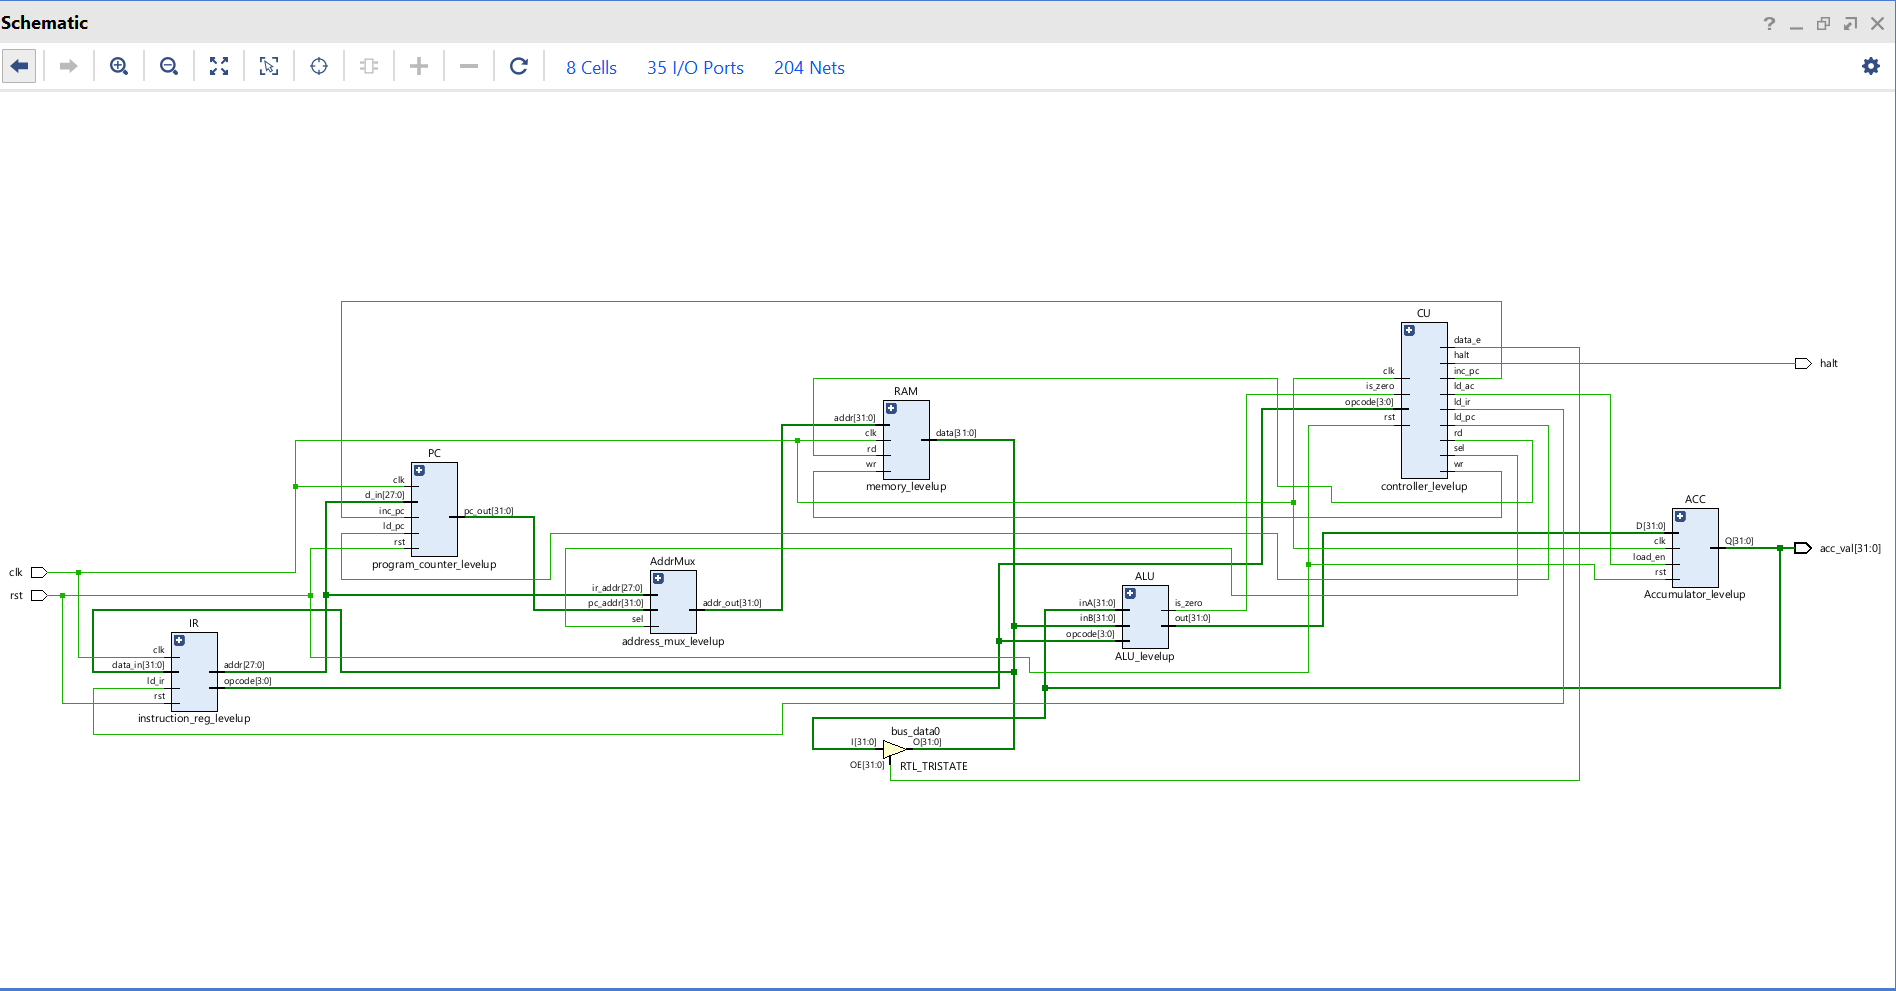
\includegraphics[width=1.0\textwidth]{sodo.png} 
    \caption{Sơ đồ mạch tích hợp hệ thống CPU nâng cao (RTL Schematic)}
    \label{fig:rtl_schematic_75}
\end{figure}

Sơ đồ RTL xác nhận toàn bộ 7 khối chức năng đã được kết nối chính xác theo kiến trúc thiết kế. Một số điểm kỹ thuật đáng lưu ý:
\begin{itemize}
    \item \textbf{Cơ chế Bus:} Khối \texttt{RTL\_TRISTATE} tại \texttt{bus\_data} đảm bảo dữ liệu từ Accumulator chỉ được đẩy lên bus khi tín hiệu $data\_e = 1$.
    \item \textbf{Mở rộng Opcode:} Đường tín hiệu \texttt{opcode[3:0]} (4-bit) kết nối trực tiếp giữa IR, ALU và Controller.
    \item \textbf{Tài nguyên:} Hệ thống sử dụng 8 Cells, 35 I/O Ports và 204 Nets, phản ánh quy mô của CPU 32-bit nâng cao.
\end{itemize}

\subsubsection{Mã kiểm thử hệ thống (Testbench)}
Đoạn mã Testbench dưới đây thực hiện nạp các giá trị vào RAM và thực thi chuỗi lệnh để kiểm tra các tính năng mới như \textbf{SUB} và \textbf{SHL}.

\begin{lstlisting}[caption={Mã Testbench cho CPU nâng cao}, label={lst:tb_75}]
`timescale 1ns / 1ps
module tb_CPU_levelup();
    reg clk; reg rst;
    wire halt; wire [31:0] acc_val;

    CPU_Top_levelup uut (
        .clk(clk), .rst(rst), .halt(halt), .acc_val(acc_val)
    );

    always #5 clk = ~clk;

    initial begin
        clk = 0; rst = 1;
        // Nap du lieu vao RAM
        uut.RAM.ram[10] = 32'd15;  
        uut.RAM.ram[11] = 32'd5;   
        uut.RAM.ram[12] = 32'd10;  

        // Nap chuong trinh
        uut.RAM.ram[0] = 32'h5000000A; // LDA 10 -> AC=15
        uut.RAM.ram[1] = 32'h2000000B; // ADD 11 -> AC=20
        uut.RAM.ram[2] = 32'h90000000; // SHL    -> AC=40
        uut.RAM.ram[3] = 32'h8000000C; // SUB 12 -> AC=30
        uut.RAM.ram[4] = 32'h6000000D; // STO 13
        uut.RAM.ram[5] = 32'h00000000; // HLT

        #15 rst = 0; 
        wait(halt == 1'b1);
        $finish;
    end
endmodule
\end{lstlisting}

\subsubsection{Giản đồ thời gian (Waveform)}
Quá trình tính toán được thể hiện chi tiết qua các chu kỳ xung nhịp trong giản đồ sóng:

\begin{figure}[H]
    \centering
    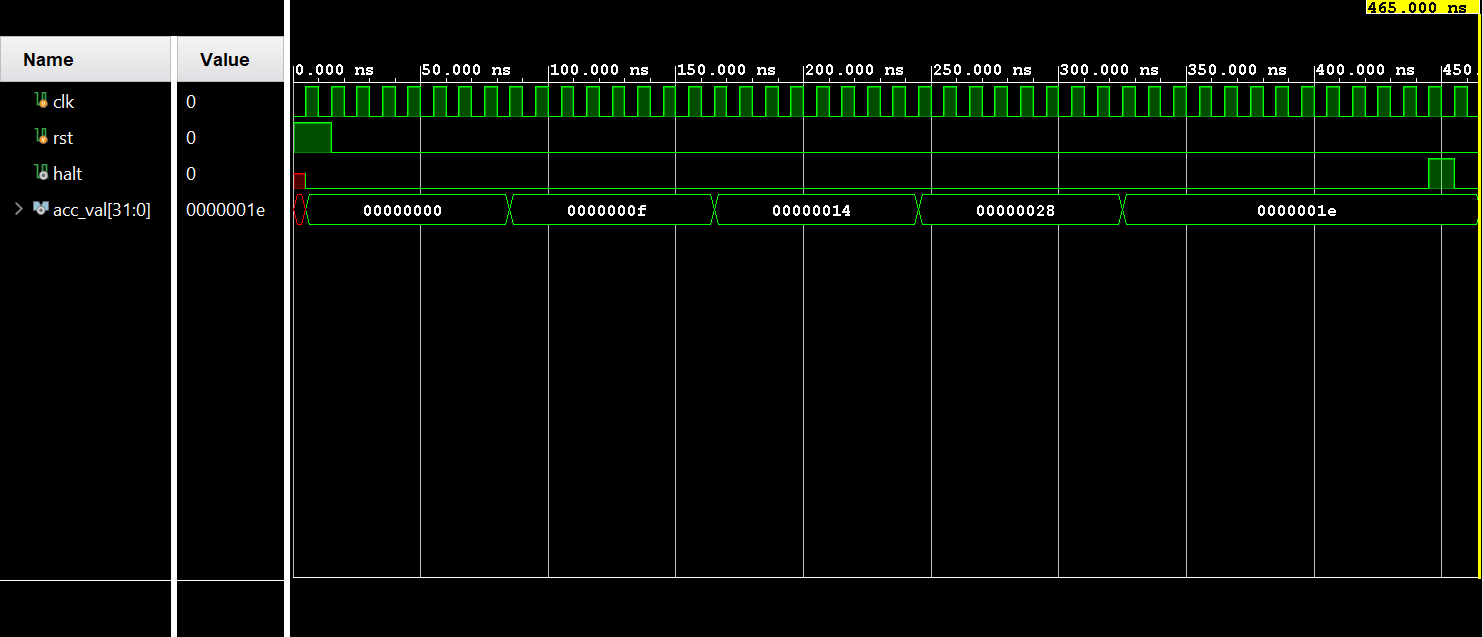
\includegraphics[width=1.0\textwidth]{wave.png} 
    \caption{Giản đồ thời gian mô phỏng CPU nâng cao}
    \label{fig:waveform_75}
\end{figure}

Logic toán học được thực thi qua các giai đoạn như sau:
\begin{enumerate}
    \item $ACC = RAM[10] = 15$
    \item $ACC = 15 + 5 = 20$
    \item $ACC = 20 \ll 1 = 40$ (Lệnh dịch trái SHL)
    \item $ACC = 40 - 10 = 30$ (Lệnh trừ SUB)
\end{enumerate}

\subsubsection{Kết quả xuất ra màn hình (Console Output)}
Kết quả kiểm thử cuối cùng được in ra cửa sổ Tcl Console xác nhận tính đúng đắn của toàn bộ hệ thống.

\begin{figure}[H]
    \centering
    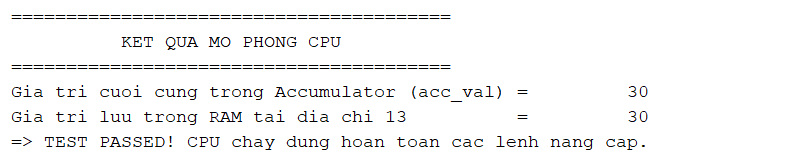
\includegraphics[width=0.8\textwidth]{console.png} 
    \caption{Kết quả Console mô phỏng hệ thống CPU nâng cao}
\end{figure}

\begin{quote}
    \textit{Giá trị cuối cùng trong Accumulator (\texttt{acc\_val}) = 30} \\
    \textit{Giá trị lưu trong RAM tại địa chỉ 13 = 30} \\
    \textbf{=> TEST PASSED! CPU chạy đúng hoàn toàn các lệnh nâng cấp.}
\end{quote}

Kết quả này khẳng định lệnh \textbf{STO} đã ghi thành công giá trị $30_{10}$ từ Accumulator vào địa chỉ 13 của bộ nhớ thông qua cơ chế bus dùng chung.



\subsection{Đánh giá hiệu năng hệ thống nâng cao}
Sau khi hoàn tất quá trình tổng hợp (Synthesis) trên Vivado, nhóm tiến hành thu thập và phân tích các thông số hiệu năng của phiên bản CPU nâng cao, bao gồm tài nguyên phần cứng, thời gian và năng lượng tiêu thụ.

\subsubsection{Phân tích tài nguyên sử dụng (Utilization Report)}

\begin{figure}[H]
    \centering
    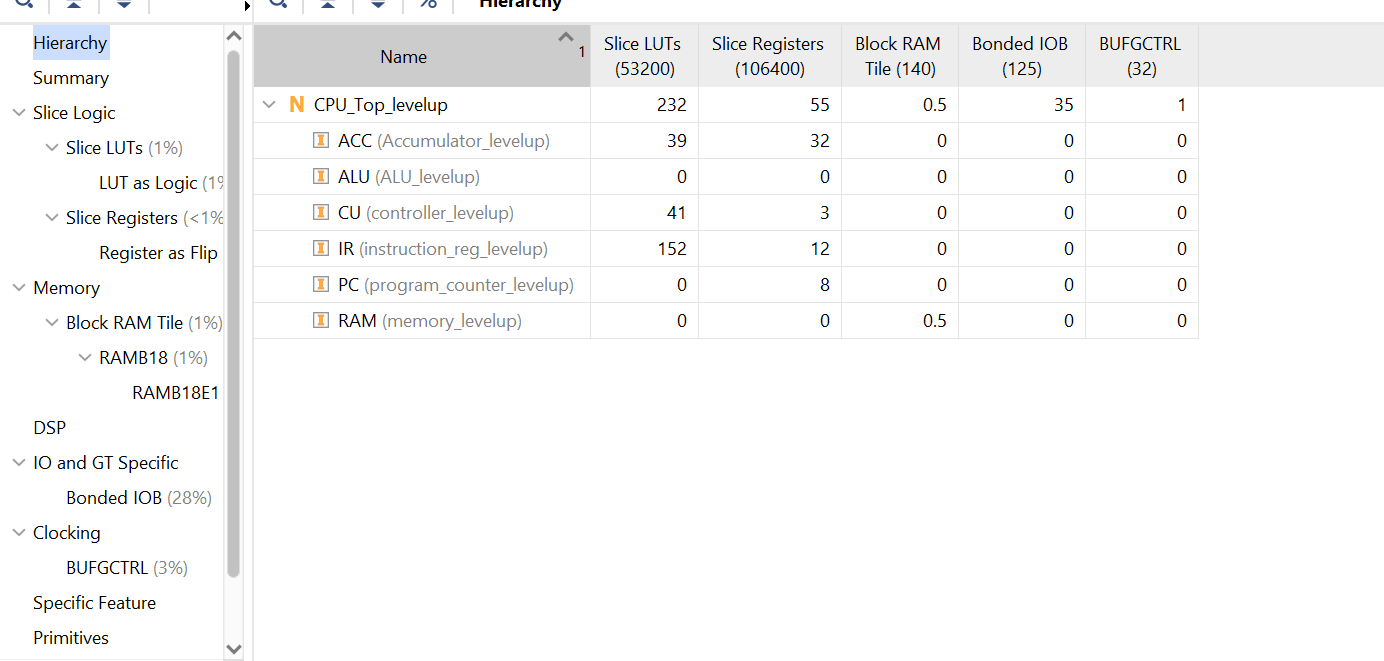
\includegraphics[width=1.0\textwidth]{til1.png} 
    \caption{Báo cáo tài nguyên Utilization chi tiết cho từng module (phiên bản nâng cao)}
    \label{fig:util_report}
\end{figure}

\begin{table}[H]
\centering
\footnotesize % Dùng mức nhỏ hơn small để an toàn tuyệt đối
\setlength{\tabcolsep}{3pt} % Thu hẹp khoảng cách giữa các cột
\begin{tabularx}{\textwidth}{|X|c|c|c|c|c|} % Cột đầu tiên tự co giãn
\hline
\textbf{Module} & \textbf{LUTs} & \textbf{Registers} 
& \textbf{BRAM} & \textbf{IOB} & \textbf{BUFG} \\
\hline
CPU\_Top\_levelup        & 232 & 55  & 0.5 & 35 & 1 \\
ACC (Accumulator)        & 39  & 32  & 0   & 0  & 0 \\
ALU (ALU\_levelup)       & 0   & 0   & 0   & 0  & 0 \\
CU (controller)          & 41  & 3   & 0   & 0  & 0 \\
IR (instruction)         & 152 & 12  & 0   & 0  & 0 \\
PC (prog\_counter)       & 0   & 8   & 0   & 0  & 0 \\
RAM (memory)             & 0   & 0   & 0.5 & 0  & 0 \\
\hline
\end{tabularx}
\caption{Báo cáo tài nguyên phiên bản CPU nâng cao}
\label{tab:util_levelup}
\end{table}

\textbf{Nhận xét:} \\
Hệ thống nâng cao tiêu thụ tổng cộng 232 LUTs và 55 Registers, tăng đáng kể so với phiên bản cơ bản (130 LUTs, 54 Registers). Sự gia tăng này chủ yếu đến từ các nguyên nhân sau:
\begin{itemize}
    \item \textbf{Khối IR:} Tăng mạnh nhất (từ 51 lên 152 LUTs) do phải xử lý opcode 4-bit và địa chỉ 28-bit. Việc mở rộng trường opcode khiến logic giải mã phức tạp hơn.
    \item \textbf{Khối CU:} Tăng nhẹ phản ánh việc bổ sung logic điều chỉnh cho 7 lệnh mới.
    \item \textbf{Khối ALU:} Tiêu thụ 0 LUTs do Vivado tối ưu hóa thành các primitives có sẵn.
    \item \textbf{Khối RAM:} Ánh xạ vào 0.5 Block RAM Tile, giữ nguyên so với phiên bản cơ bản.
\end{itemize}

Bảng dưới đây so sánh tài nguyên giữa hai phiên bản:

\begin{table}[H]
\centering
\begin{tabular}{|l|c|c|c|}
\hline
\textbf{Tiêu chí} & \textbf{Phiên bản cơ bản} & \textbf{Phiên bản nâng cao} & \textbf{Tăng} \\
\hline
Slice LUTs      & 130  & 232  & +78\% \\
Slice Registers & 54   & 55   & +2\%  \\
Block RAM Tile  & 0.5  & 0.5  & 0\%   \\
Bonded IOB      & 3    & 35   & +1067\% \\
\hline
\end{tabular}
\caption{So sánh tài nguyên phiên bản cơ bản và nâng cao}
\label{tab:util_compare}
\end{table}

Sự tăng vọt của \textbf{Bonded IOB} (từ 3 lên 35) phát sinh từ việc bổ sung ngõ ra \texttt{acc\_val[31:0]} (32 chân) để hiển thị kết quả ra LED trên FPGA.

\subsubsection{Phân tích thời gian (Timing Analysis)}

\begin{figure}[H]
    \centering
    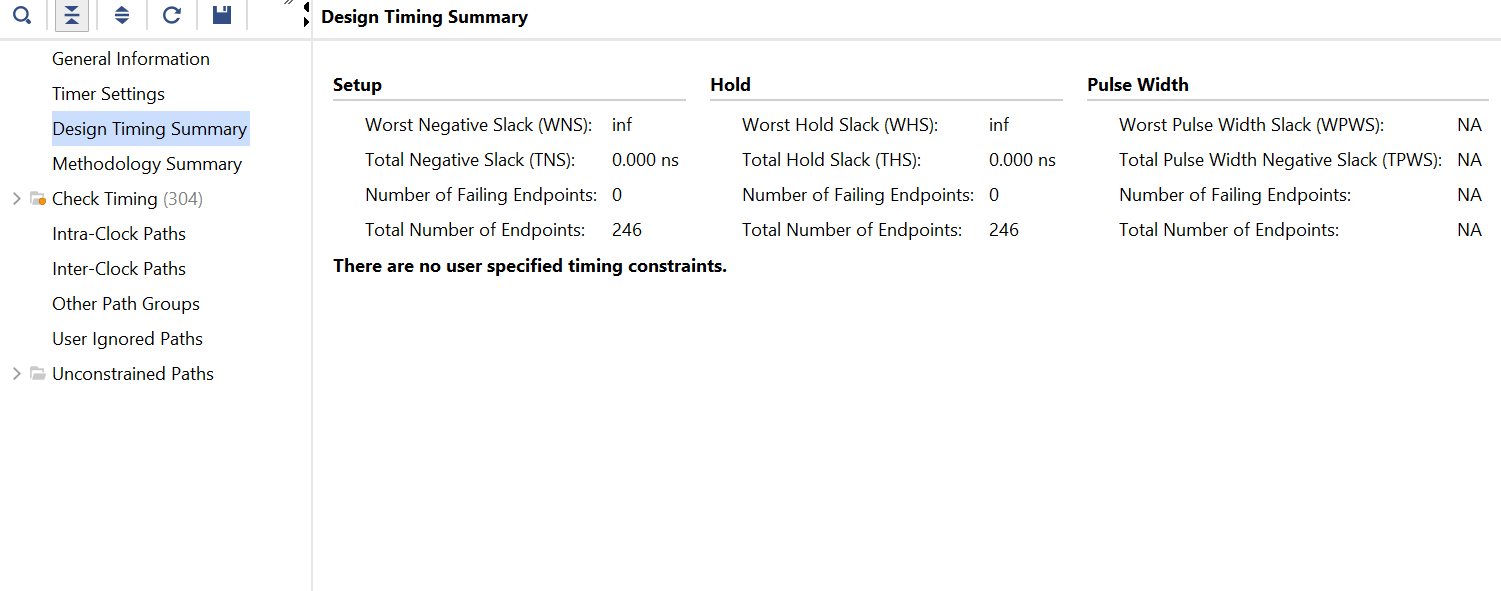
\includegraphics[width=1.0\textwidth]{timing.png} 
    \caption{Báo cáo phân tích thời gian Timing Summary (phiên bản nâng cao)}
    \label{fig:timing_report}
\end{figure}

\textbf{Nhận xét:}
\begin{itemize}
    \item Chỉ số \textbf{TNS (Total Negative Slack)} bằng 0.000 ns, khẳng định thiết kế không vi phạm ràng buộc thời gian hoặc lỗi chạy đua tín hiệu.
    \item Tổng số Endpoints tăng từ 211 lên 246 do bổ sung tập lệnh mới.
    \item Hệ thống hoàn toàn đáp ứng các ứng dụng yêu cầu tần số hoạt động tiêu chuẩn trên chip Artix-7.
\end{itemize}

\subsubsection{Phân tích năng lượng tiêu thụ (Power Analysis)}

\begin{figure}[H]
    \centering
    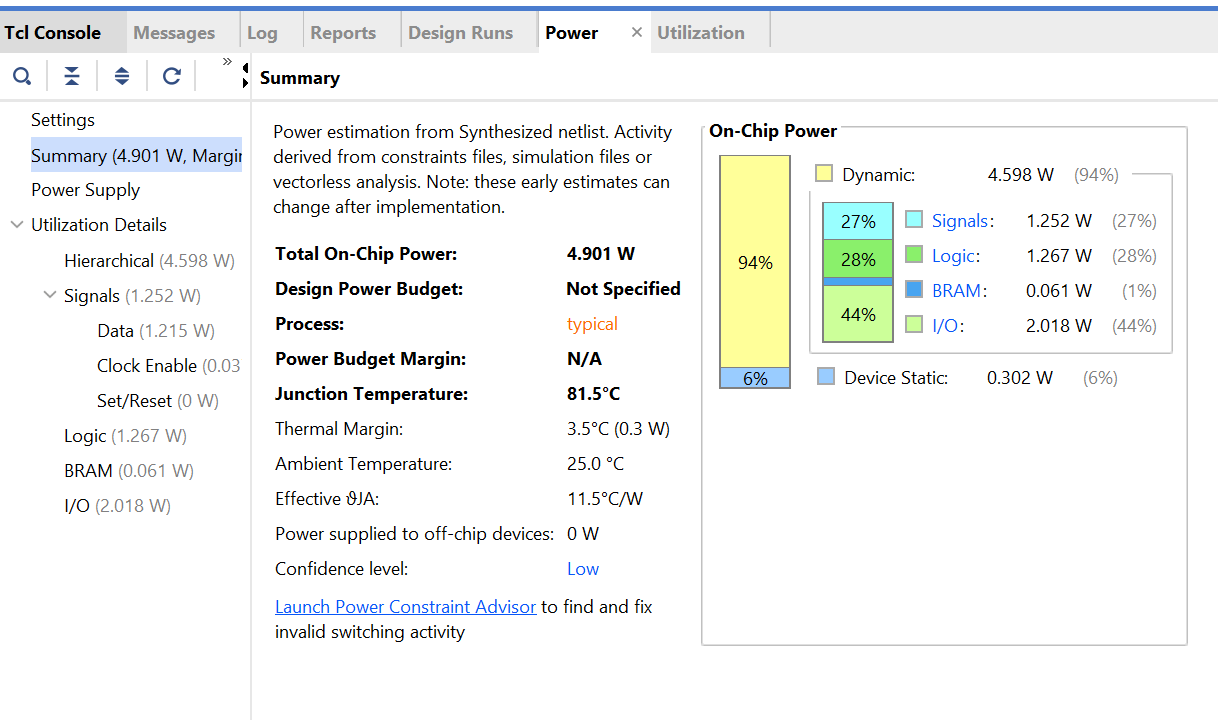
\includegraphics[width=0.9\textwidth]{pow.png} 
    \caption{Báo cáo ước tính năng lượng tiêu thụ (phiên bản nâng cao)}
    \label{fig:power_report}
\end{figure}

\textbf{Nhận xét:}
\begin{itemize}
    \item \textbf{Tổng công suất:} Đạt 4.901 W (tăng so với 1.952 W ở bản cơ bản). Nguyên nhân chính là do I/O chiếm tới 44\% (do 32 chân \texttt{acc\_val}).
    \item \textbf{Nhiệt độ Junction:} Đạt 81.5°C, vẫn nằm trong giới hạn an toàn ($< 85$°C) nhưng cần lưu ý về tản nhiệt khi triển khai thực tế.
\end{itemize}

Bảng dưới đây tổng hợp so sánh hiệu năng giữa hai phiên bản:

\begin{table}[H]
\centering
\small
\begin{tabular}{|l|c|c|}
\hline
\textbf{Thông số} & \textbf{Phiên bản cơ bản} & \textbf{Phiên bản nâng cao} \\
\hline
Tổng công suất       & 1.952 W  & 4.901 W  \\
Công suất động       & 93\%     & 94\%     \\
Công suất I/O        & 0.194 W  & 2.018 W  \\
Nhiệt độ Junction    & 47.5°C   & 81.5°C   \\
Thermal Margin       & 3.1°C    & 3.5°C (0.3 W) \\
TNS                  & 0.000 ns & 0.000 ns \\
Failing Endpoints    & 0        & 0        \\
Tổng Endpoints       & 211      & 246      \\
\hline
\end{tabular}
\caption{So sánh hiệu năng tổng thể giữa hai phiên bản CPU}
\label{tab:perf_compare}
\end{table}


    \newpage
  \section*{Phụ lục: Mã nguồn chương trình}
    \addcontentsline{toc}{section}{Phụ lục: Mã nguồn chương trình}
    
    Toàn bộ mã nguồn Verilog, các file Testbench và báo cáo của dự án thiết kế CPU RISC được lưu trữ tại hệ thống quản lý phiên bản GitHub theo đường dẫn dưới đây:
    
    \begin{itemize}
        \item \textbf{Repository URL:} \url{https://github.com/thanh-tran-tien206/RISC-CPU-BTL-HDL.git}
    \end{itemize}

\end{document}